% Created 2016-08-31 Wed 19:13
\documentclass[9pt]{beamer}
\usepackage[utf8]{inputenc}
\usepackage[T1]{fontenc}
\usepackage{fixltx2e}
\usepackage{graphicx}
\usepackage{longtable}
\usepackage{float}
\usepackage{wrapfig}
\usepackage{soul}
\usepackage{textcomp}
\usepackage{marvosym}
\usepackage{wasysym}
\usepackage{latexsym}
\usepackage{amssymb}
\usepackage{hyperref}
\tolerance=1000
\mode<beamer>{\usetheme{Warsaw}}
\mode<beamer>{\setbeamertemplate{blocks}[rounded][shadow=false]}
\mode<beamer>{\addtobeamertemplate{block begin}{\pgfsetfillopacity{0.8}}{\pgfsetfillopacity{1}}}
\mode<beamer>{\setbeamercolor{structure}{fg=orange}}
\mode<beamer>{\setbeamercovered{transparent}}
\AtBeginSection[]{\begin{frame}<beamer>\frametitle{Topic}\tableofcontents[currentsection]\end{frame}}
\usepackage{subcaption}
\usepackage{multimedia}
\usepackage{tikz}
\usepackage{subfigure,subfigmat}
\usepackage{threeparttable}
\usetikzlibrary{shapes,arrows,shadows}
\usepackage{bm, amssymb, amsmath, array, pdfpages}
\newcommand{\bv}[1]{\mathbf{#1}}
\newcommand{\diff}[2]{\frac{\partial #1}{\partial #2}}
\newcommand{\beq}[0]{\begin{equation}}
\newcommand{\eeq}[0]{\end{equation}}
\newcommand{\beqa}[0]{\begin{eqnarray}}
\newcommand{\eeqa}[0]{\end{eqnarray}}
\newcommand{\beqq}[0]{\begin{equation*}}
\newcommand{\eeqq}[0]{\end{equation*}}
\newcommand{\bs}[1]{\boldsymbol{#1}}
\newcommand{\ip}[2]{\langle #1, #2\rangle}
\providecommand{\alert}[1]{\textbf{#1}}

\title{Modeling and Uncertainty Quantification for Airfoil Icing}
\author{Anthony DeGennaro \newline Clarence W. Rowley III \newline Luigi Martinelli \newline Princeton University}
\date{Final Public Oral \\ Princeton, NJ \\ September 2016}
\hypersetup{
  pdfkeywords={},
  pdfsubject={},
  pdfcreator={Emacs Org-mode version 7.9.3f}}

\begin{document}

\maketitle

\begin{frame}
\frametitle{Outline}
\setcounter{tocdepth}{3}
\tableofcontents
\end{frame}



% Define my settings

\graphicspath{{Figures/}}
% Add Princeton shield logo
\addtobeamertemplate{frametitle}{}{%
\begin{tikzpicture}[remember picture,overlay]
\node[anchor=north east,yshift=2pt] at (current page.north east) {
\includegraphics[height=0.7cm]{Shield}};
\end{tikzpicture}}
%


\institute{Princeton University}

\section{Motivation/Background}
\label{sec-1}
\begin{frame}
\frametitle{Introduction}
\label{sec-1-1}

\textbf{What is aircraft icing?}
\begin{itemize}
\item In-flight accumulation of ice on aircraft structure
\begin{itemize}
\item Aircraft nacelle
\item Engine (cowling, inlet, compressor blades)
\item Lifting surfaces (wings and stabilizers)
\item Flight instruments (pitot tube)
\end{itemize}
\end{itemize}

\vspace*{-0.0cm}\begin{figure}
      \subfigure[Nacelle icing]{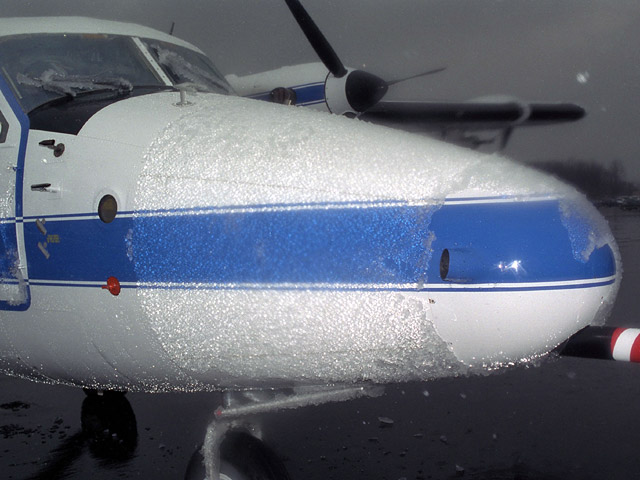
\includegraphics[width=0.3\textwidth]{NacelleIcing.jpg}}
      \subfigure[Wing icing]{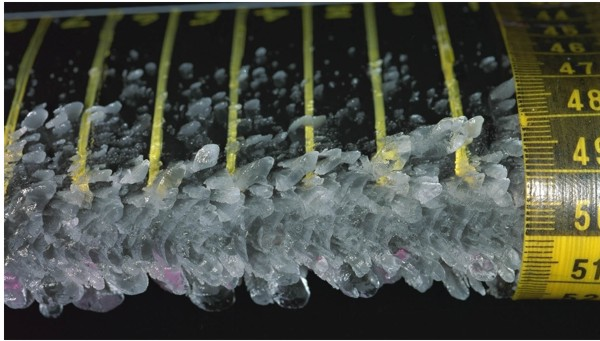
\includegraphics[width=0.3\textwidth]{WingIcingIntro}}
      \subfigure[Engine icing]{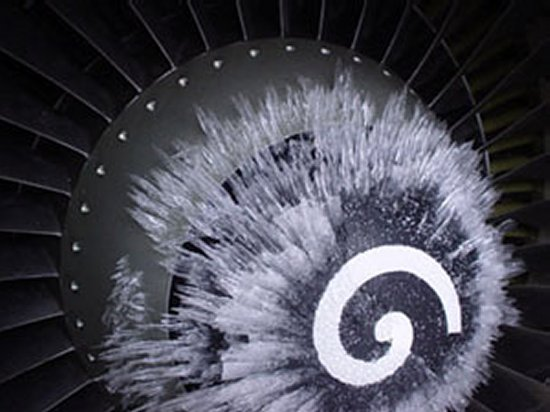
\includegraphics[width=0.3\textwidth]{EngineIcingIntro}}
      \caption{Examples of structural aircraft icing.}
\end{figure}
\end{frame}
\begin{frame}
\frametitle{Introduction}
\label{sec-1-2}

\textbf{Why is aircraft icing dangerous?}
\begin{itemize}
\item Nacelle icing
\begin{itemize}
\item Increase profile drag
\end{itemize}
\item Engine icing
\begin{itemize}
\item Disrupt airflow into engine
\item Cause compressor blade stall
\item Damage to engine blades
\end{itemize}
\item Instrument icing
\begin{itemize}
\item Causes incorrect Pitot tube speed/pressure measurements
\end{itemize}
\item Wing/stabilizer icing
\begin{itemize}
\item Decreases lift, increases drag
\item Causes unpredictable stall characteristics
\item Causes loss of control surface effectiveness
\end{itemize}
\end{itemize}
\emph{We limit our focus to wing icing in what follows}
\end{frame}
\begin{frame}
\frametitle{Introduction}
\label{sec-1-3}

\textbf{How does wing ice form?}
\begin{itemize}
\item Warm, humid air is convected upward to cooler, higher altitudes
\item Liquid water droplets condense out of supersaturated air
\item Atmospheric droplets can remain in \emph{supercooled} liquid state
\begin{itemize}
\item Sparsity of nucleation sites for heterogeneous crystallization
\item Homogeneous crystallization does not begin until extreme cold ($\approx -48^\circ C$)
\end{itemize}
\item Airplanes provide great nucleation sites for ice crystallization
\end{itemize}
\vspace*{-0.0cm}\begin{figure}
      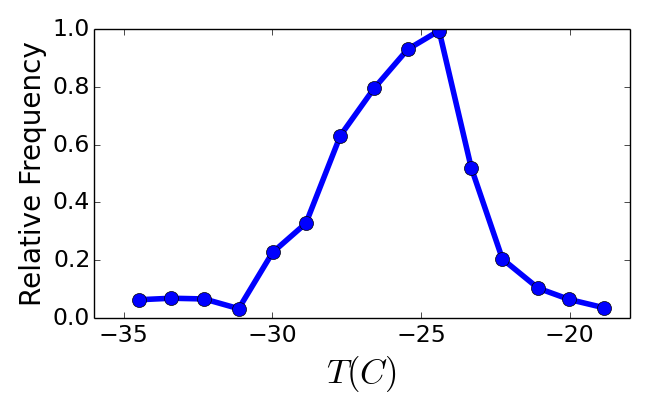
\includegraphics[width=0.4\textwidth]{DropletFreezingIntro.png}
      \caption{Freezing temperature distribution (droplet diameter =
      35 $\mu m$)\footnote{\tiny Dorsch and
      Hacker. \emph{Photomicrographic investigation of spontaneous
      freezing temperatures of supercooled water droplets.} NACA-TN
      2142, 1950.}  } \end{figure}
\end{frame}
\begin{frame}
\frametitle{Introduction}
\label{sec-1-4}

\textbf{How does wing ice form?}
\begin{itemize}
\item Details of ice formation controlled by heat transfer mechanisms
\begin{itemize}
\item Aerodynamic convective cooling
\item Evaporation/sublimation
\end{itemize}
\item \emph{Rime ice:} cold, dry conditions --> droplets freeze immediately upon impact
\item \emph{Glaze ice:} warm, wet conditions --> partial freezing plus ``runback'' water
\end{itemize}

\vspace*{-0.5cm}\begin{figure} \subfigure[Rime
      Ice]{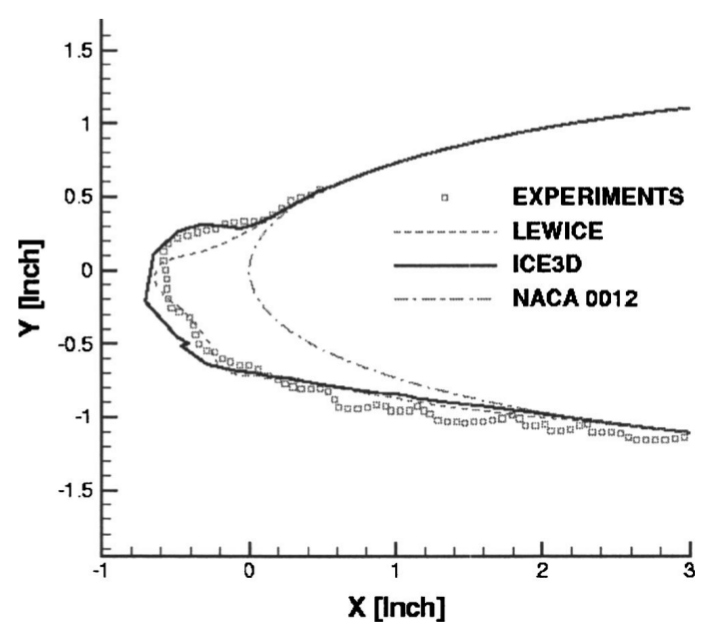
\includegraphics[width=0.3\textwidth]{Habashi2006Rime.png}}
      \subfigure[Horn
      Ice]{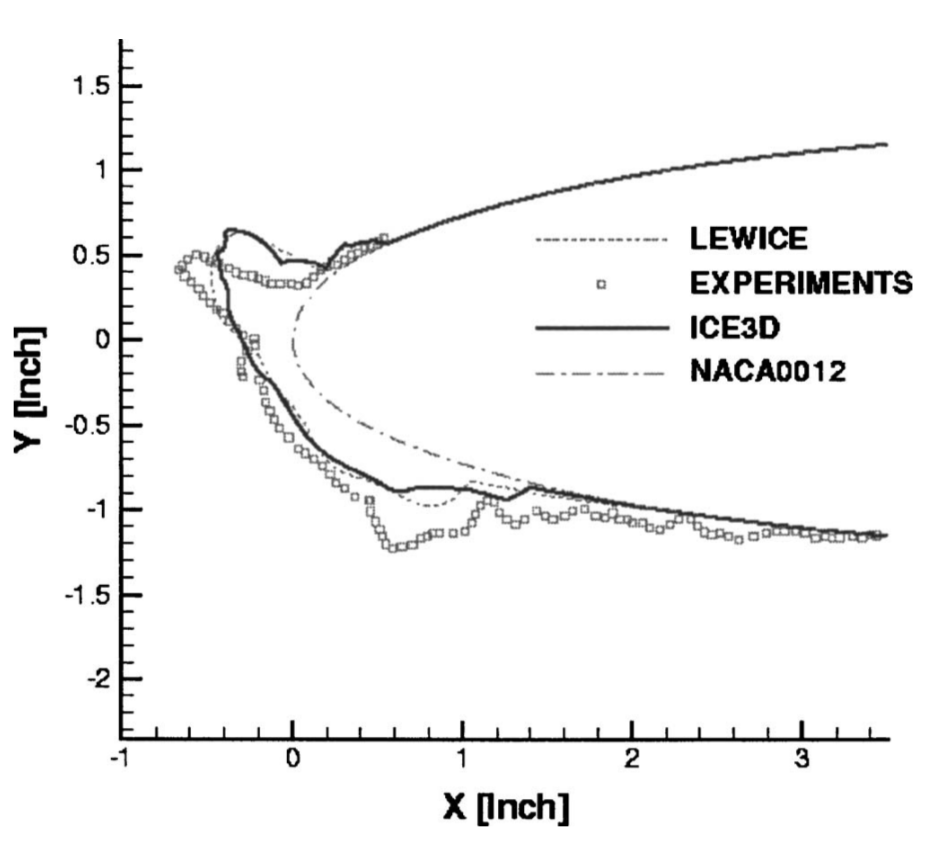
\includegraphics[width=0.3\textwidth]{Habashi2006Horn.png}}
      \caption{Canonical examples of rime/horn ice\footnote{\tiny Beaugendre
      et. al. \emph{Development of a Second Generation In-Flight
      Simulation Code}. J. Fluids Engineering, 2006.}}  \end{figure}
\end{frame}
\begin{frame}
\frametitle{Introduction}
\label{sec-1-5}

\textbf{Wing icing deteriorates airfoil aerodynamics}
\begin{itemize}
\item Leading edge flow separation bubble
\item Lower lift, higher drag
\item Unpredictable stall
\end{itemize}

\vspace*{-0.0cm}\begin{figure}
    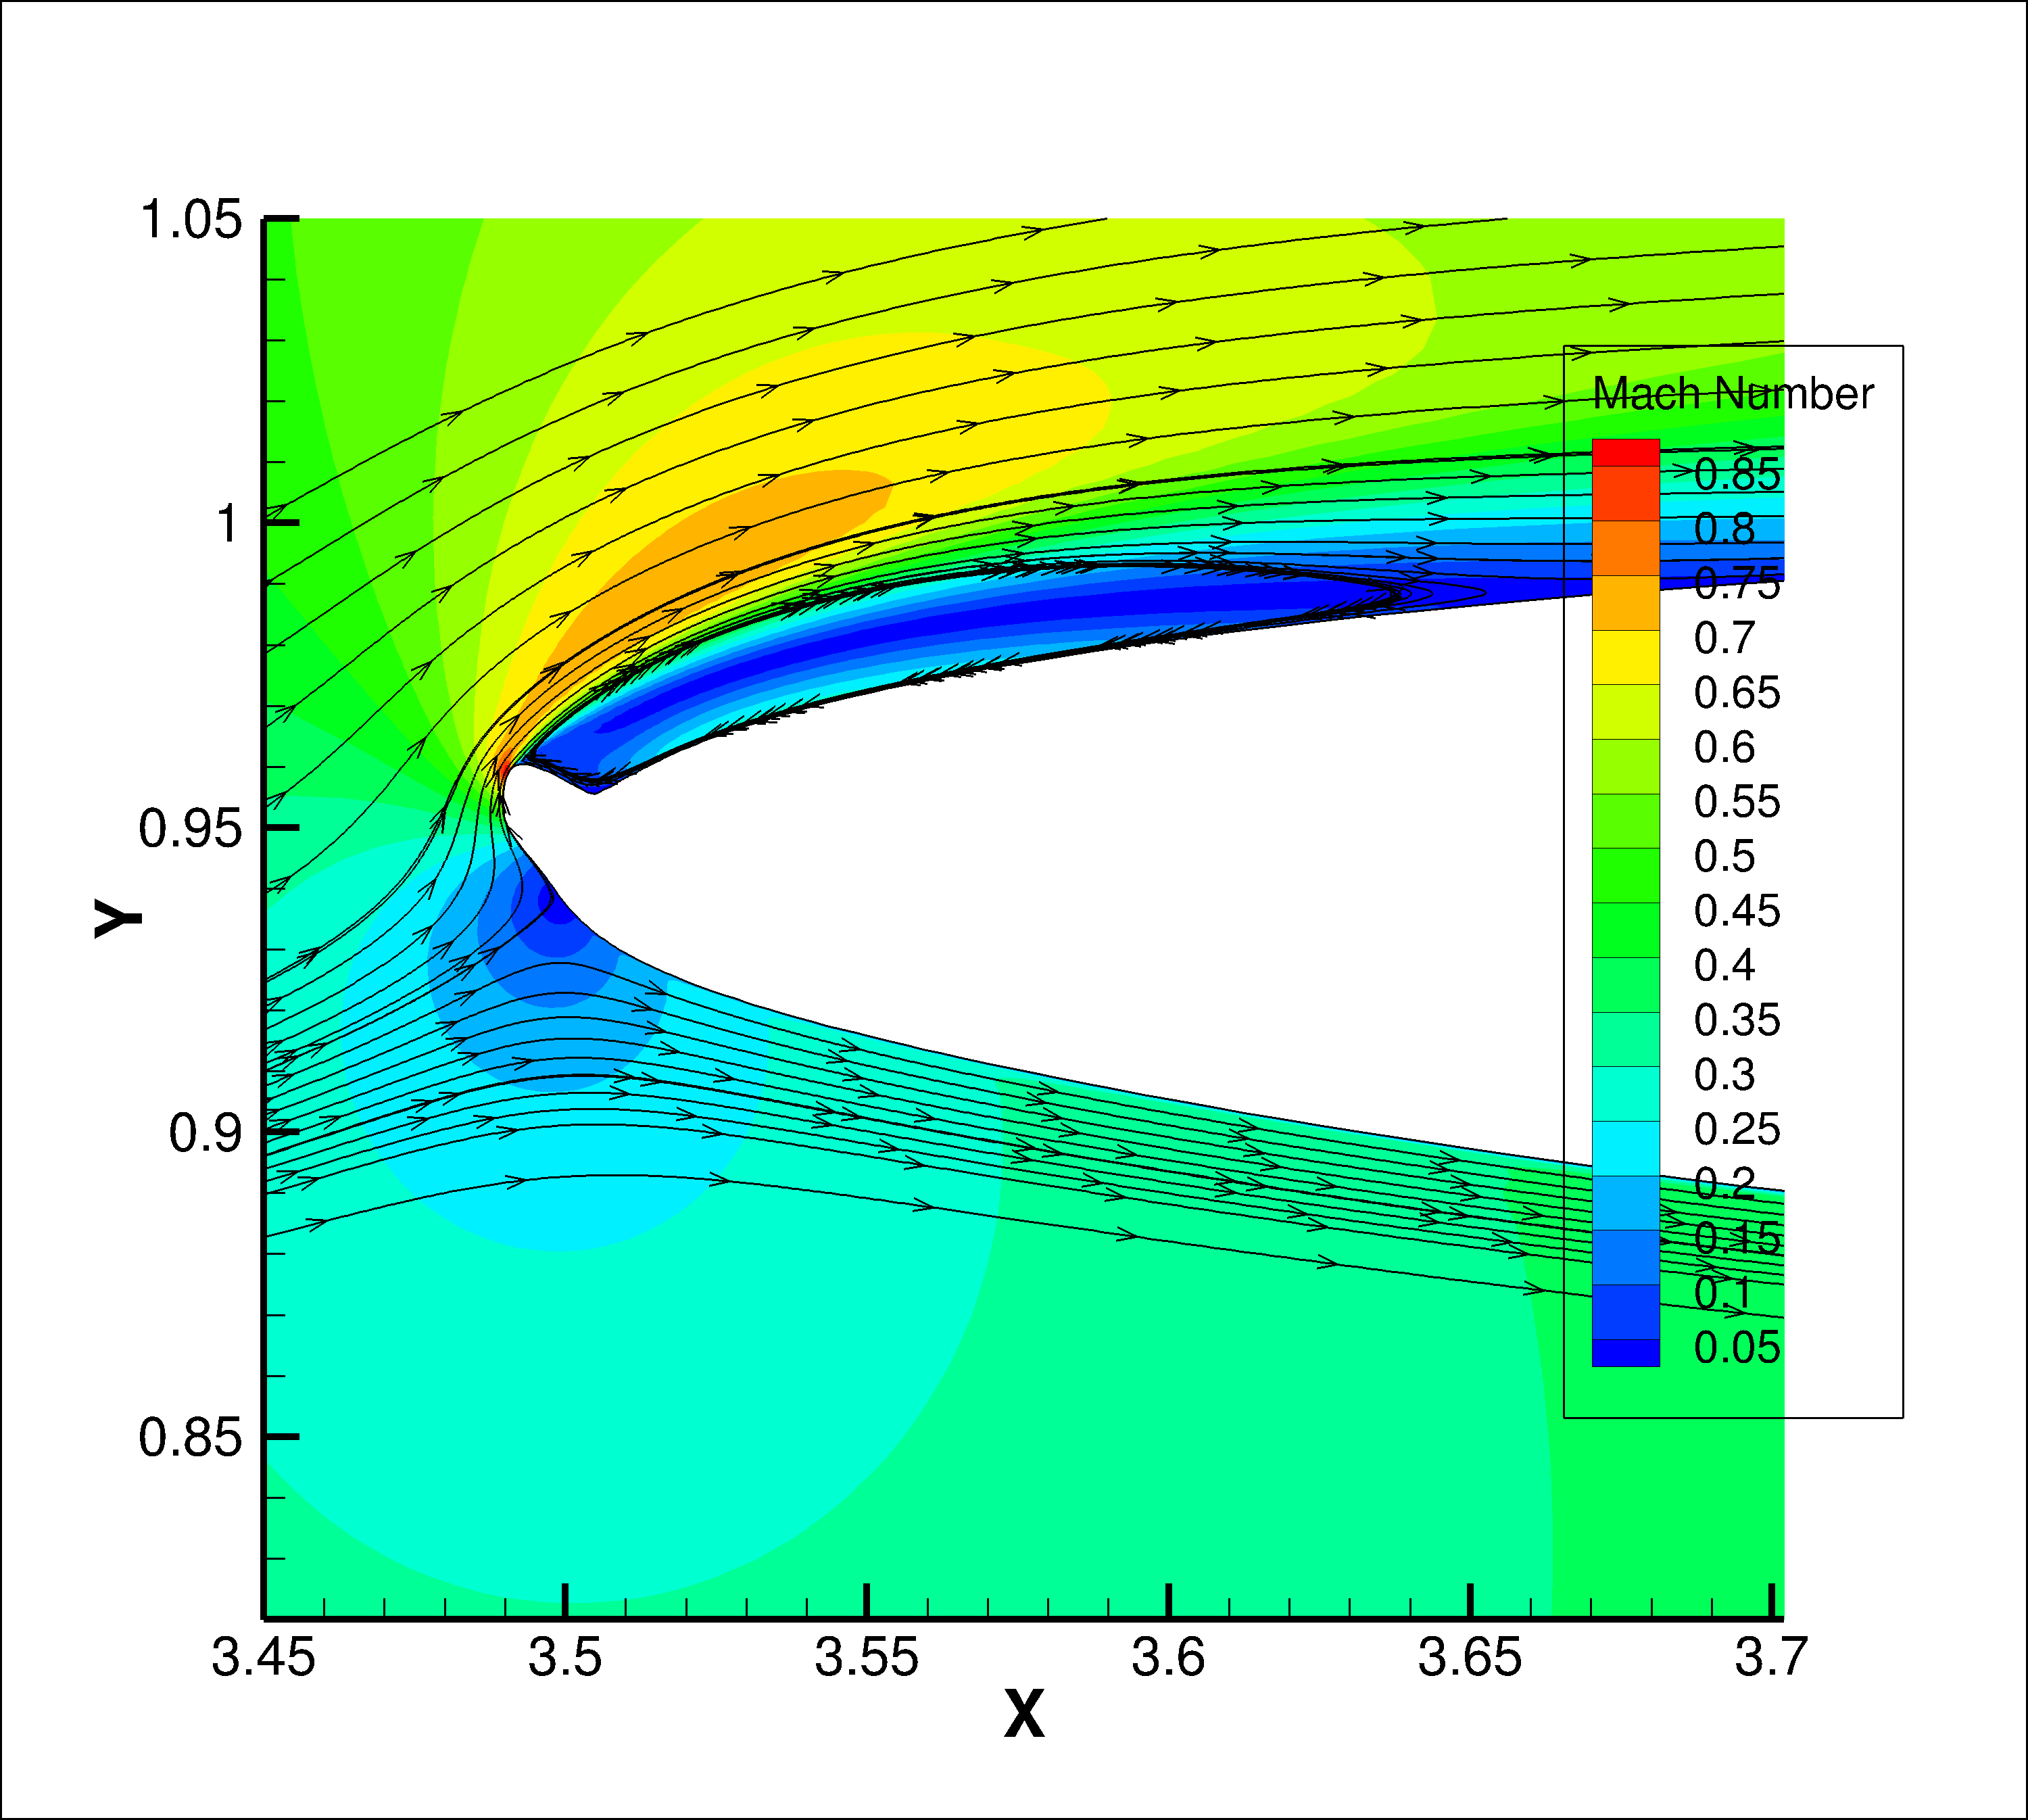
\includegraphics[width=0.4\textwidth]{BadHorn.png}
    \caption{Leading edge horn separation}
\end{figure}
\end{frame}
\begin{frame}
\frametitle{Introduction}
\label{sec-1-6}

\textbf{Significant ice shape variation, sensitivity to physical parameters}\footnote{Addy, H.E. \emph{Ice Accretions and Icing Effects for Modern Airfoils}. NASA TR 2000-210031.
 }
\begin{itemize}
\item Complex physics (aero-thermodynamics, macro/micro scale physics)
\item Uncertainty in physical parameters
\end{itemize}

\vspace*{-0.0cm}\begin{figure}
      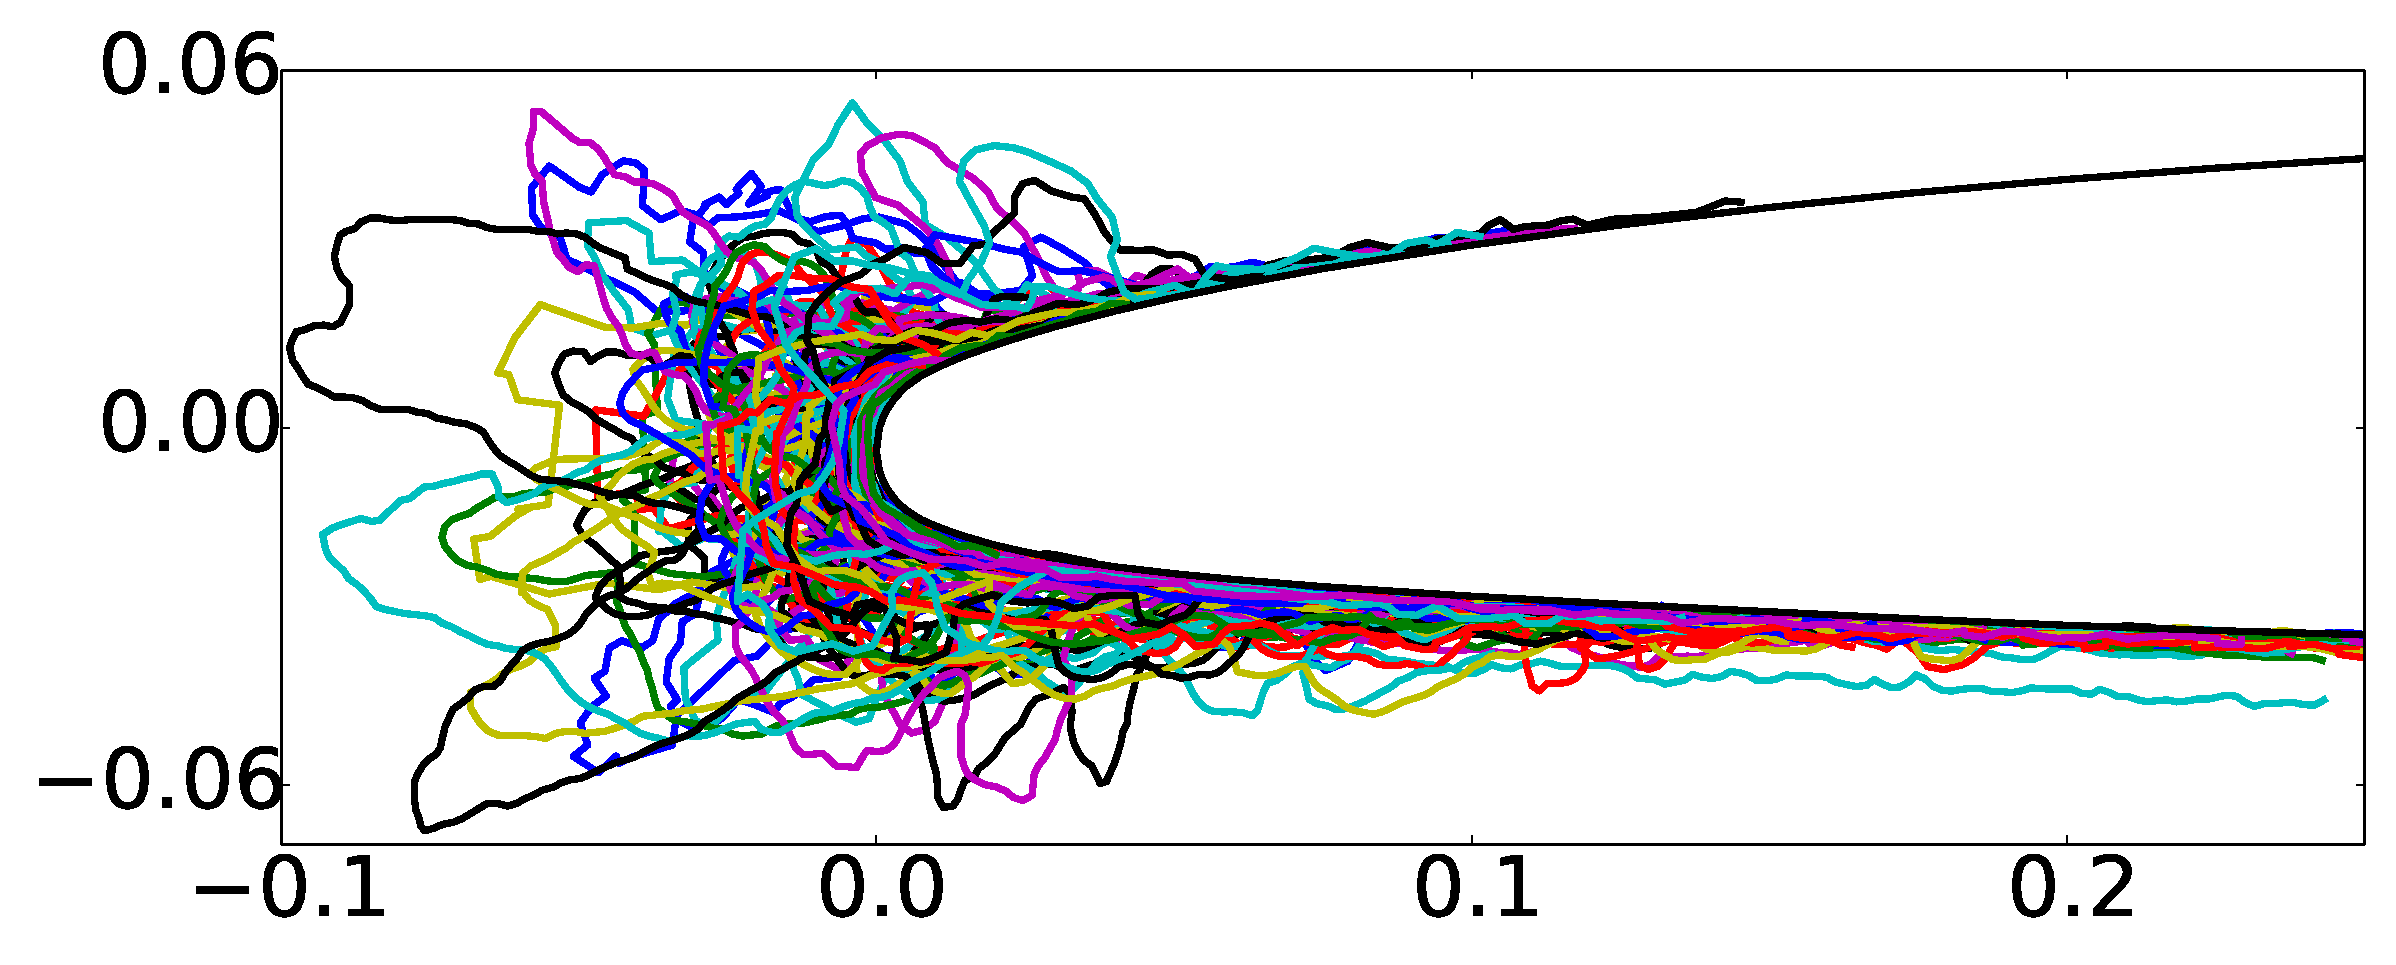
\includegraphics[width=0.75\textwidth]{GlobalDataSet}
      \caption{Wind tunnel experimental ice shapes}
\end{figure}
\end{frame}
\begin{frame}
\frametitle{Introduction}
\label{sec-1-7}

\textbf{Different types of ice accretion}\footnote{Beaugendre et. al. \emph{Development of a Second Generation In-Flight Simulation Code}. J. Fluids Engineering, 2006.
 }
\begin{itemize}
\item ``Horns'', ``ridges'', ``lobster tails'' refer to shape
\item ``Glaze'', ``rime'' refer to icing thermodynamics
\end{itemize}

\vspace*{-0.0cm}\begin{figure}
      \subfigure[Rime Ice]{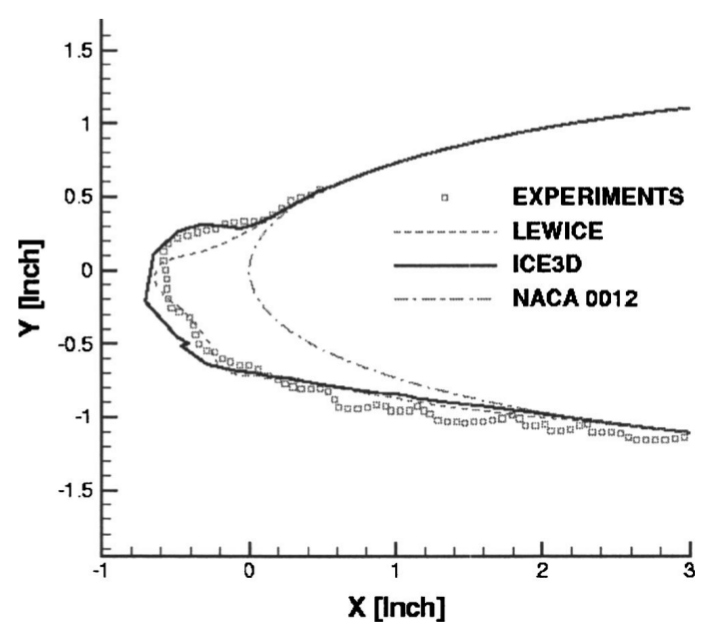
\includegraphics[width=0.4\textwidth]{Habashi2006Rime.png}}
      \subfigure[Horn Ice]{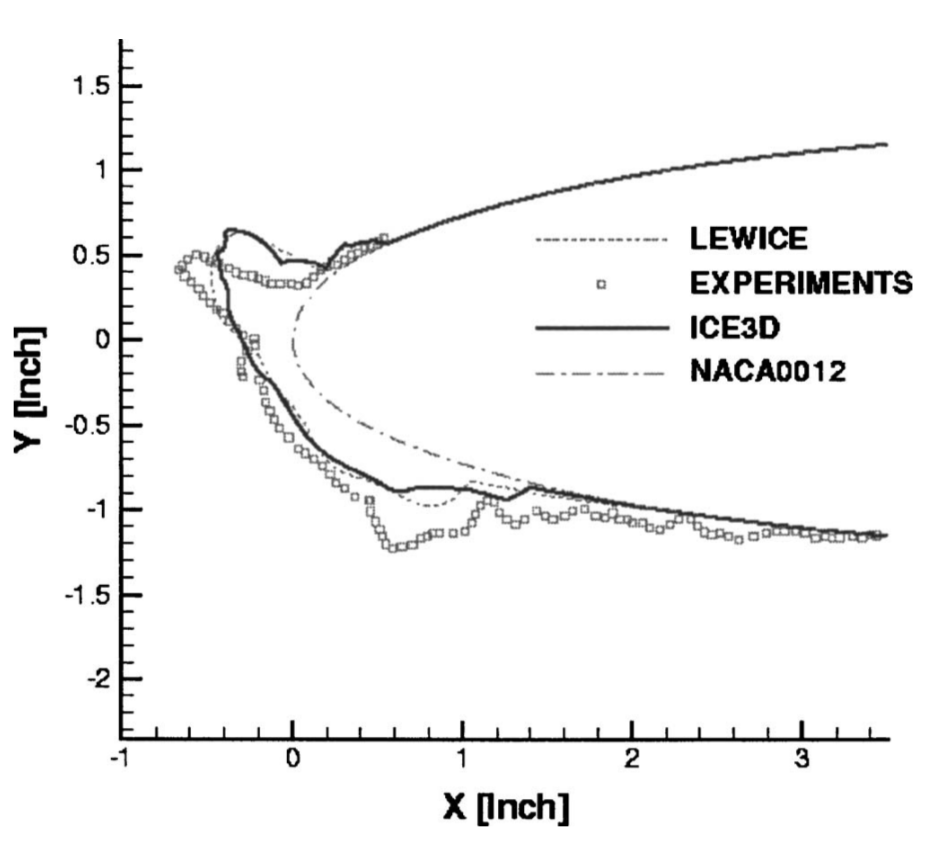
\includegraphics[width=0.4\textwidth]{Habashi2006Horn.png}}
 
\end{figure}
\end{frame}
\begin{frame}
\frametitle{Introduction}
\label{sec-1-8}

\textbf{Research Goals}
\begin{itemize}
\item Apply uncertainty quantification techniques to explore statistical
  efffects of uncertain icing parameters on ice shape and aerodynamics
\begin{itemize}
\item Polynomial chaos expansions (PCE)
\item Tensor/sparse grid collocation sampling
\item 2D steady-state RANS solver for aerodynamic assessment
\end{itemize}
\item Build ice shape model from data
\begin{itemize}
\item Aggregate ice shape database
\item Cluster shapes using spectral graph partitioning
\item Model shape variation using Proper Orthogonal Decomposition (POD)
\end{itemize}
\item Quantify effects of physical uncertainties in aero-thermodynamics
\begin{itemize}
\item Build a computational ice-accretion code
\item UQ on governing parameters (LWC, temperature, accretion time, etc.)
\end{itemize}
\end{itemize}
\end{frame}
\begin{frame}
\frametitle{Introduction}
\label{sec-1-9}

\textbf{Thesis Structure}
\begin{itemize}
\item Heuristic UQ
\begin{itemize}
\item Ice shape scaling parameters
\item Verify PCE techniques against Monte Carlo simulations
\end{itemize}
\item Data-based UQ
\begin{itemize}
\item Build ice shape model from data
\item Clustering + POD
\end{itemize}
\item Computational UQ
\begin{itemize}
\item Build computational ice accretion code
\item Droplet impingement + thermodynamic PDE solvers
\end{itemize}
\end{itemize}
\end{frame}
\section{Heuristic UQ}
\label{sec-2}
\begin{frame}
\frametitle{Canonical Ice Shapes}
\label{sec-2-1}

\begin{itemize}
\item \textbf{Basic ice shapes}\footnote{Papadakis et. al. \emph{Aerodynamic Scaling Experiments with Simulated Ice Accretions}. AIAA 2001-0833.
 }
\end{itemize}
\centering
\vspace{-0.5cm}
\begin{minipage}[t]{0.4\linewidth}
\begin{figure}[t]
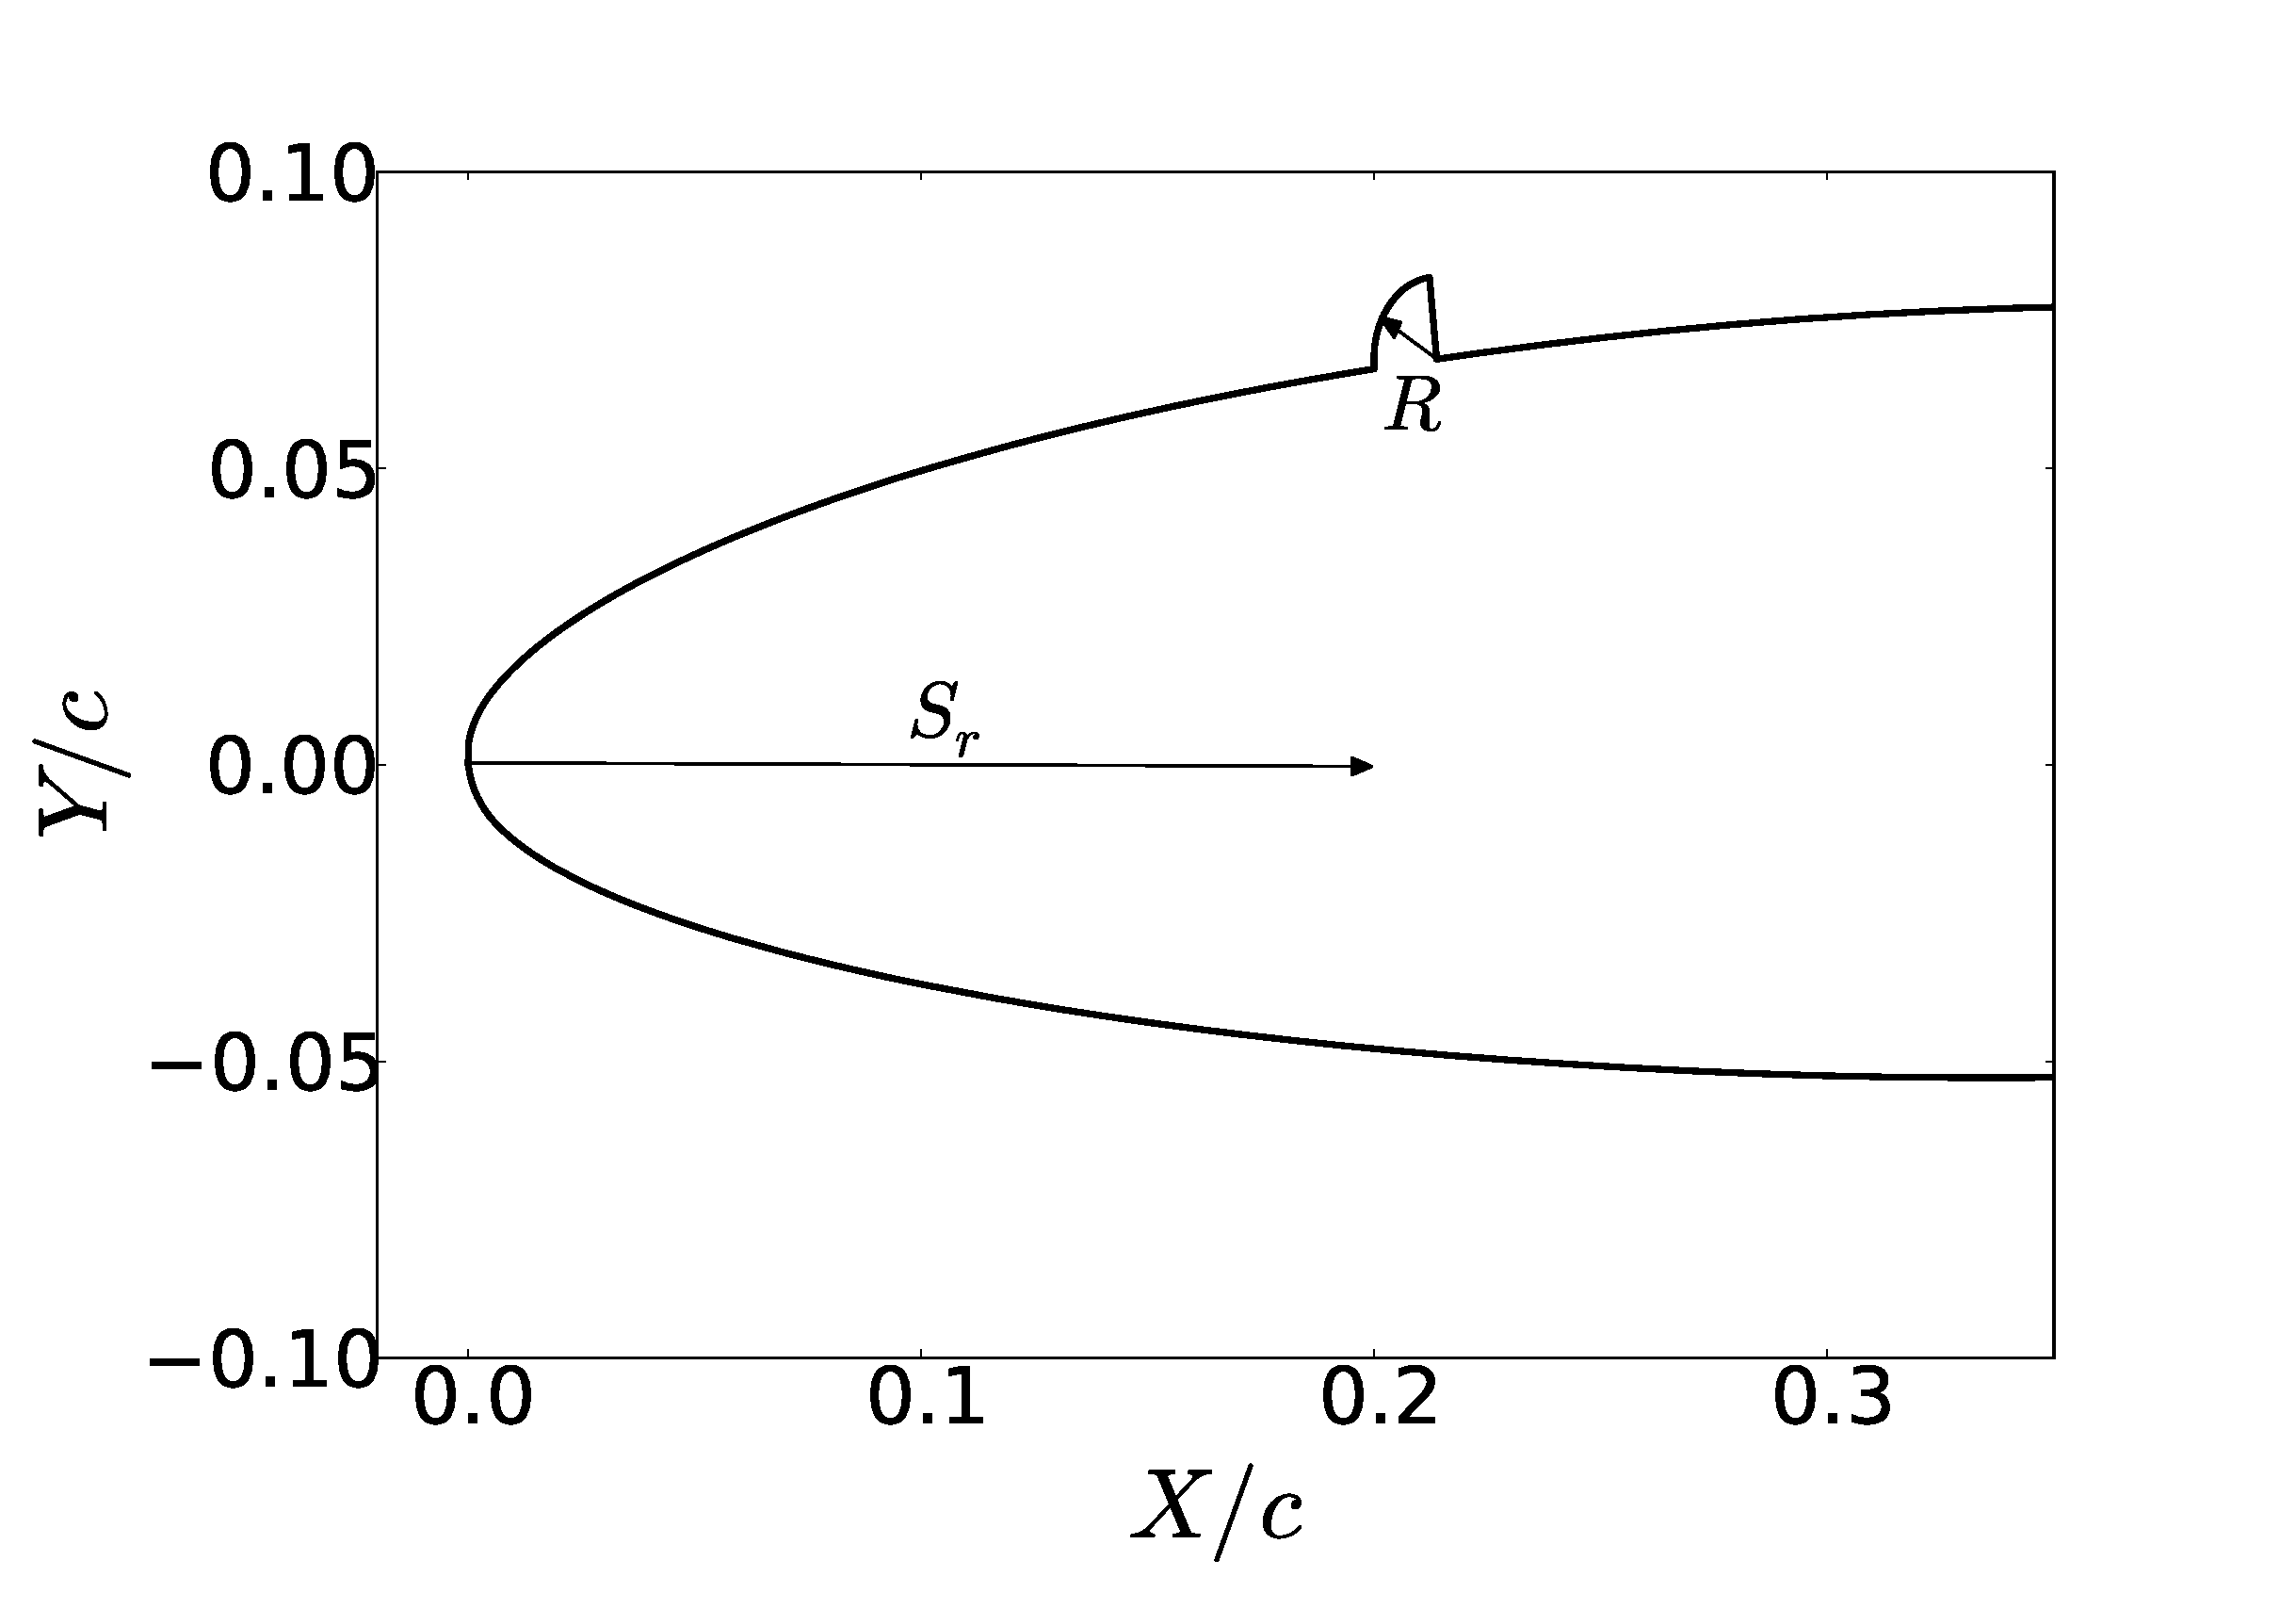
\includegraphics[width=0.95\textwidth]{RidgeParameters}
\caption{Ridge Ice}
\end{figure}
\vspace{-0.5cm}
\begin{itemize}
\item Forms aft of deicing mechanism
\item Runback water refreezes to form step
\end{itemize}
\end{minipage}
\begin{minipage}[t]{0.4\linewidth}
\begin{figure}[t]
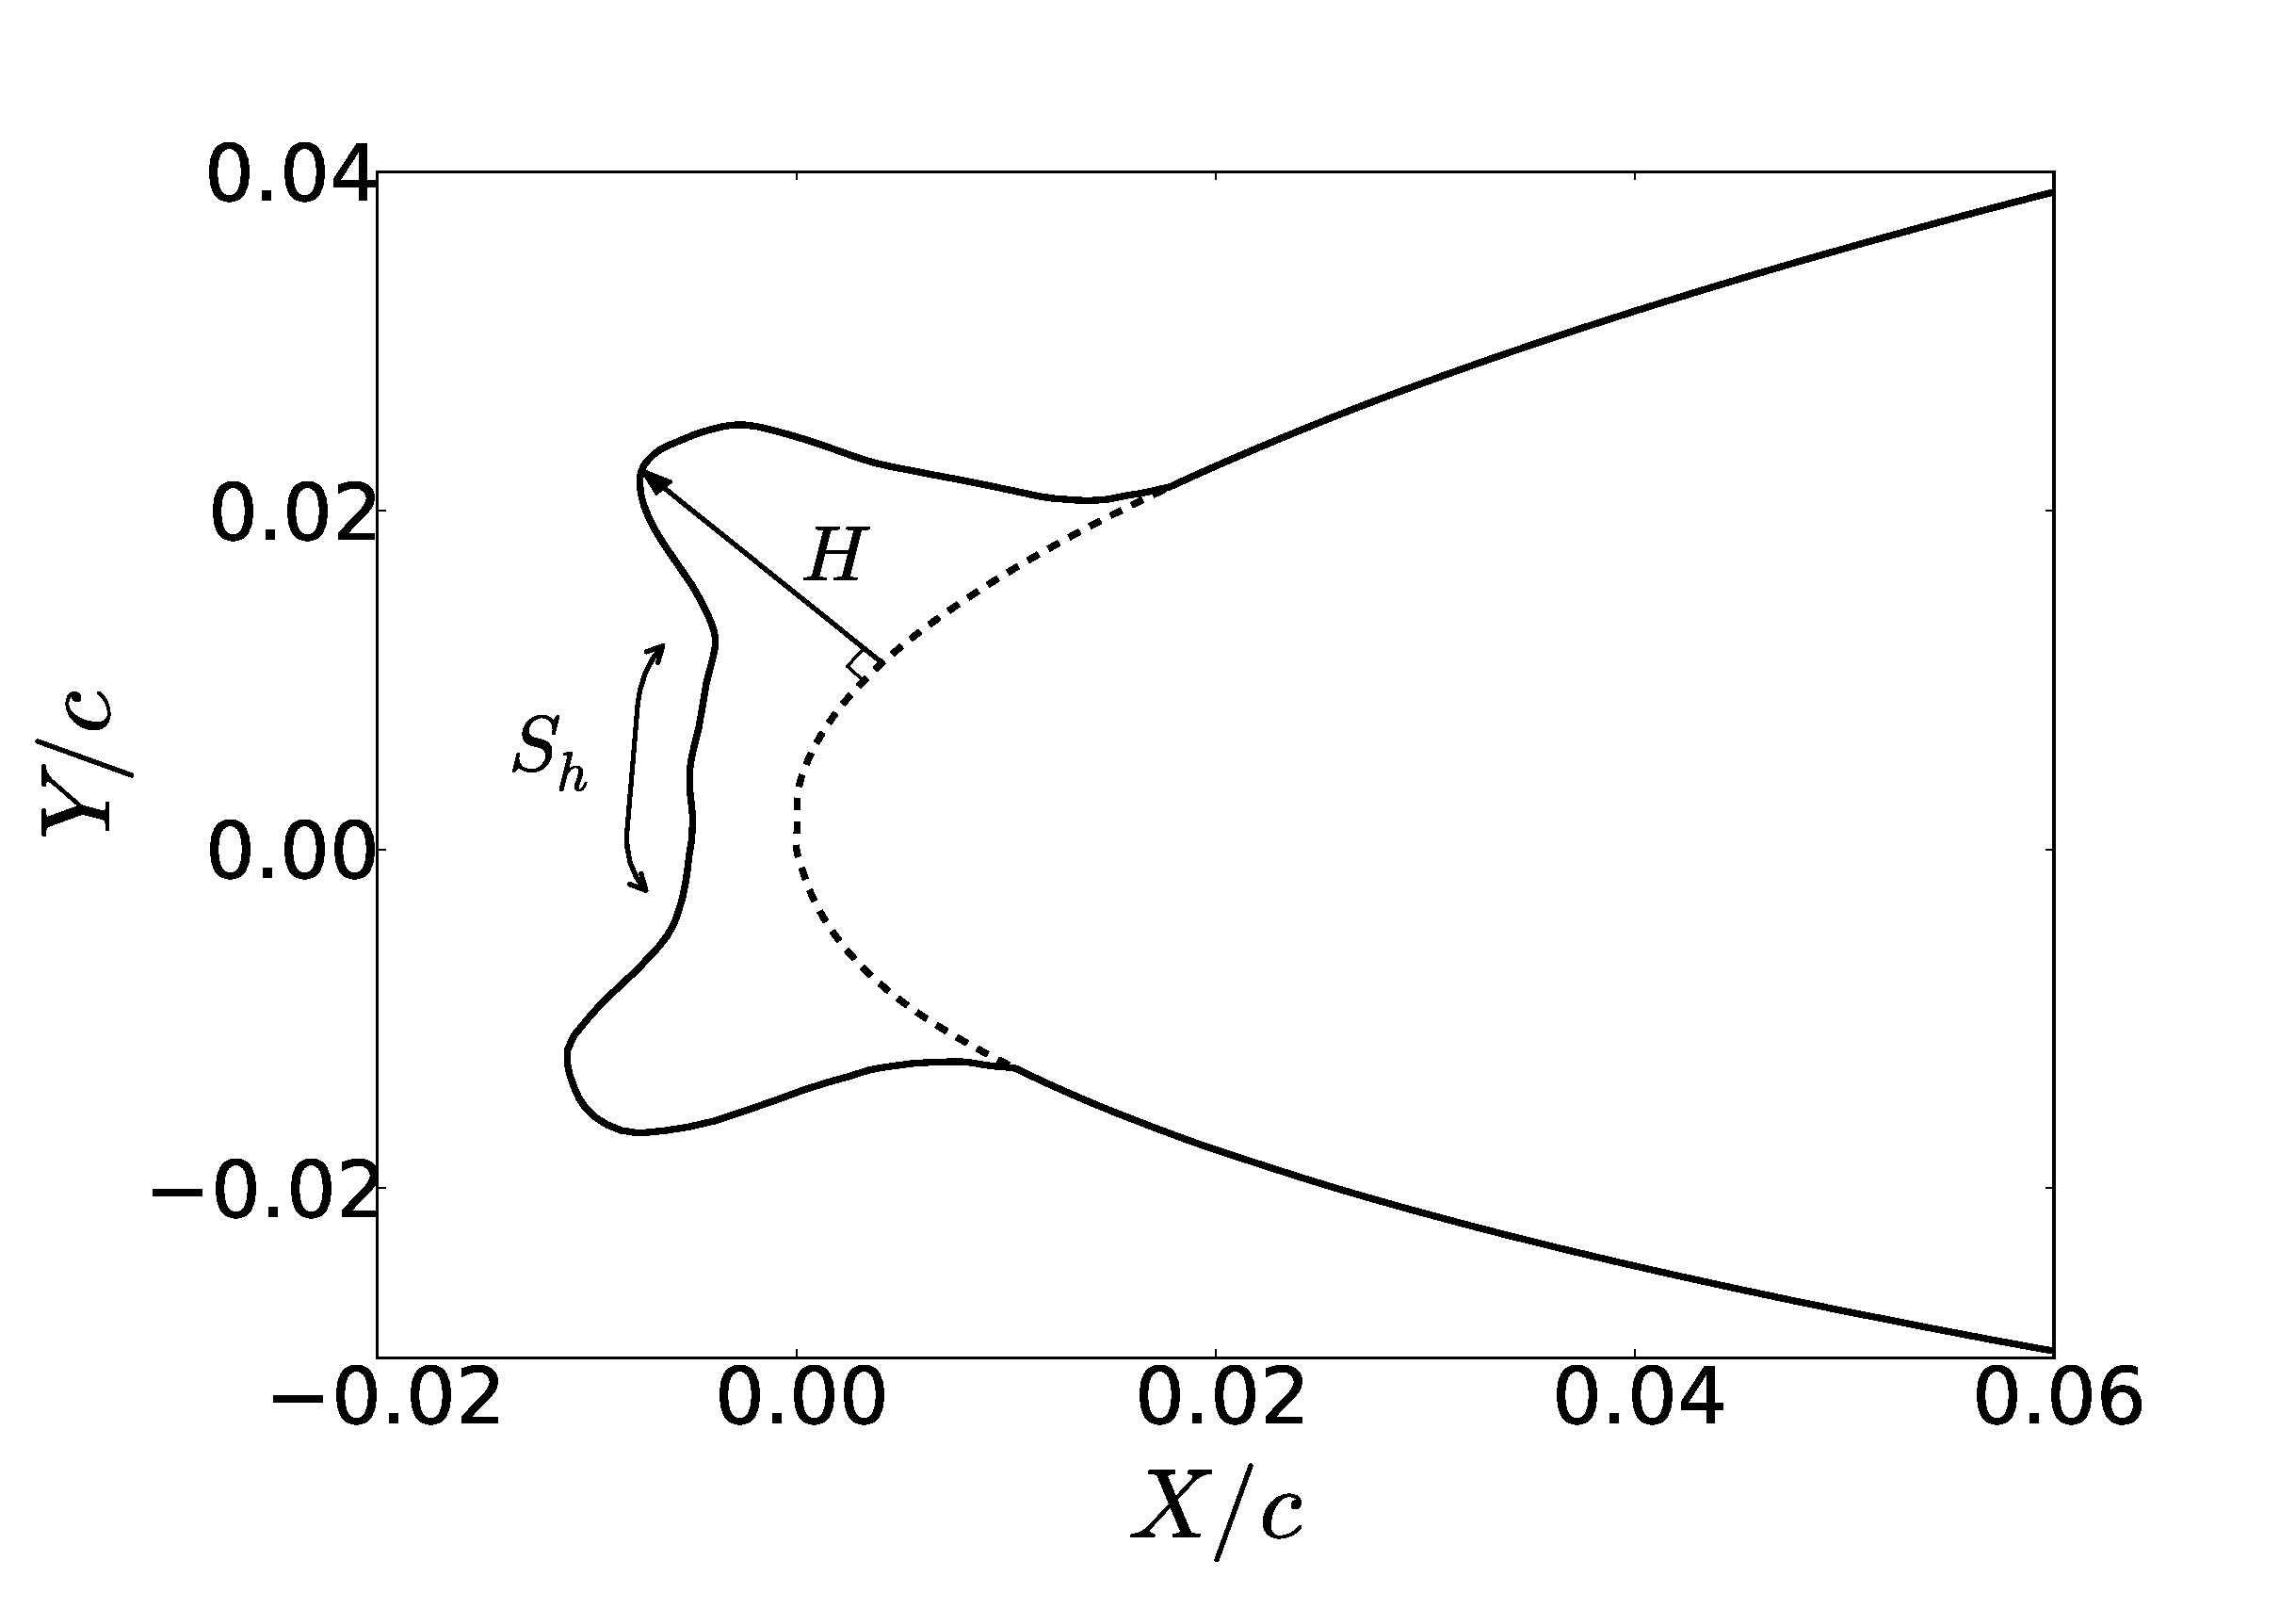
\includegraphics[width=0.95\textwidth]{NominalHorn}
\caption{Horn Ice}
\end{figure}
\vspace{-0.5cm}
\begin{itemize}
\item Forms in relatively warm conditions
\item Differential heat transfer rate
\end{itemize}
\end{minipage}
\end{frame}
\begin{frame}
\frametitle{Canonical Ice Shapes}
\label{sec-2-2}

\begin{itemize}
\item \textbf{Basic scalings/translations}\footnote{DeGennaro A., Rowley C.W., and Martinelli,
L. \emph{Uncertainty Quantification for Airfoil Icing using Polynomial Chaos Expansions}. Journal of Aircraft, 2015.
 }
\end{itemize}
\centering
\vspace{-0.5cm}
\begin{minipage}[t]{0.45\linewidth}
\begin{figure}[t]
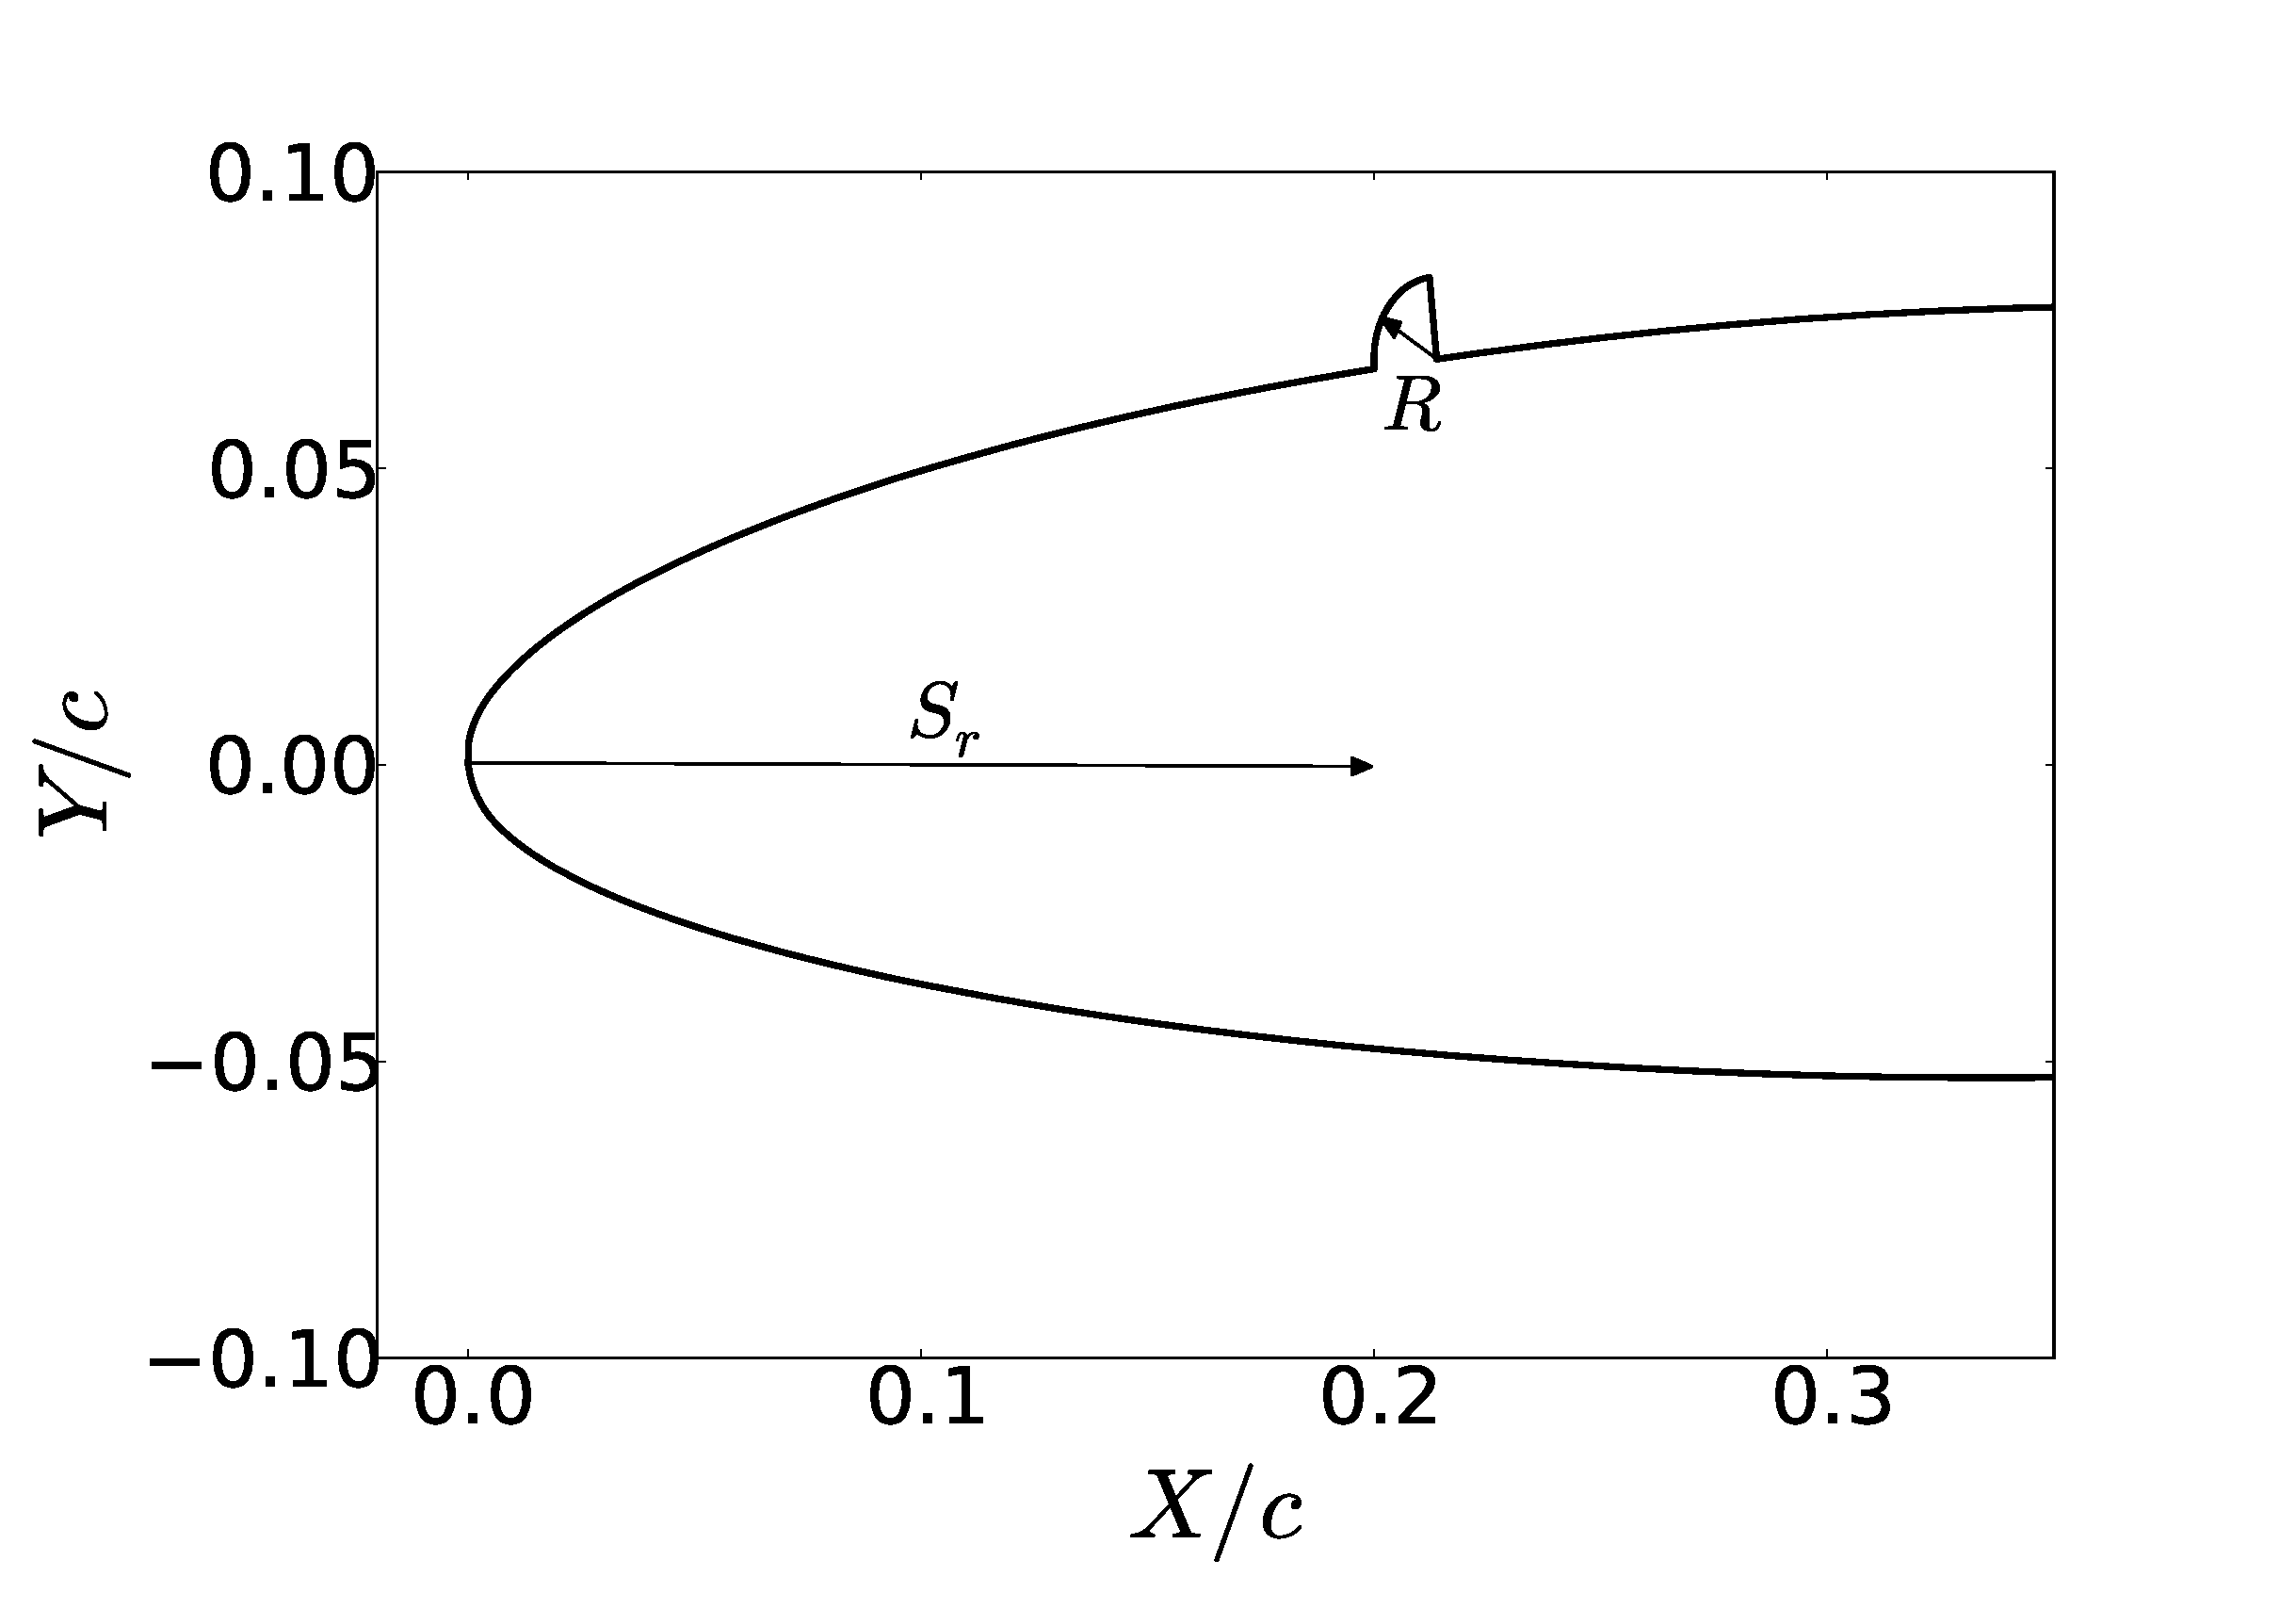
\includegraphics[width=0.95\textwidth]{RidgeParameters}
\caption{Ridge Parameterization}
\end{figure}
\vspace{-0.5cm}
\begin{itemize}
\item Ridge radius
\item Ridge position
\end{itemize}
\end{minipage}
\begin{minipage}[t]{0.45\linewidth}
\begin{figure}[t]
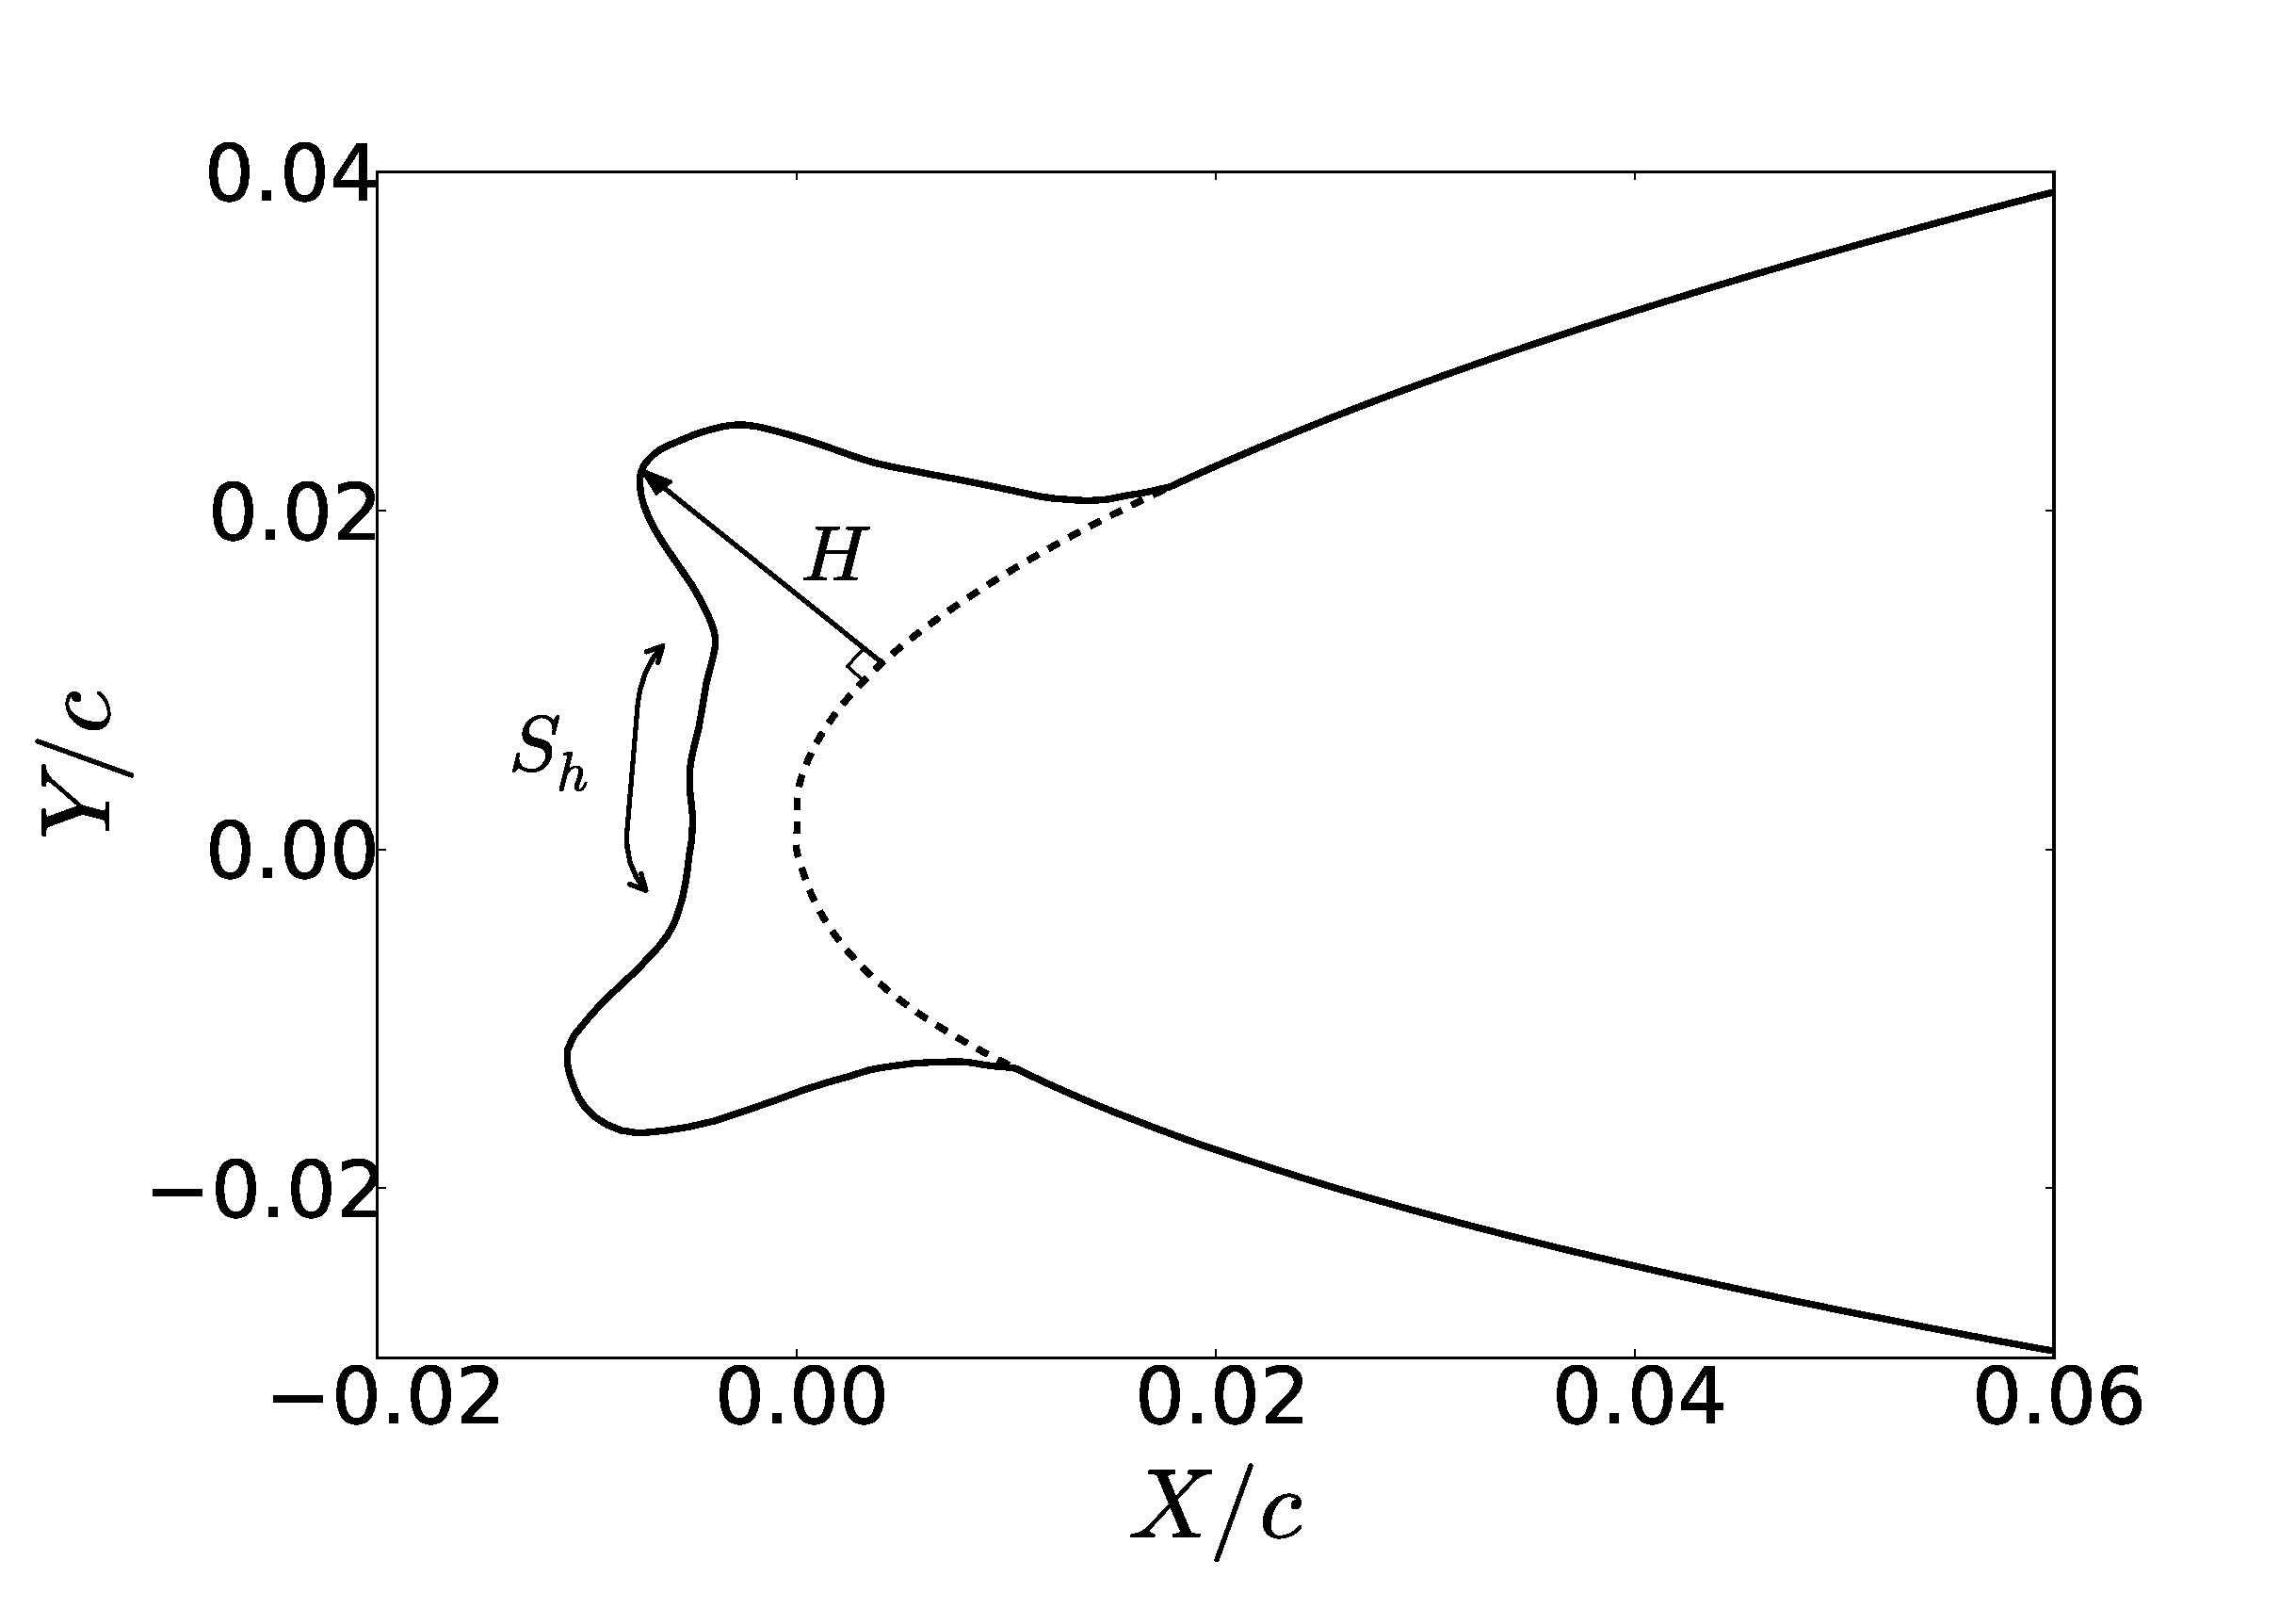
\includegraphics[width=0.95\textwidth]{NominalHorn}
\caption{Horn Parameterization}
\end{figure}
\vspace{-0.5cm}
\begin{itemize}
\item Horn height
\item Horn separation
\end{itemize}
\end{minipage}
\end{frame}
\begin{frame}
\frametitle{Application to Icing UQ}
\label{sec-2-3}

\begin{itemize}
\item We wish to apply a fast and accurate method for quantifying
  uncertainty in the aerodynamics of these ice shapes
\item Choose to use polynomial chaos expansions (PCE)
\begin{itemize}
\item Fast compared to Monte Carlo
\item Explicit surrogate
\item Easy statistical sampling
\item Can compute sensitivities, analysis of variance
\end{itemize}
\item We will compute UQ results for horn and ridge problems using PCE,
  and verify them against high-resolution Monte Carlo simulations
\end{itemize}
\end{frame}
\begin{frame}
\frametitle{Polynomial Chaos Expansions (PCE)}
\label{sec-2-4}


\begin{itemize}
\item \textbf{Polynomial Chaos Framework} \footnote{Xiu D. \emph{Numerical Methods for Stochastic Computations: A Spectral Method Approach}. Princeton University Press, 2010.
 }
\begin{itemize}
\item Let $\bv{Z} = (Z_1 \ldots Z_d)$ be $d$ random variables with PDF
    $\rho(\bv{Z})$ that parameterize ice
\item Let $\lbrace \Phi_k \rbrace$ denote the set of polynomials
    which are orthogonal w.r.t. $\rho(\bv{Z})$
\item Let $y(\bv{Z})$ denote the mapping from $\bv{Z}$ to an aerodynamic
    performance metric
\end{itemize}
\item \textbf{Probabilistic Collocation Method:}
\begin{itemize}
\item \emph{Representation} 
    \begin{equation*}
      y(\bv{Z}) \approx \sum_{|i|=0}^N y_i \Phi_i(\bv{Z})
    \end{equation*}
\item \emph{Orthonormality} 
    \begin{equation*}
    \begin{aligned}
      \ip{f}{g} &= \int_{\Gamma} f(\bv{z})g(\bv{z}) \rho(\bv{z}) d\bv{z} \\
      \ip{\Phi_i}{\Phi_j} &= \delta_{ij}
    \end{aligned}
    \end{equation*}
\item \emph{Quadrature} 
    \begin{equation*}
      y_k = \ip{y}{\Phi_k} \approx \sum_{i=0}^{Q}
    y(\bv{Z}^{(k)}) \Phi_k(\bv{Z}^{(k)}) w_k
    \end{equation*}
\end{itemize}
\end{itemize}
\end{frame}
\begin{frame}
\frametitle{PCE Collocation}
\label{sec-2-5}

\begin{columns}[c]
  \column{0.7\textwidth}
    \centering
    \begin{figure}
    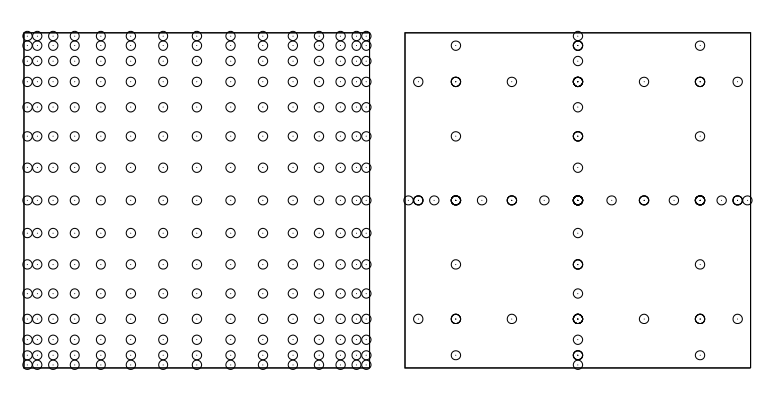
\includegraphics[width=0.95\textwidth]{SparseGrid1}
    \caption{Full Tensor Product vs. Sparse Grid}
    \end{figure}
  \column{0.3\textwidth}
    \centering
    \begin{figure}
    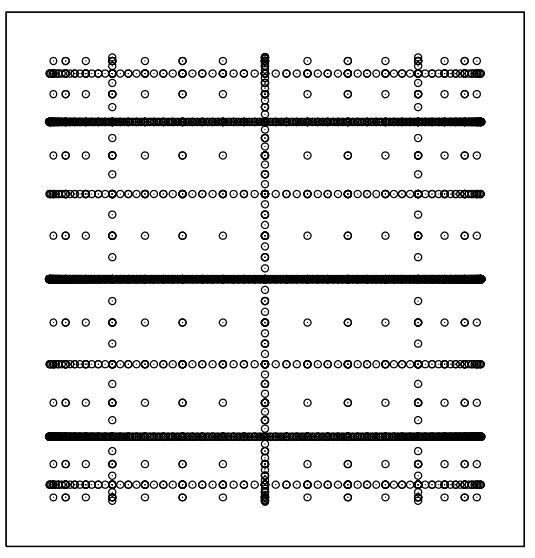
\includegraphics[width=0.95\textwidth]{SparseGrid2} \\
    \caption{Anisotropic Grid}
    \end{figure}
\end{columns}

\begin{itemize}
\item Full tensor grids can be used when probability space is low-dimensional
\item Sparse grids can be used otherwise\footnote{LeMaitre O. \emph{Spectral Methods for Uncertainty Quantification}. Springer, 2010.
 }
\end{itemize}
\end{frame}
\begin{frame}
\frametitle{Application to Icing UQ}
\label{sec-2-6}

\begin{itemize}
\item Parameterize shape variation for ridge/horn
\begin{itemize}
\item 2 parameters, equip with a distribution
\end{itemize}
\item Apply polynomial chaos methodology
\begin{itemize}
\item Full tensor grid sampling
\item 4$^{th}$-order polynomials --> $5\times5$ collocation mesh
\end{itemize}
\item Compute aerodynamics of resulting shapes
\begin{itemize}
\item In-house 2D steady-state RANS solver + hyperbolic mesh generator
\end{itemize}
\item Compare results against 500 Quasi-Monte Carlo samples
\end{itemize}
\end{frame}
\begin{frame}
\frametitle{Ridge Study}
\label{sec-2-7}

\centering
\vspace{-0.5cm}
\begin{minipage}[t]{0.45\linewidth}
\begin{figure}[t]
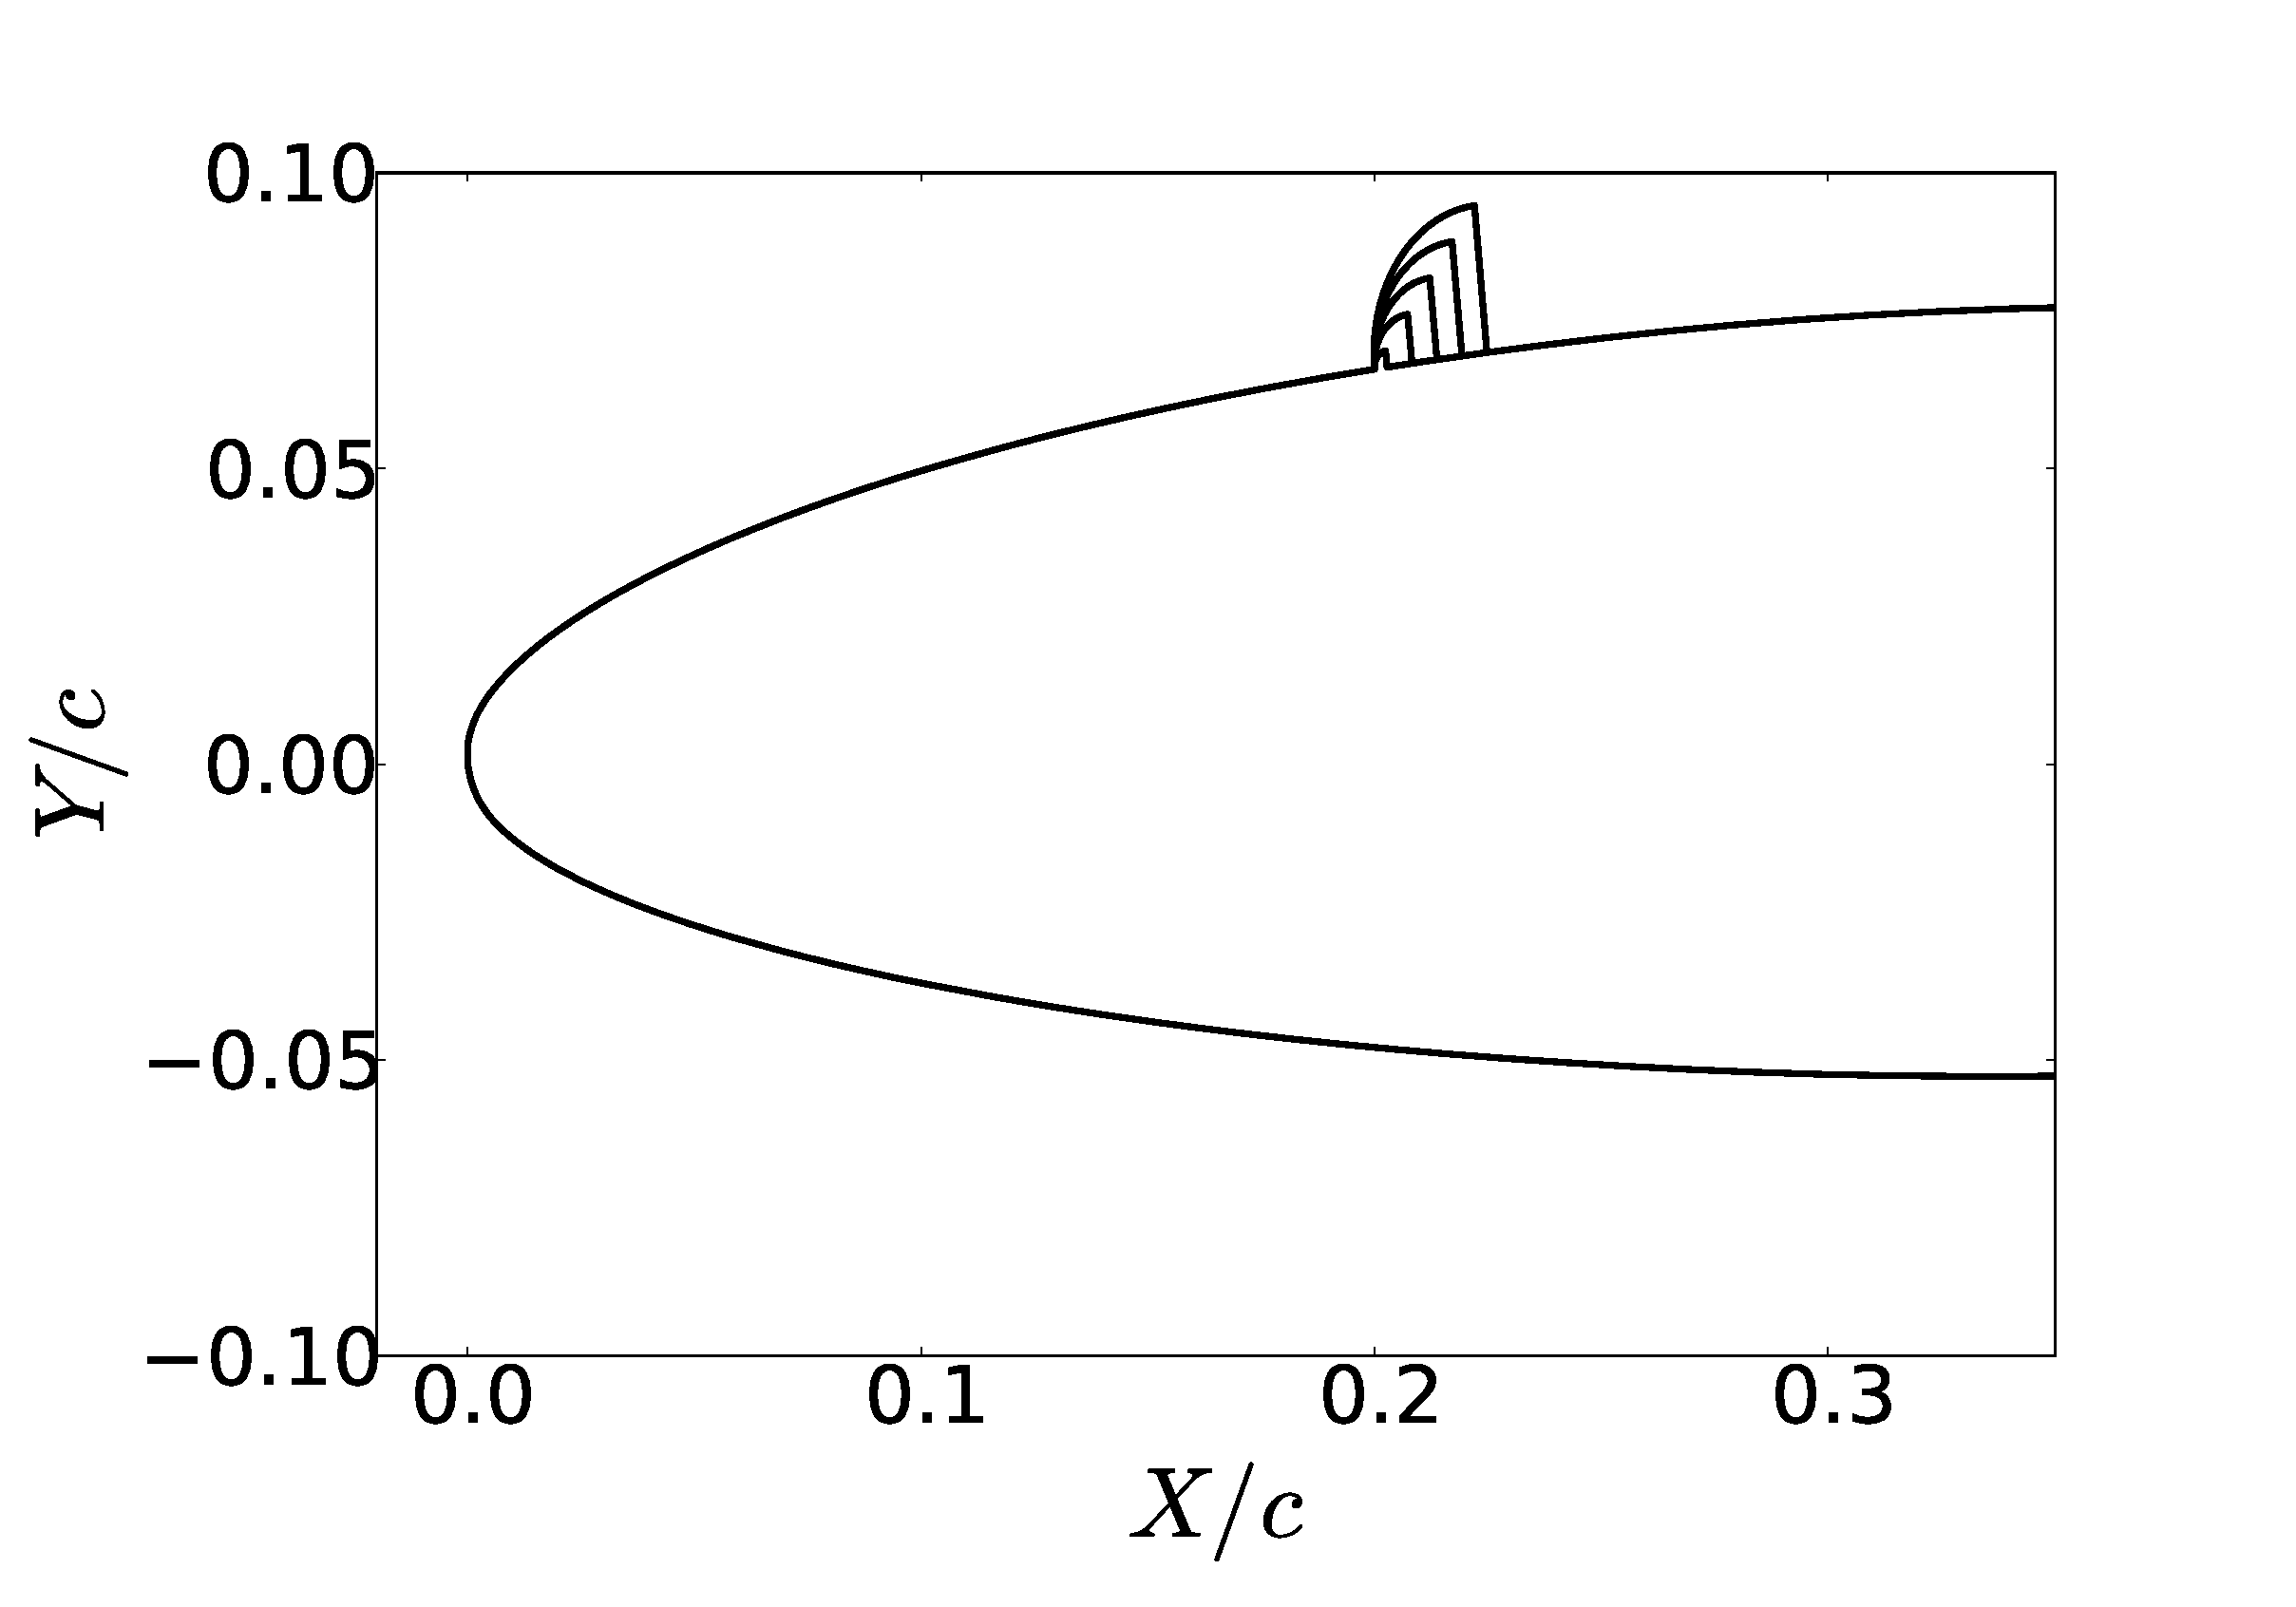
\includegraphics[width=0.75\textwidth]{RidgeRVariation}
\end{figure}
\vspace{-0.5cm}
\begin{figure}[t]
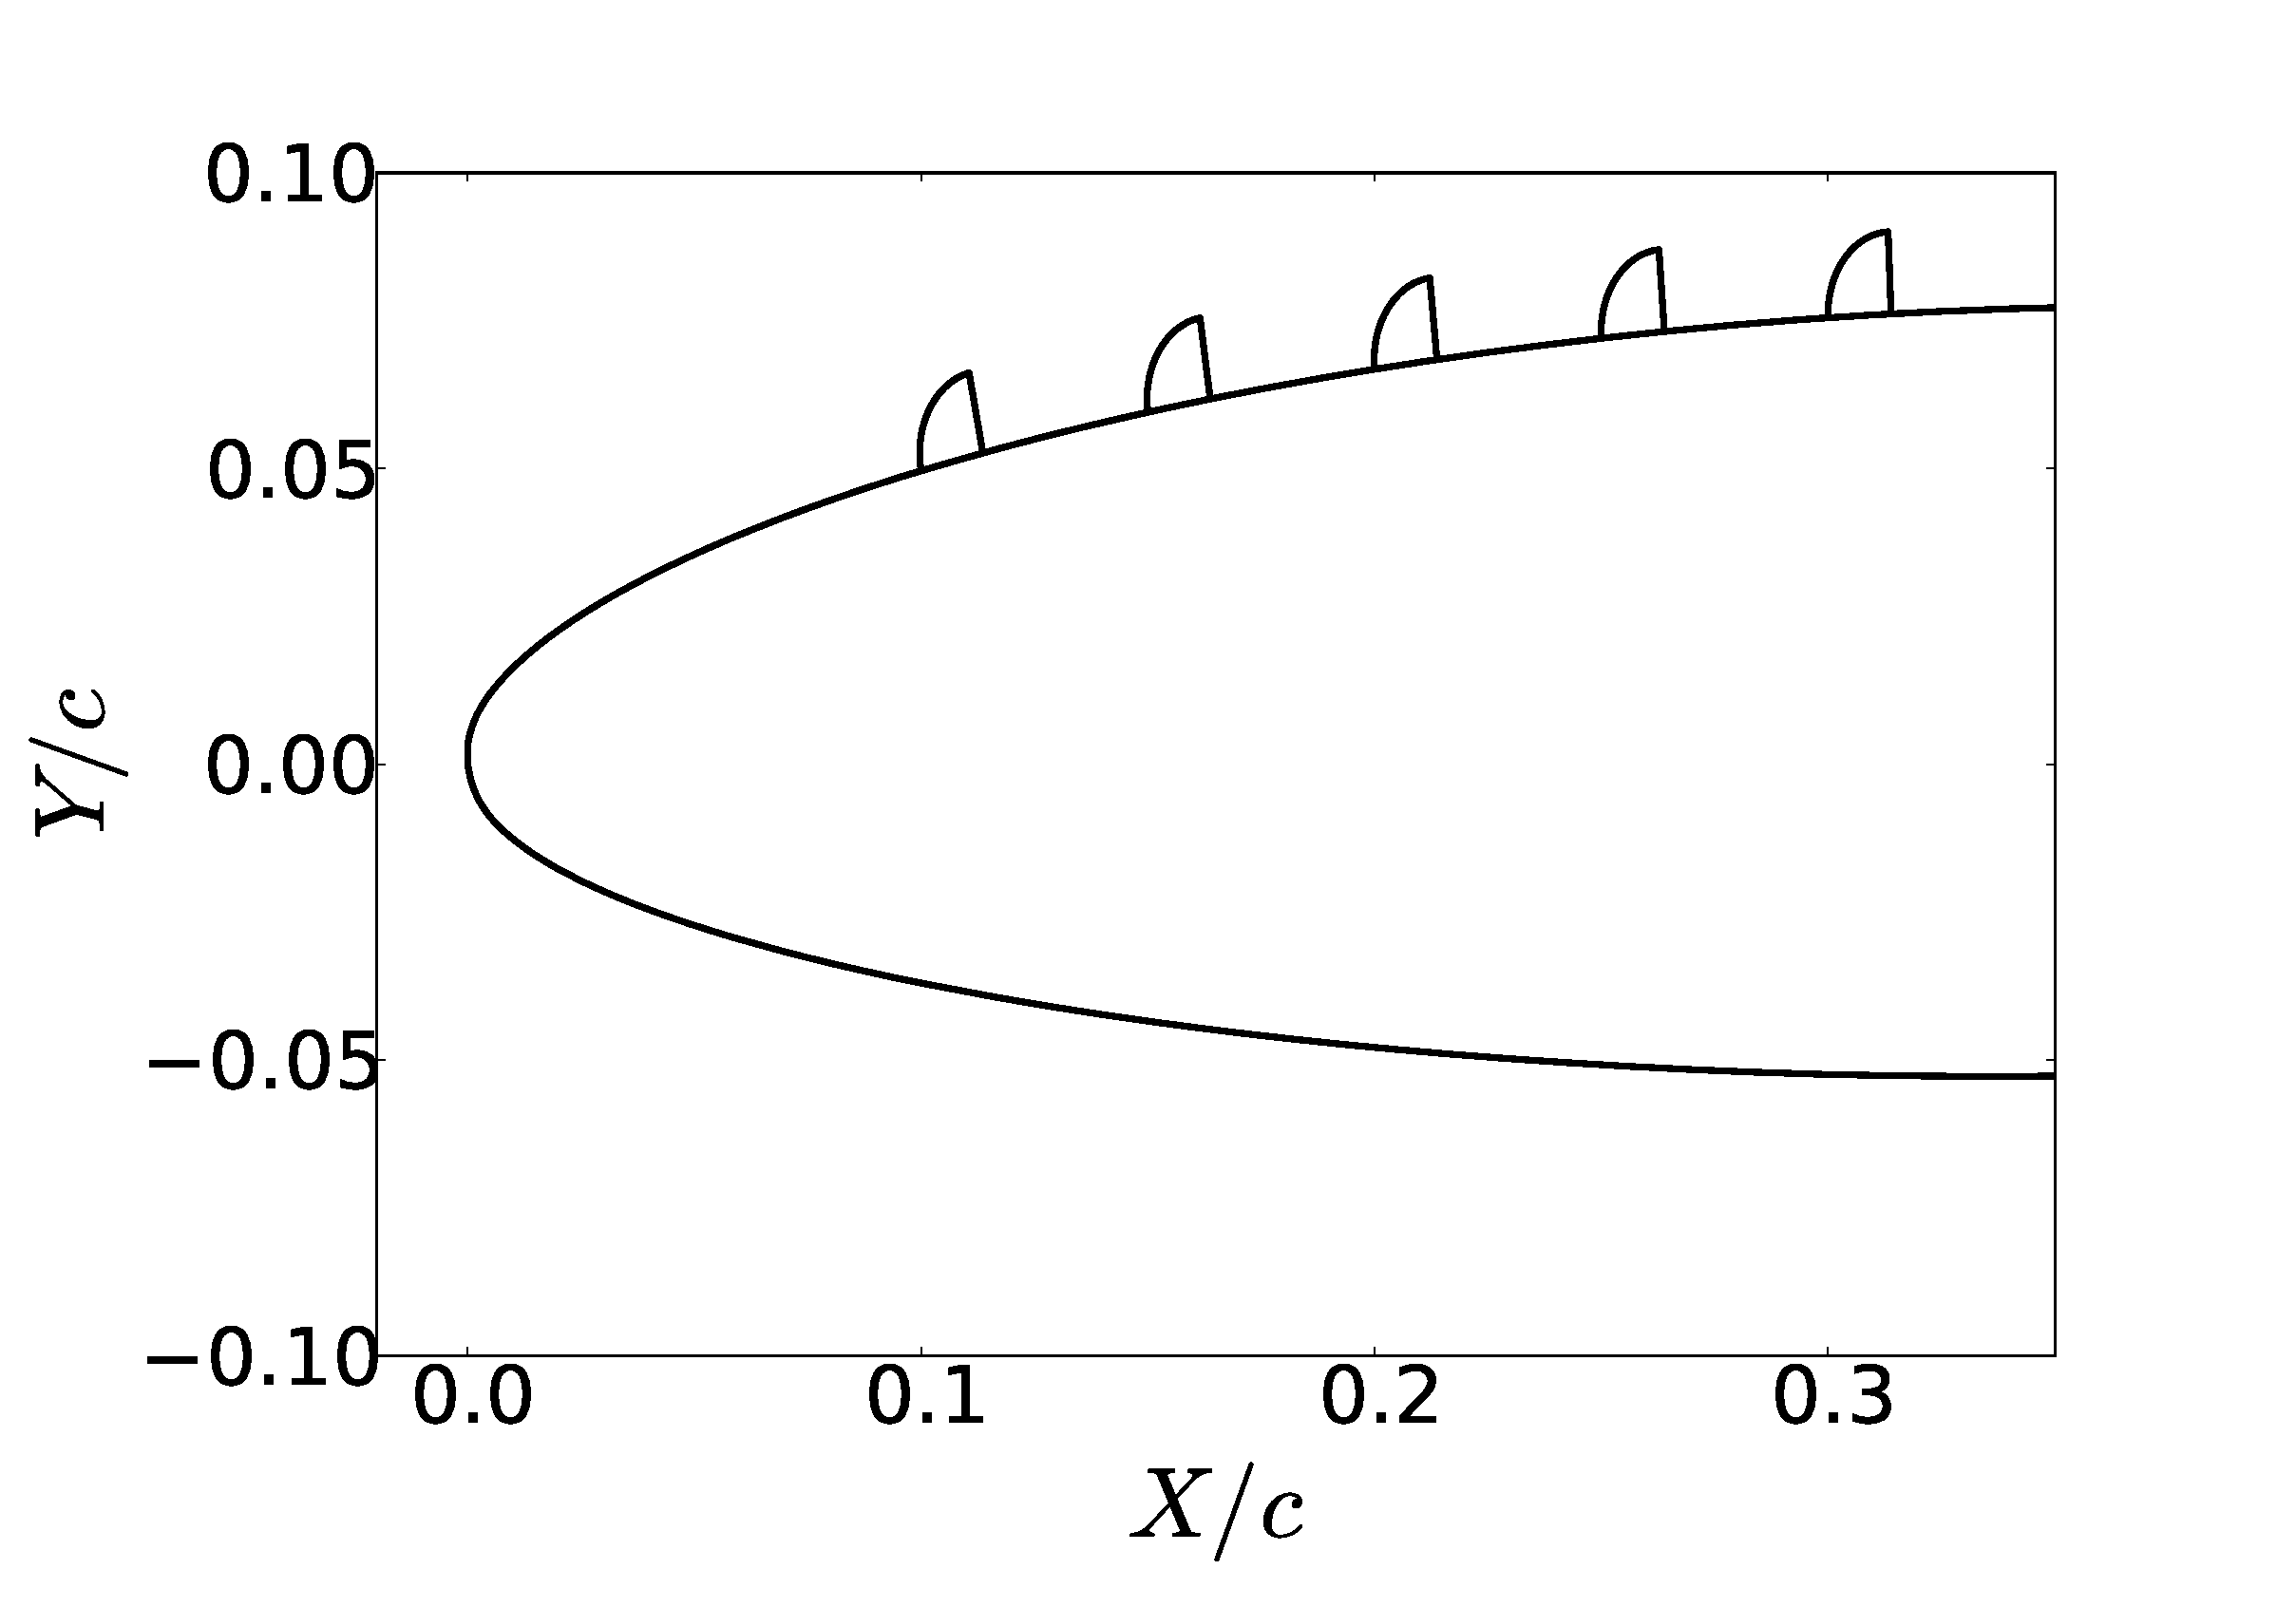
\includegraphics[width=0.75\textwidth]{RidgeSVariation}
\caption{Ridge Variations}
\end{figure}
\vspace{-0.5cm}
\end{minipage}
\begin{minipage}[t]{0.45\linewidth}
\begin{figure}[t]
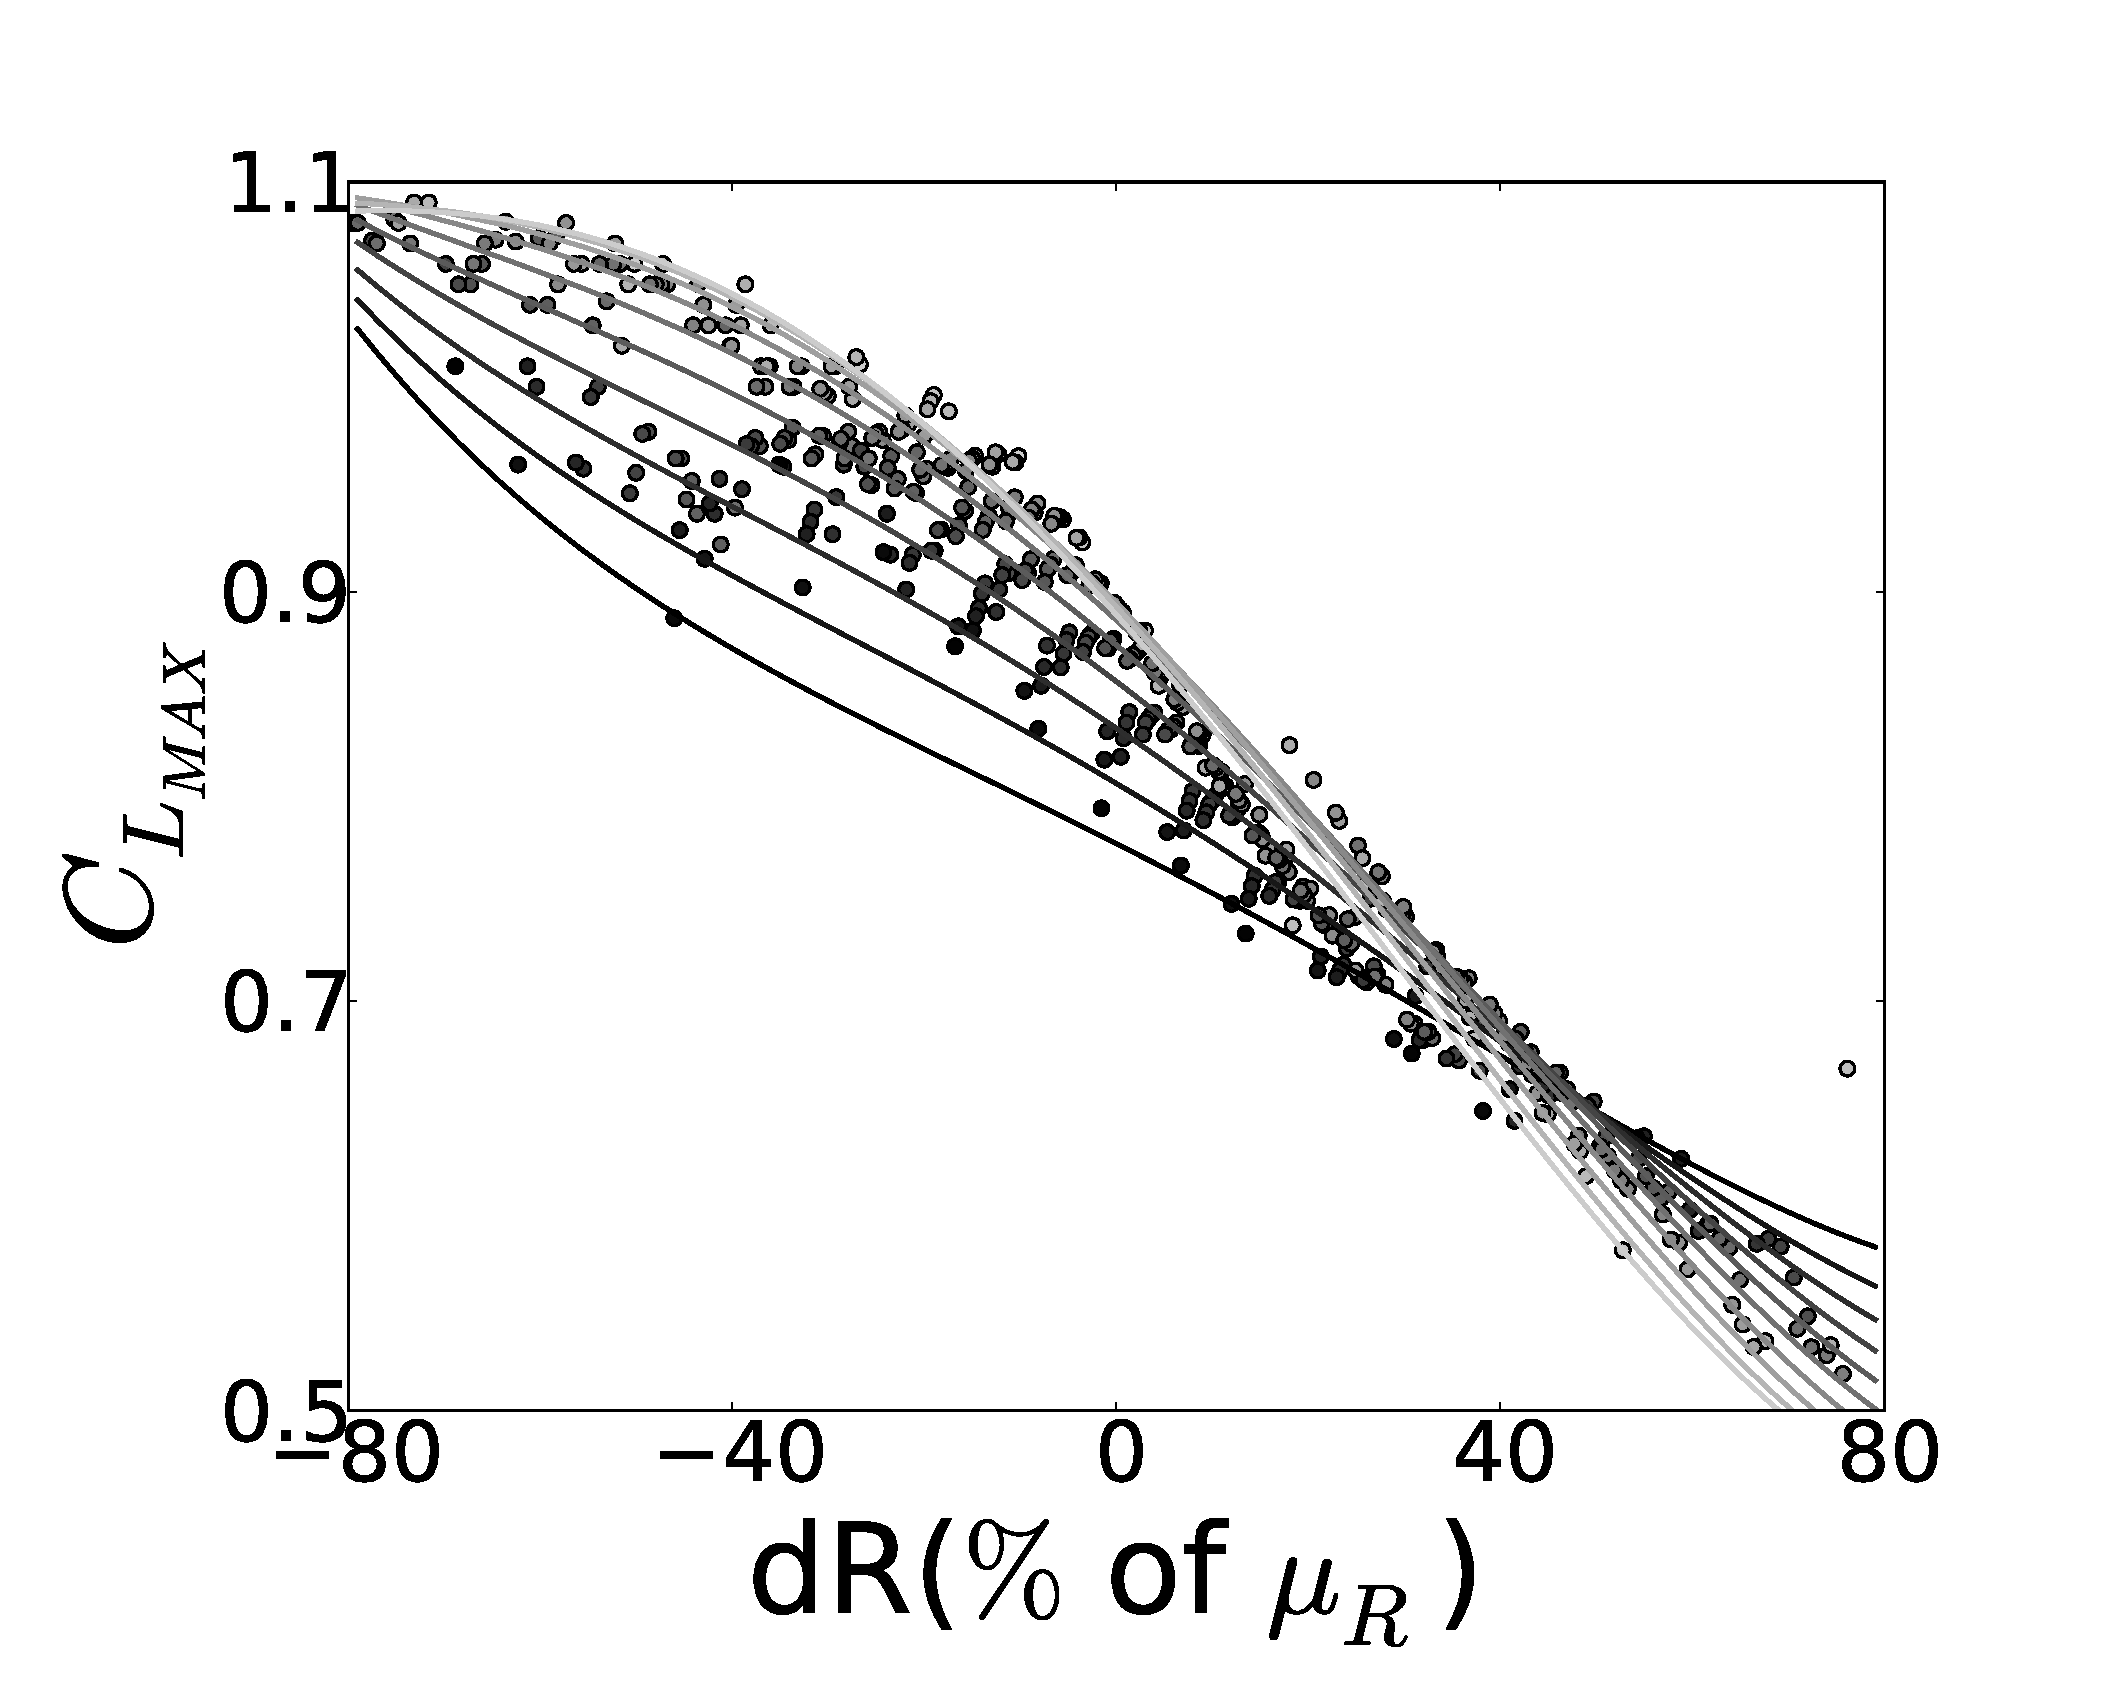
\includegraphics[width=0.65\textwidth]{MC_surrogate_LargeUnc_CL}
\end{figure}
\vspace{-0.6cm}
\begin{figure}[t]
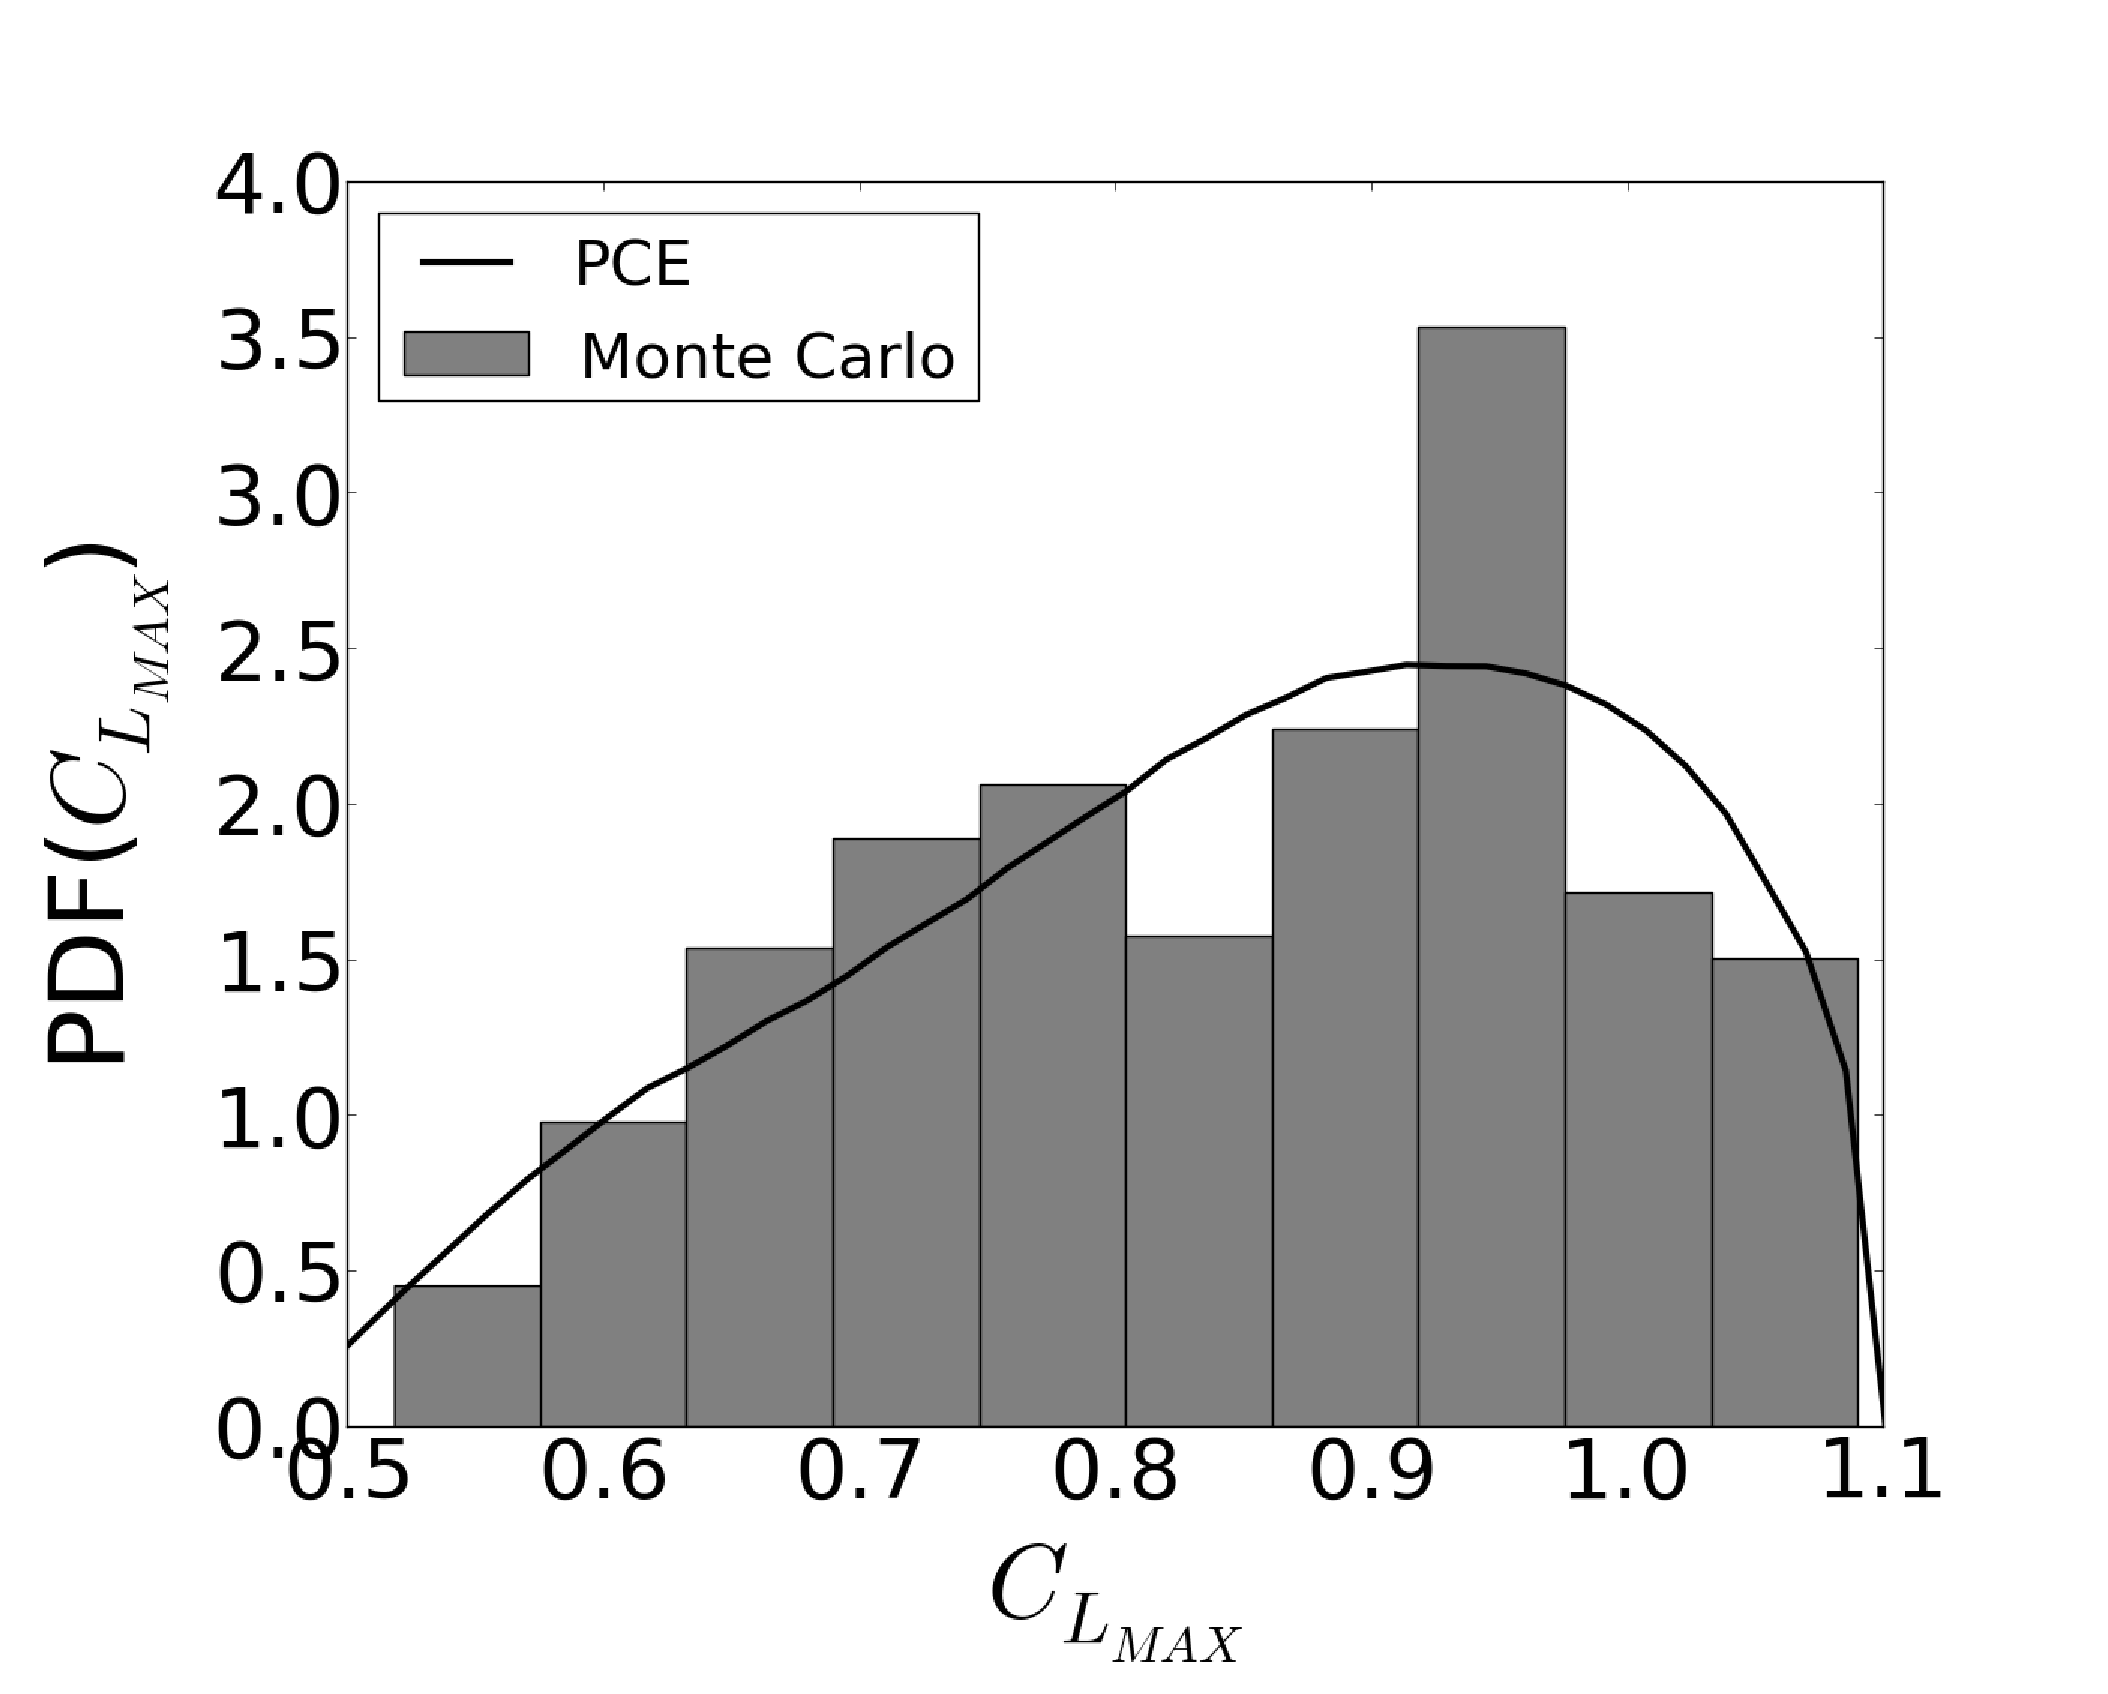
\includegraphics[width=0.65\textwidth]{MCgpcPDFLargeUnc_CL}
\caption{Lift Statistics}
\end{figure}
\end{minipage}
\begin{itemize}
\item Ridge parameters normally distributed about mean
\item Performance degrades with larger size, closer to L.E.
\end{itemize}
\end{frame}
\begin{frame}
\frametitle{Horn Study}
\label{sec-2-8}

\centering
\vspace{-0.5cm}
\begin{minipage}[t]{0.45\linewidth}
\begin{figure}[t]
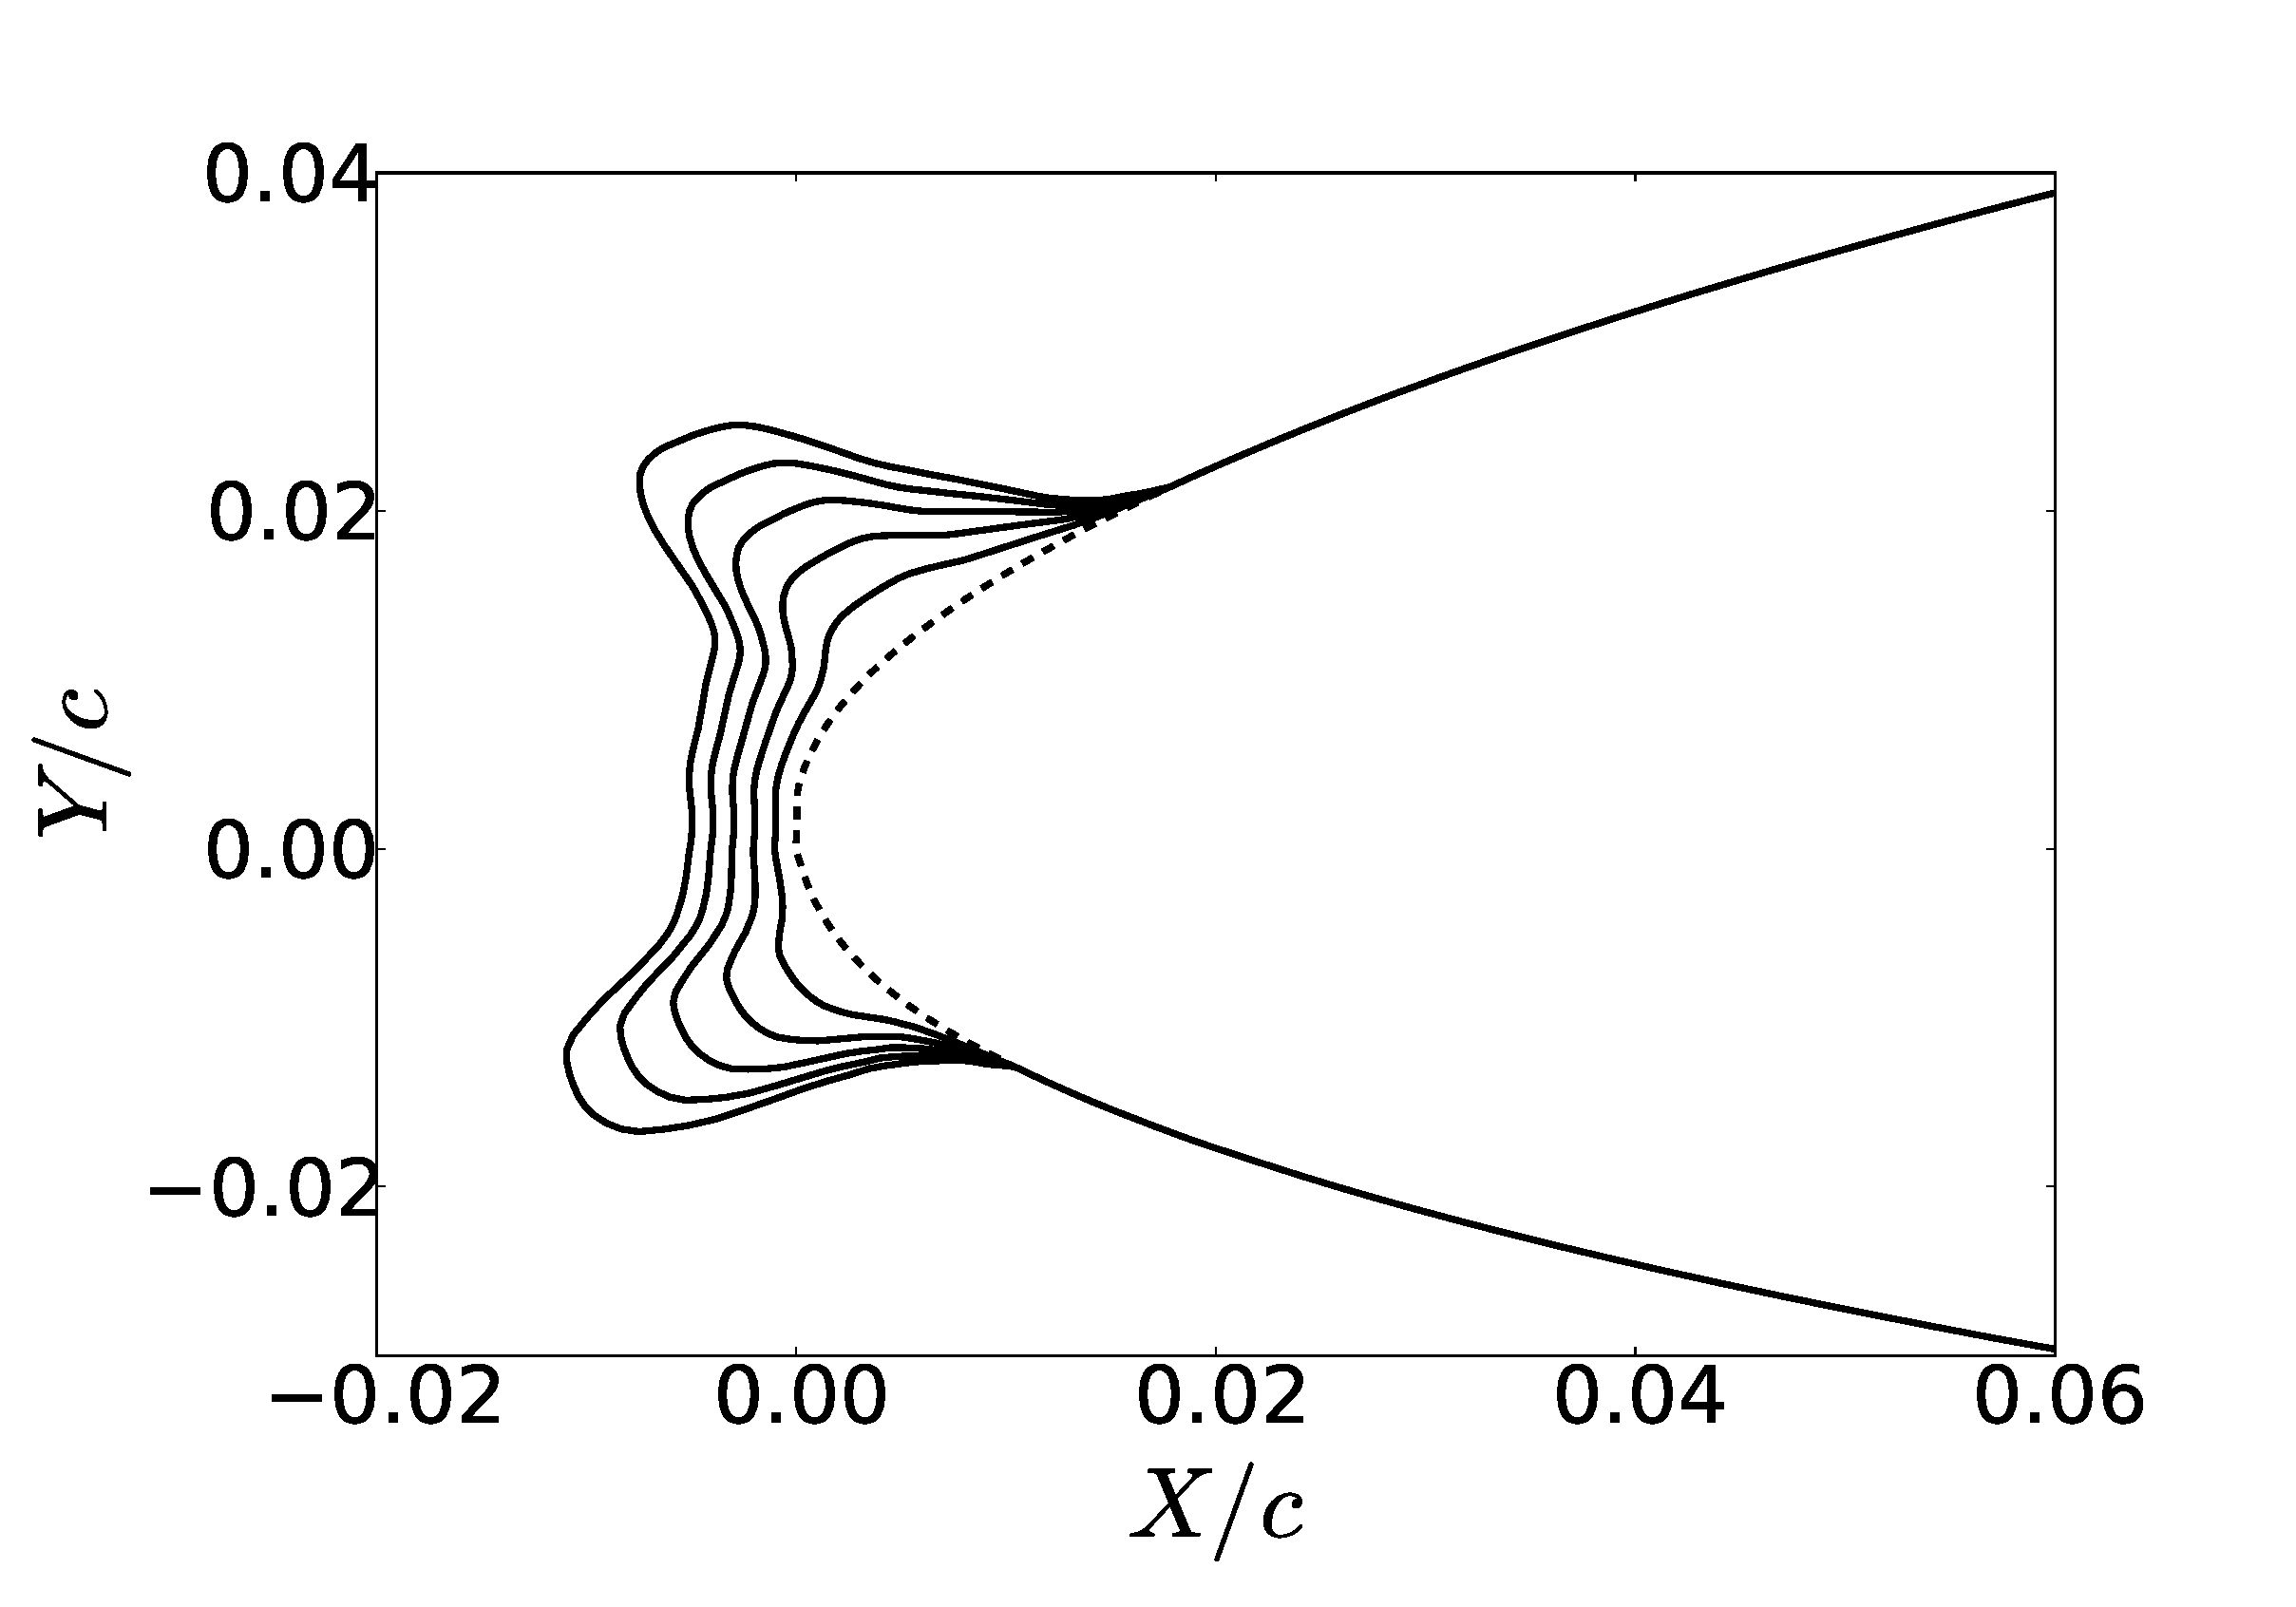
\includegraphics[width=0.75\textwidth]{HornHVariation}
\end{figure}
\vspace{-0.5cm}
\begin{figure}[t]
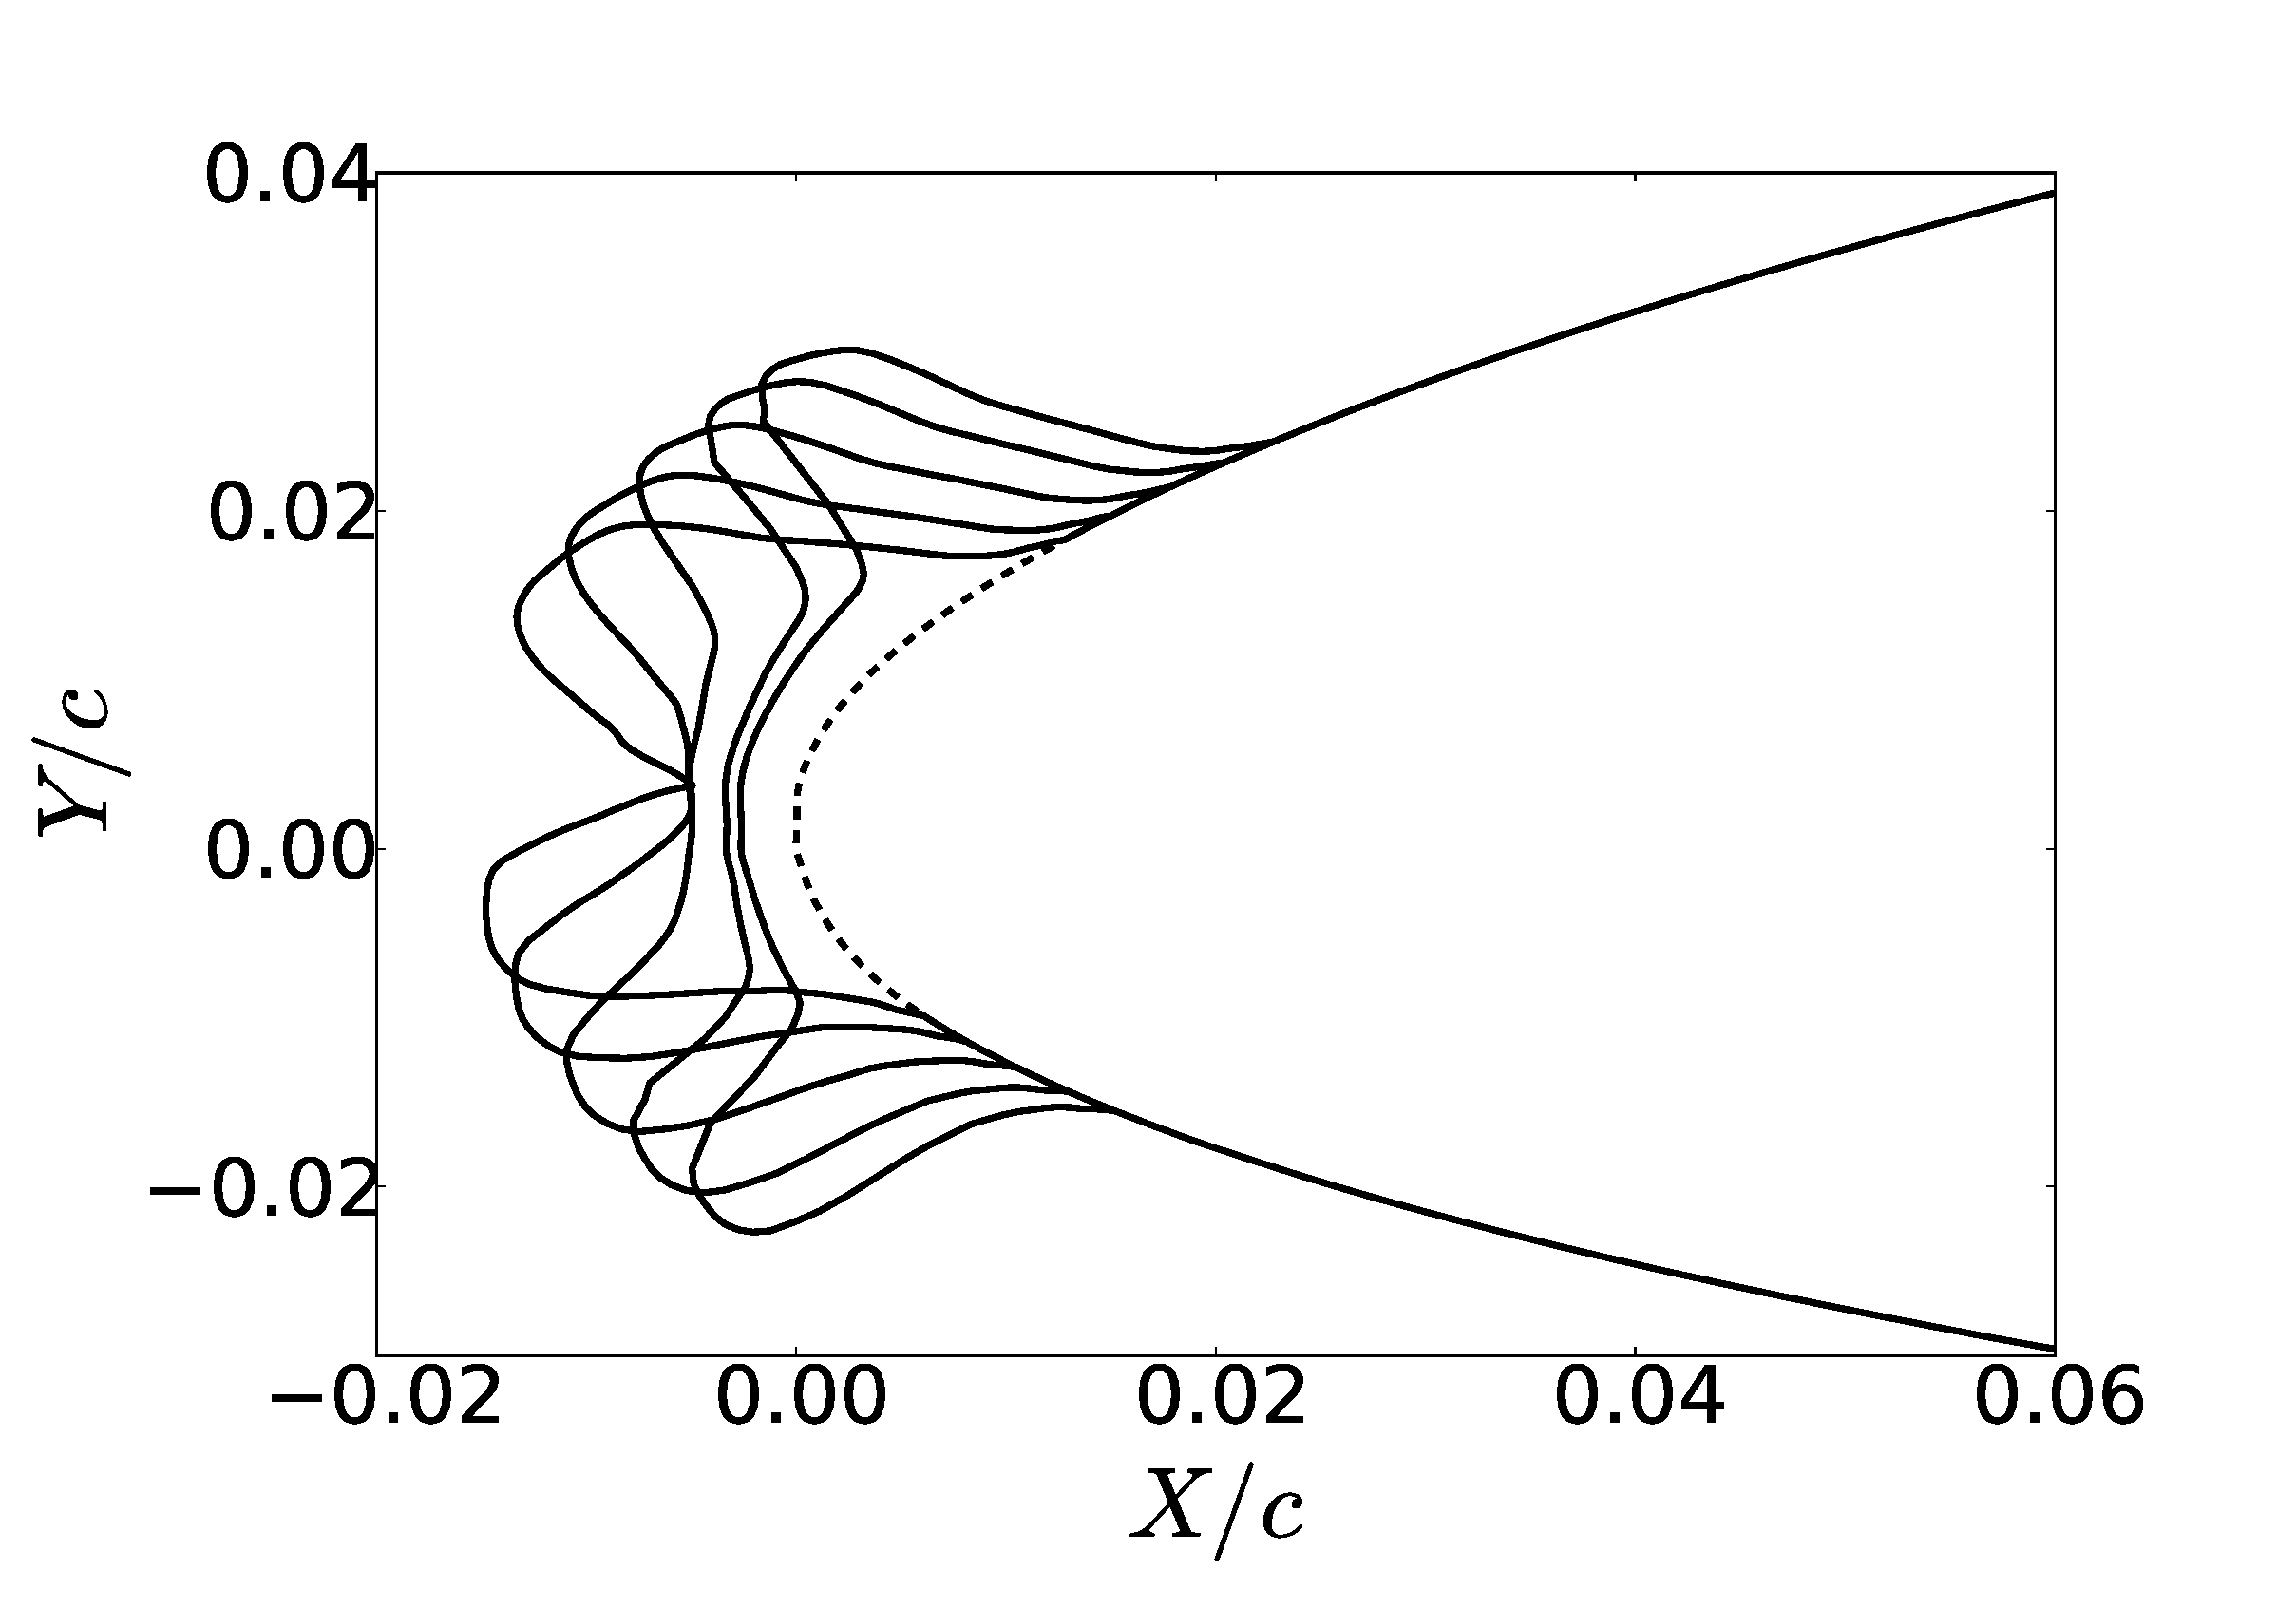
\includegraphics[width=0.75\textwidth]{HornSVariation}
\caption{Ridge Variations}
\end{figure}
\vspace{-0.5cm}
\end{minipage}
\begin{minipage}[t]{0.45\linewidth}
\begin{figure}[t]
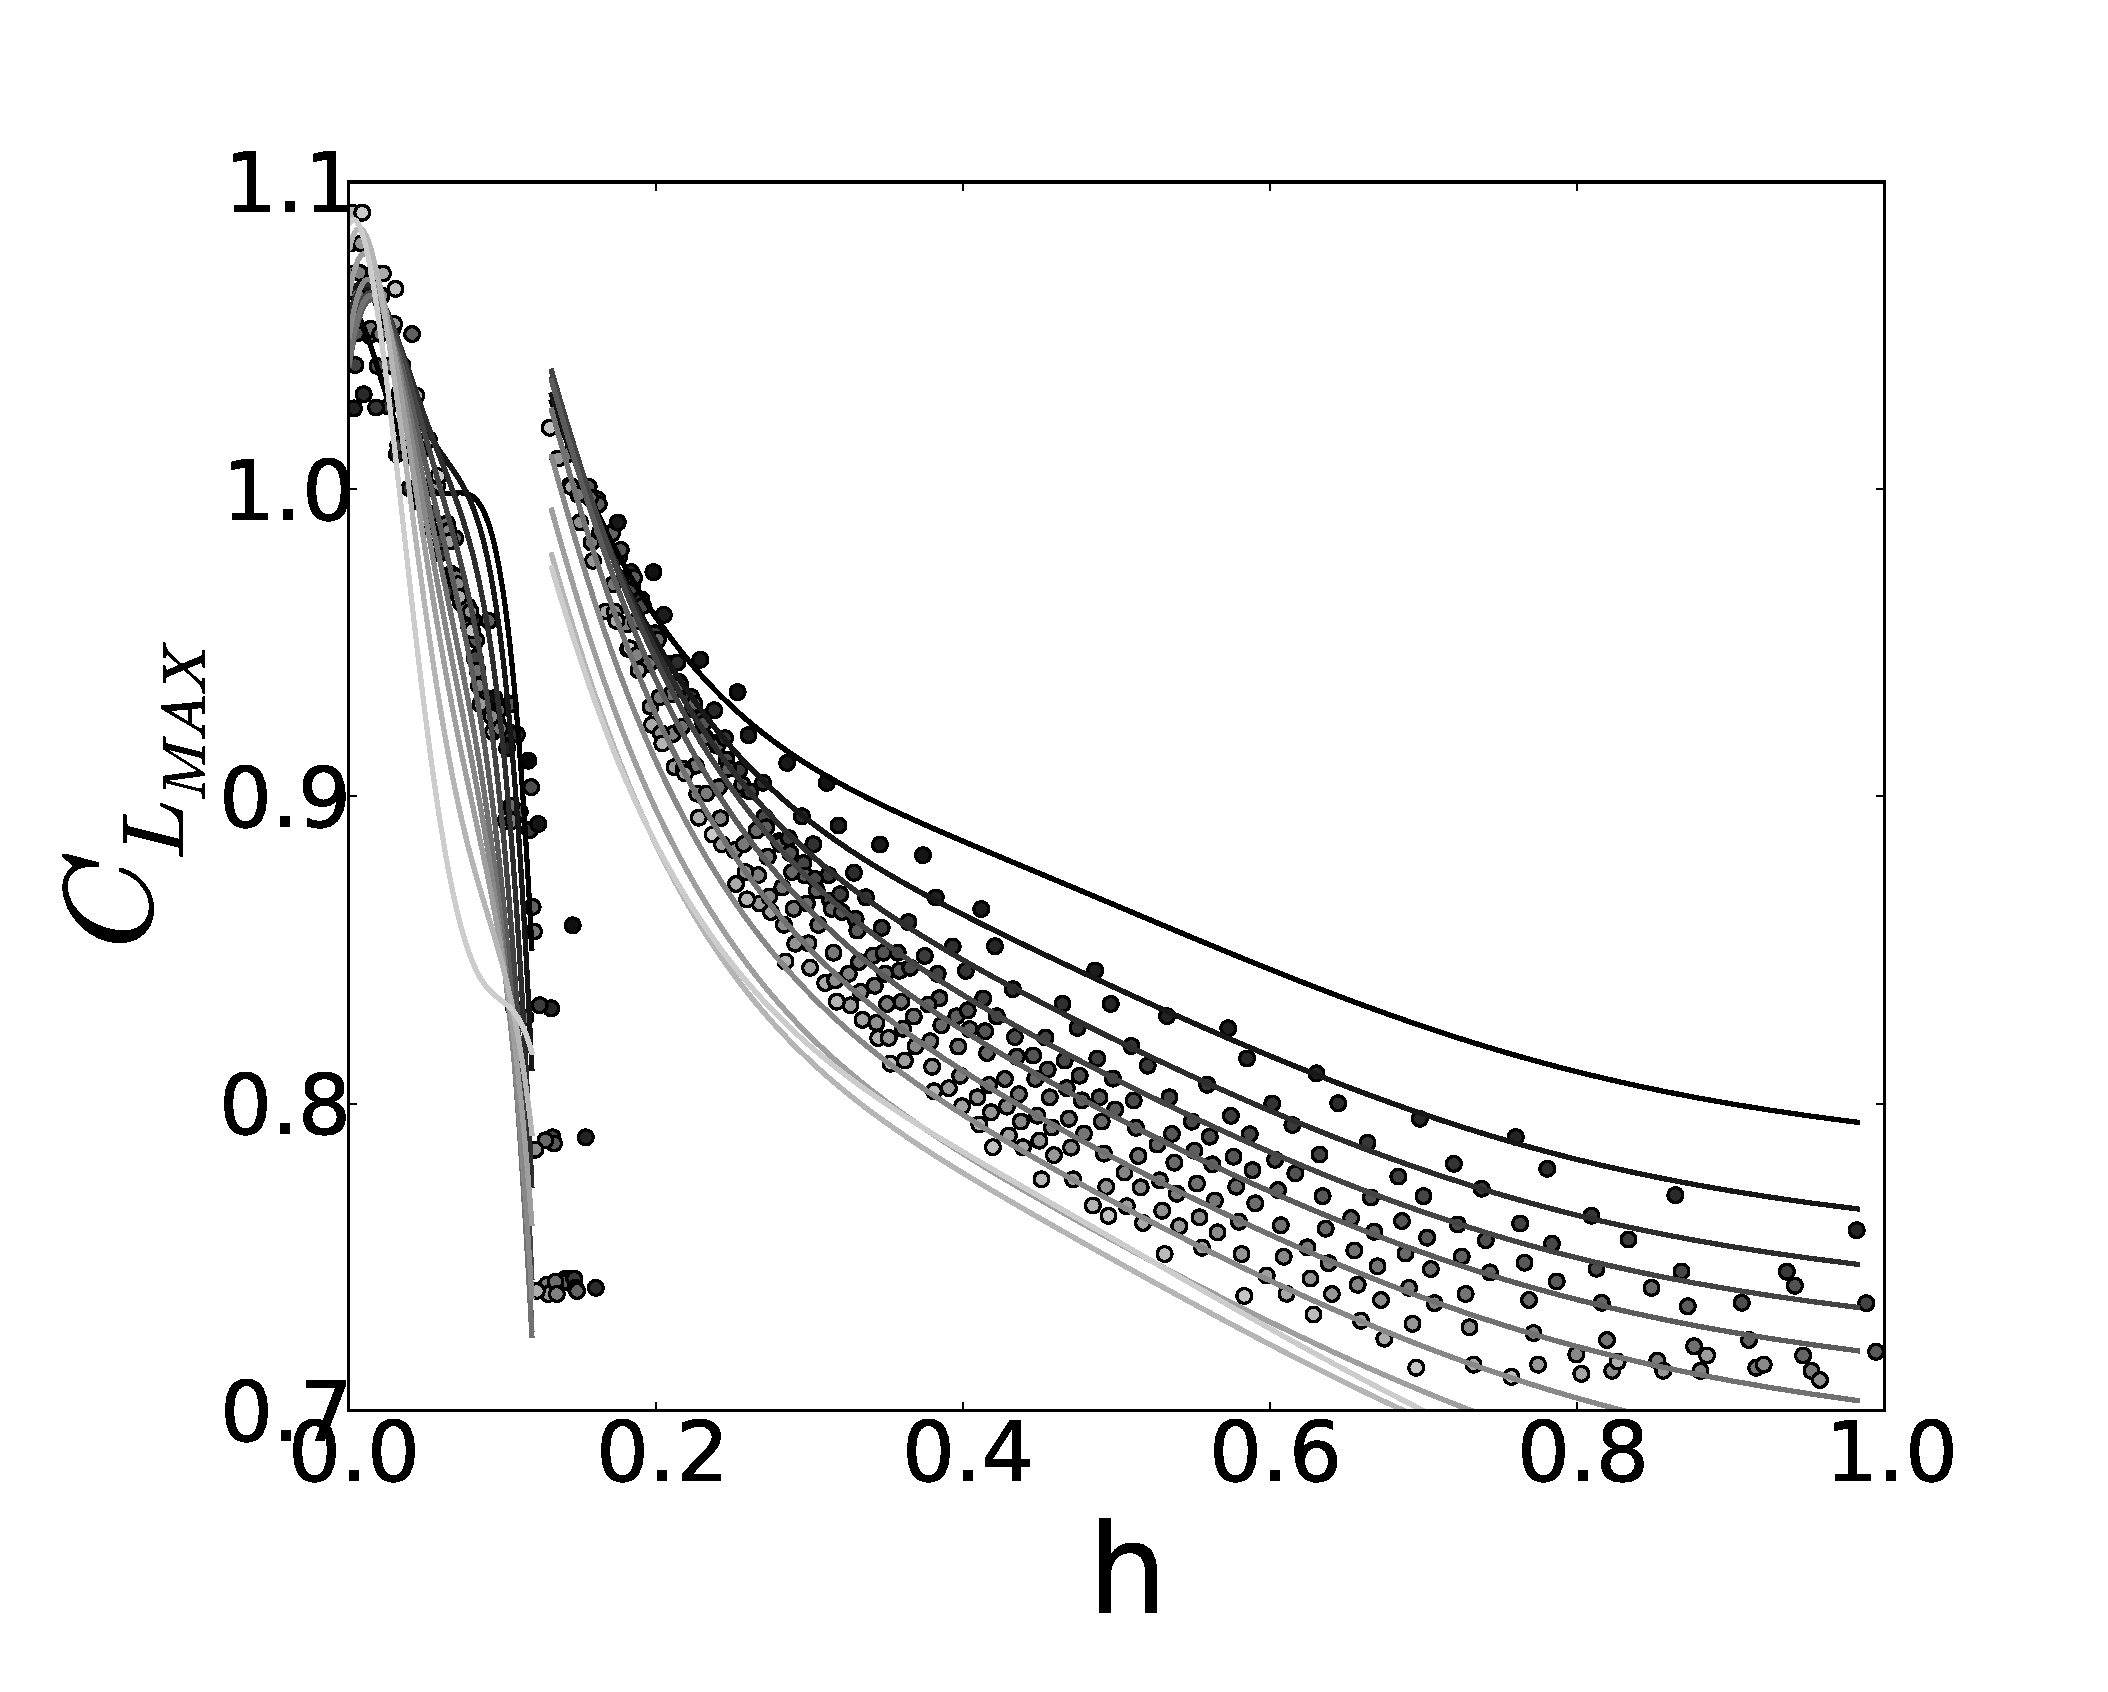
\includegraphics[width=0.65\textwidth]{CLMAX_MEGPCHORN}
\end{figure}
\vspace{-0.6cm}
\begin{figure}[t]
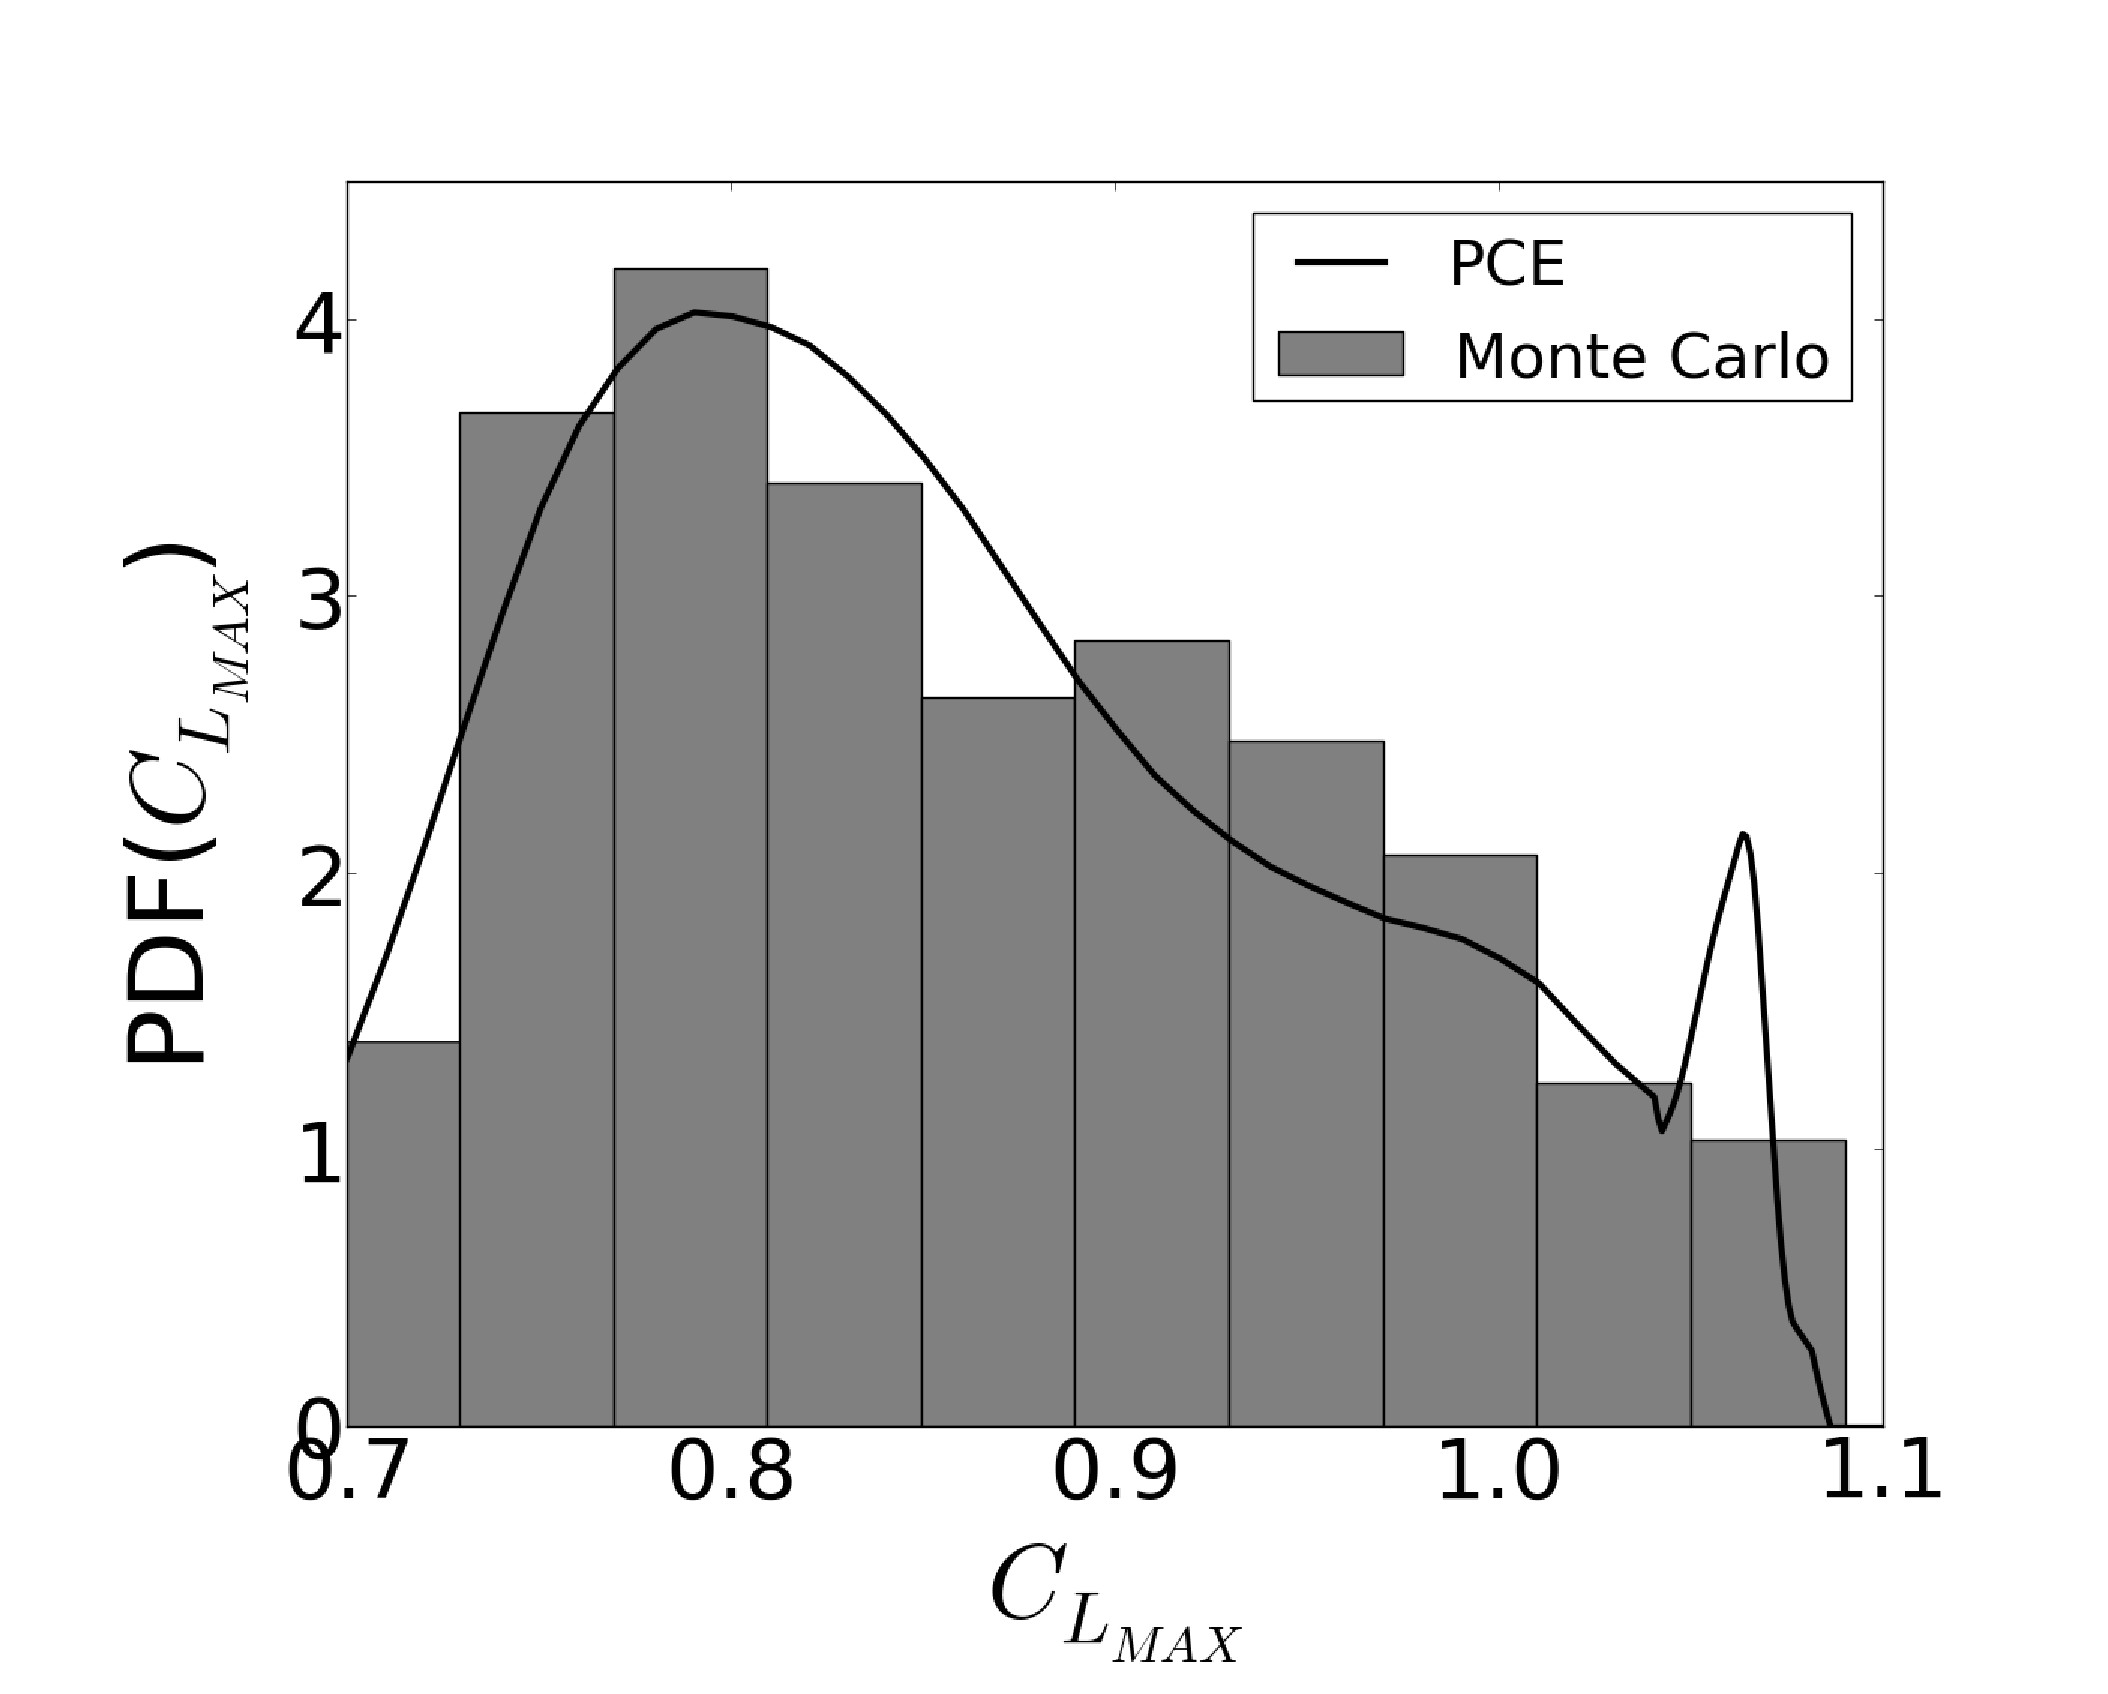
\includegraphics[width=0.65\textwidth]{MCgpcPDFMEGPCHorn_CL}
\caption{Lift Statistics}
\end{figure}
\end{minipage}
\begin{itemize}
\item Horn separation normally distributed
\item Horn height distributed as a half-Gaussian (mean = clean airfoil)
\item Performance degrades with larger horn size and separation
\end{itemize}
\end{frame}
\section{Data-Based UQ}
\label{sec-3}
\begin{frame}
\frametitle{Dataset}
\label{sec-3-1}

\vspace*{-0.0cm}\begin{figure}
      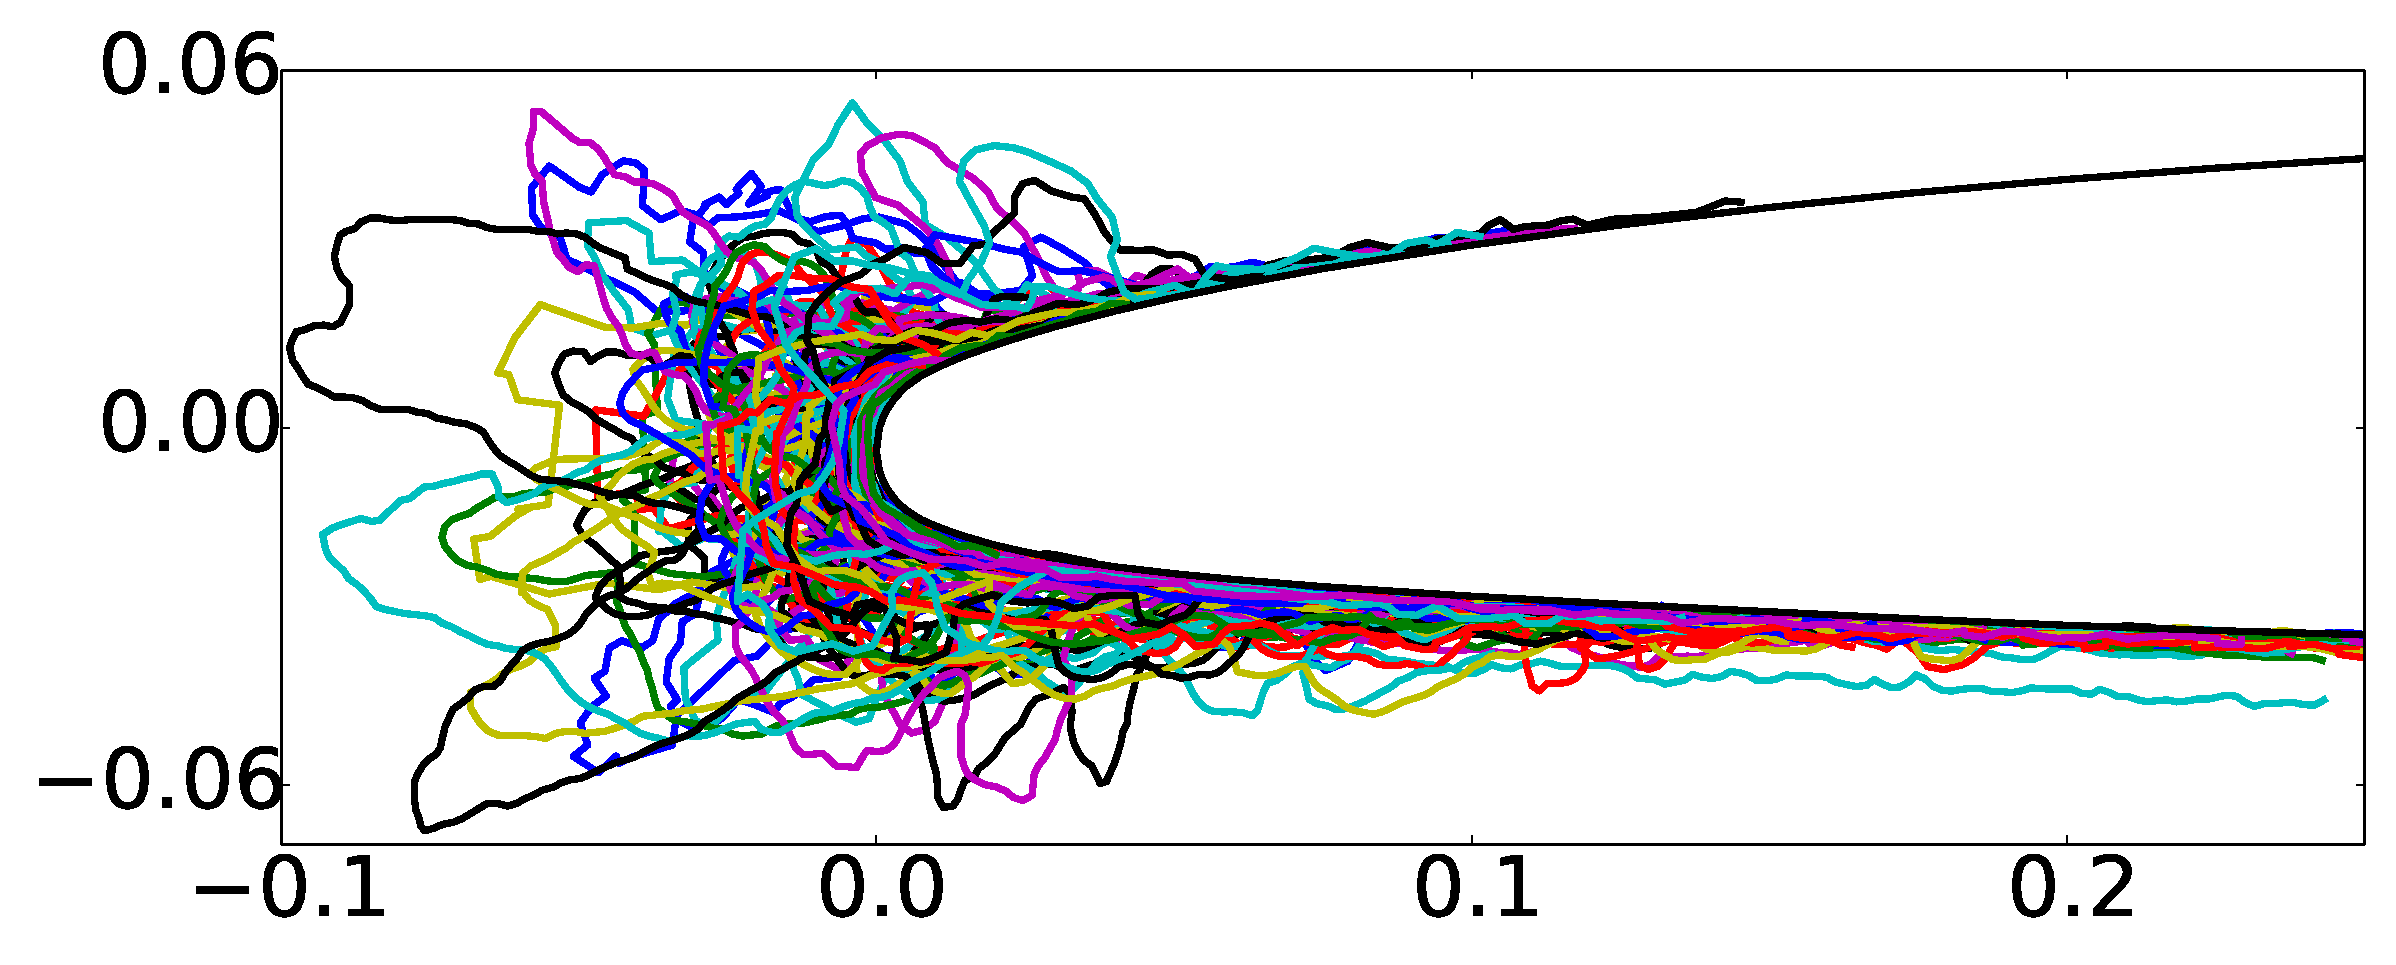
\includegraphics[width=0.5\textwidth]{GlobalDataSet}
      \caption{Wind tunnel experimental ice shapes}
\end{figure}
\begin{itemize}
\item Dataset consists of 145 experimental ice shapes
\item Obtained in icing wind tunnel at NASA Glenn\footnotemark[1]
\item Representative of a wide variety of icing conditions (temperature,
  LWC, accretion time, etc.)
\end{itemize}
  
\end{frame}
\begin{frame}
\frametitle{Data-Driven Model}
\label{sec-3-2}

\vspace*{-0.0cm}\begin{figure}
      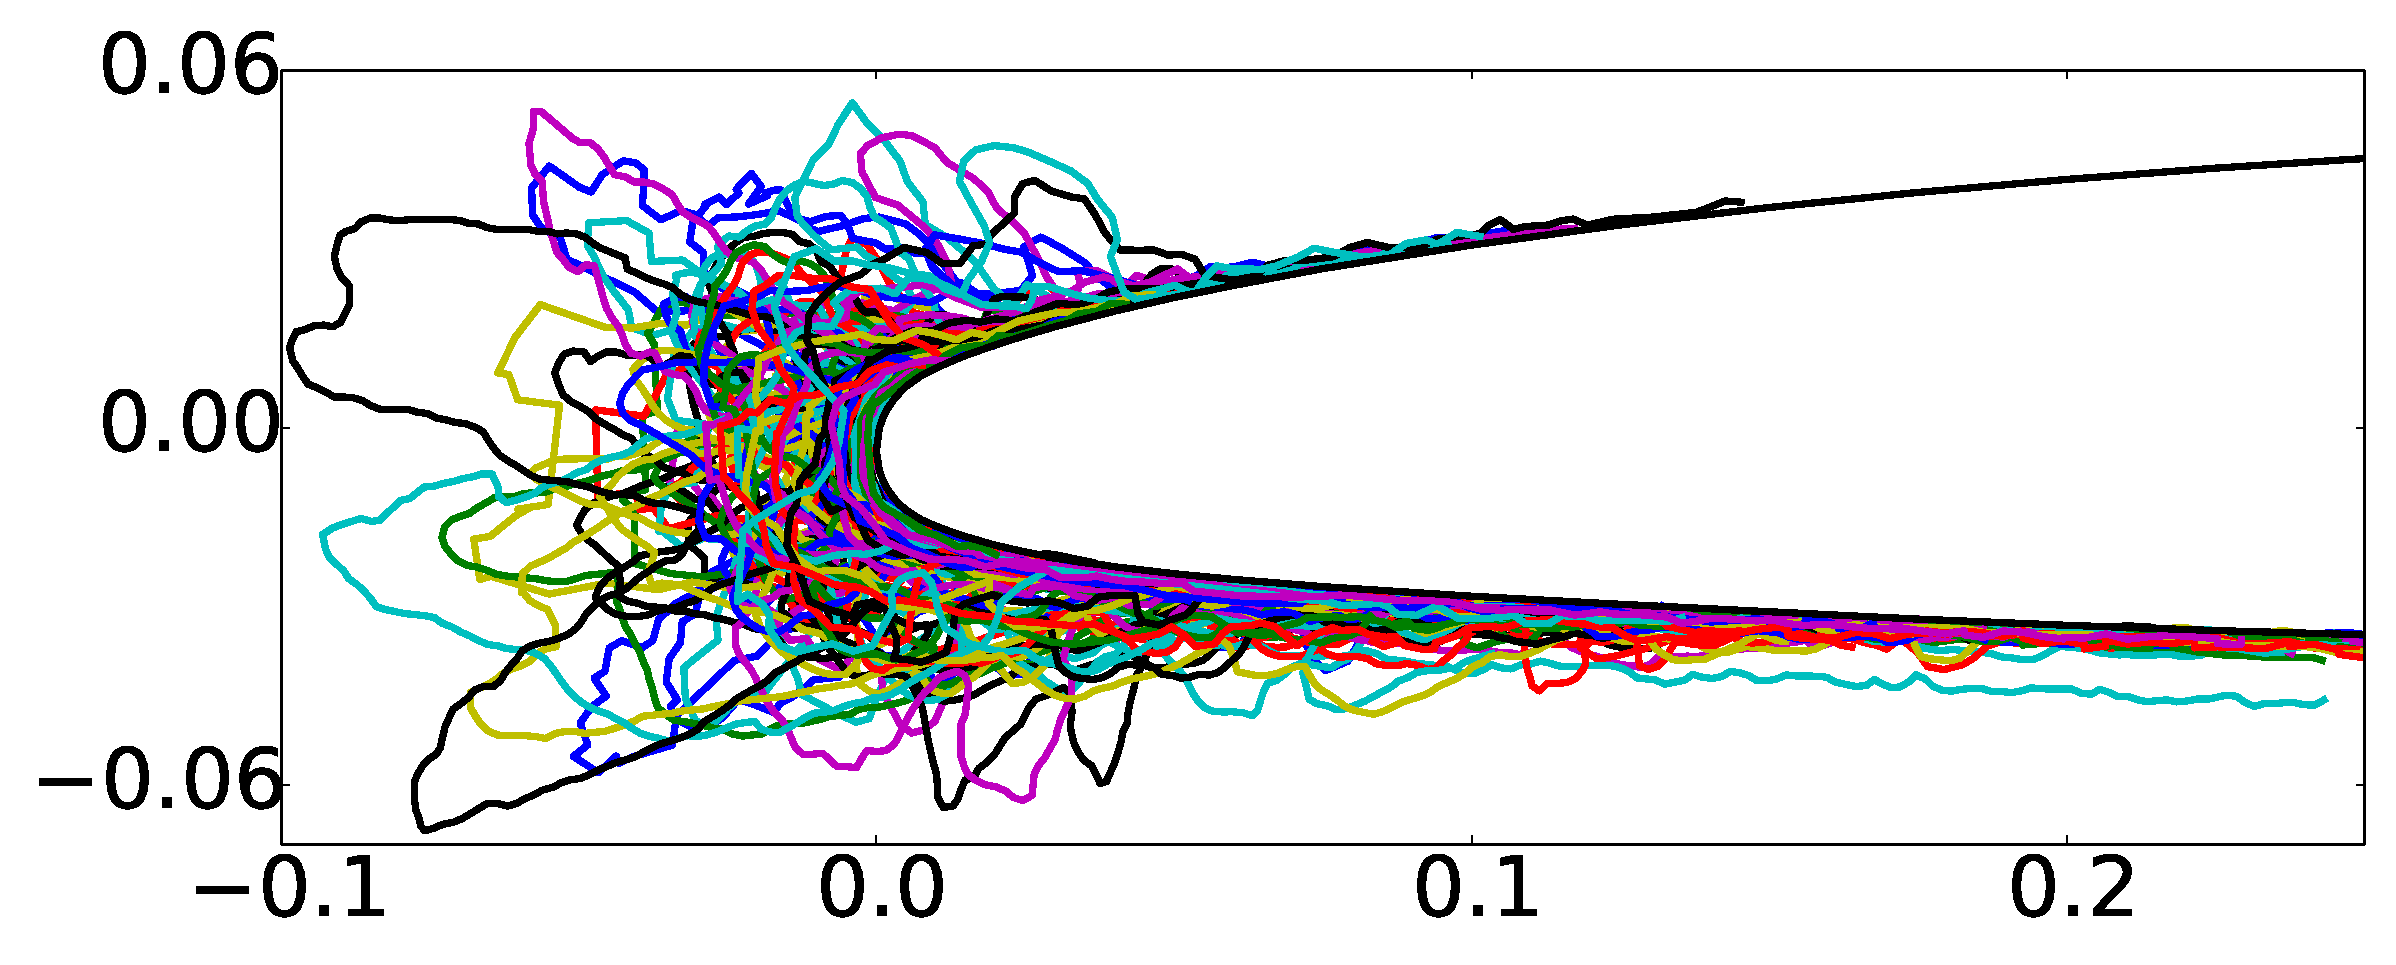
\includegraphics[width=0.5\textwidth]{GlobalDataSet}
      \caption{Wind tunnel experimental ice shapes}
\end{figure}
\textbf{Goal:} Make a purely data-driven model of icing (no equations)

\textbf{Approach:}
\begin{itemize}
\item Build low-dimensional model of shape using POD
\item Correlate POD coefficients to temperature, accretion time, LWC
\item Generate random ice shapes corresponding to given conditions
\end{itemize}
\end{frame}
\begin{frame}
\frametitle{Proper Orthogonal Decomposition (POD)}
\label{sec-3-3}

\textbf{Goal/Utility}
\begin{itemize}
\item Statistical analysis tool
\item Extracts linear, orthogonal basis that optimally explains dataset
\end{itemize}
\textbf{Method}
\begin{itemize}
\item Singular value decomposition of data matrix gives POD modes and eigenvalues
\end{itemize}
\begin{equation*}
\begin{aligned}
\mathbf{X} &=
 \begin{bmatrix}
   \vline & & \vline \\
   x_1 & \cdots & x_S \\
   \vline & & \vline \\
 \end{bmatrix}\\
 \bv{X} &= \Phi\Sigma\bv{V^*}\\
 x &\approx \sum_i^{M} c_i \phi_i
\end{aligned}
\end{equation}
\end{frame}
\begin{frame}
\frametitle{POD Eigenvalues}
\label{sec-3-4}

\vspace*{-0.0cm}\begin{figure}
      \subfigure[Magnitude.]{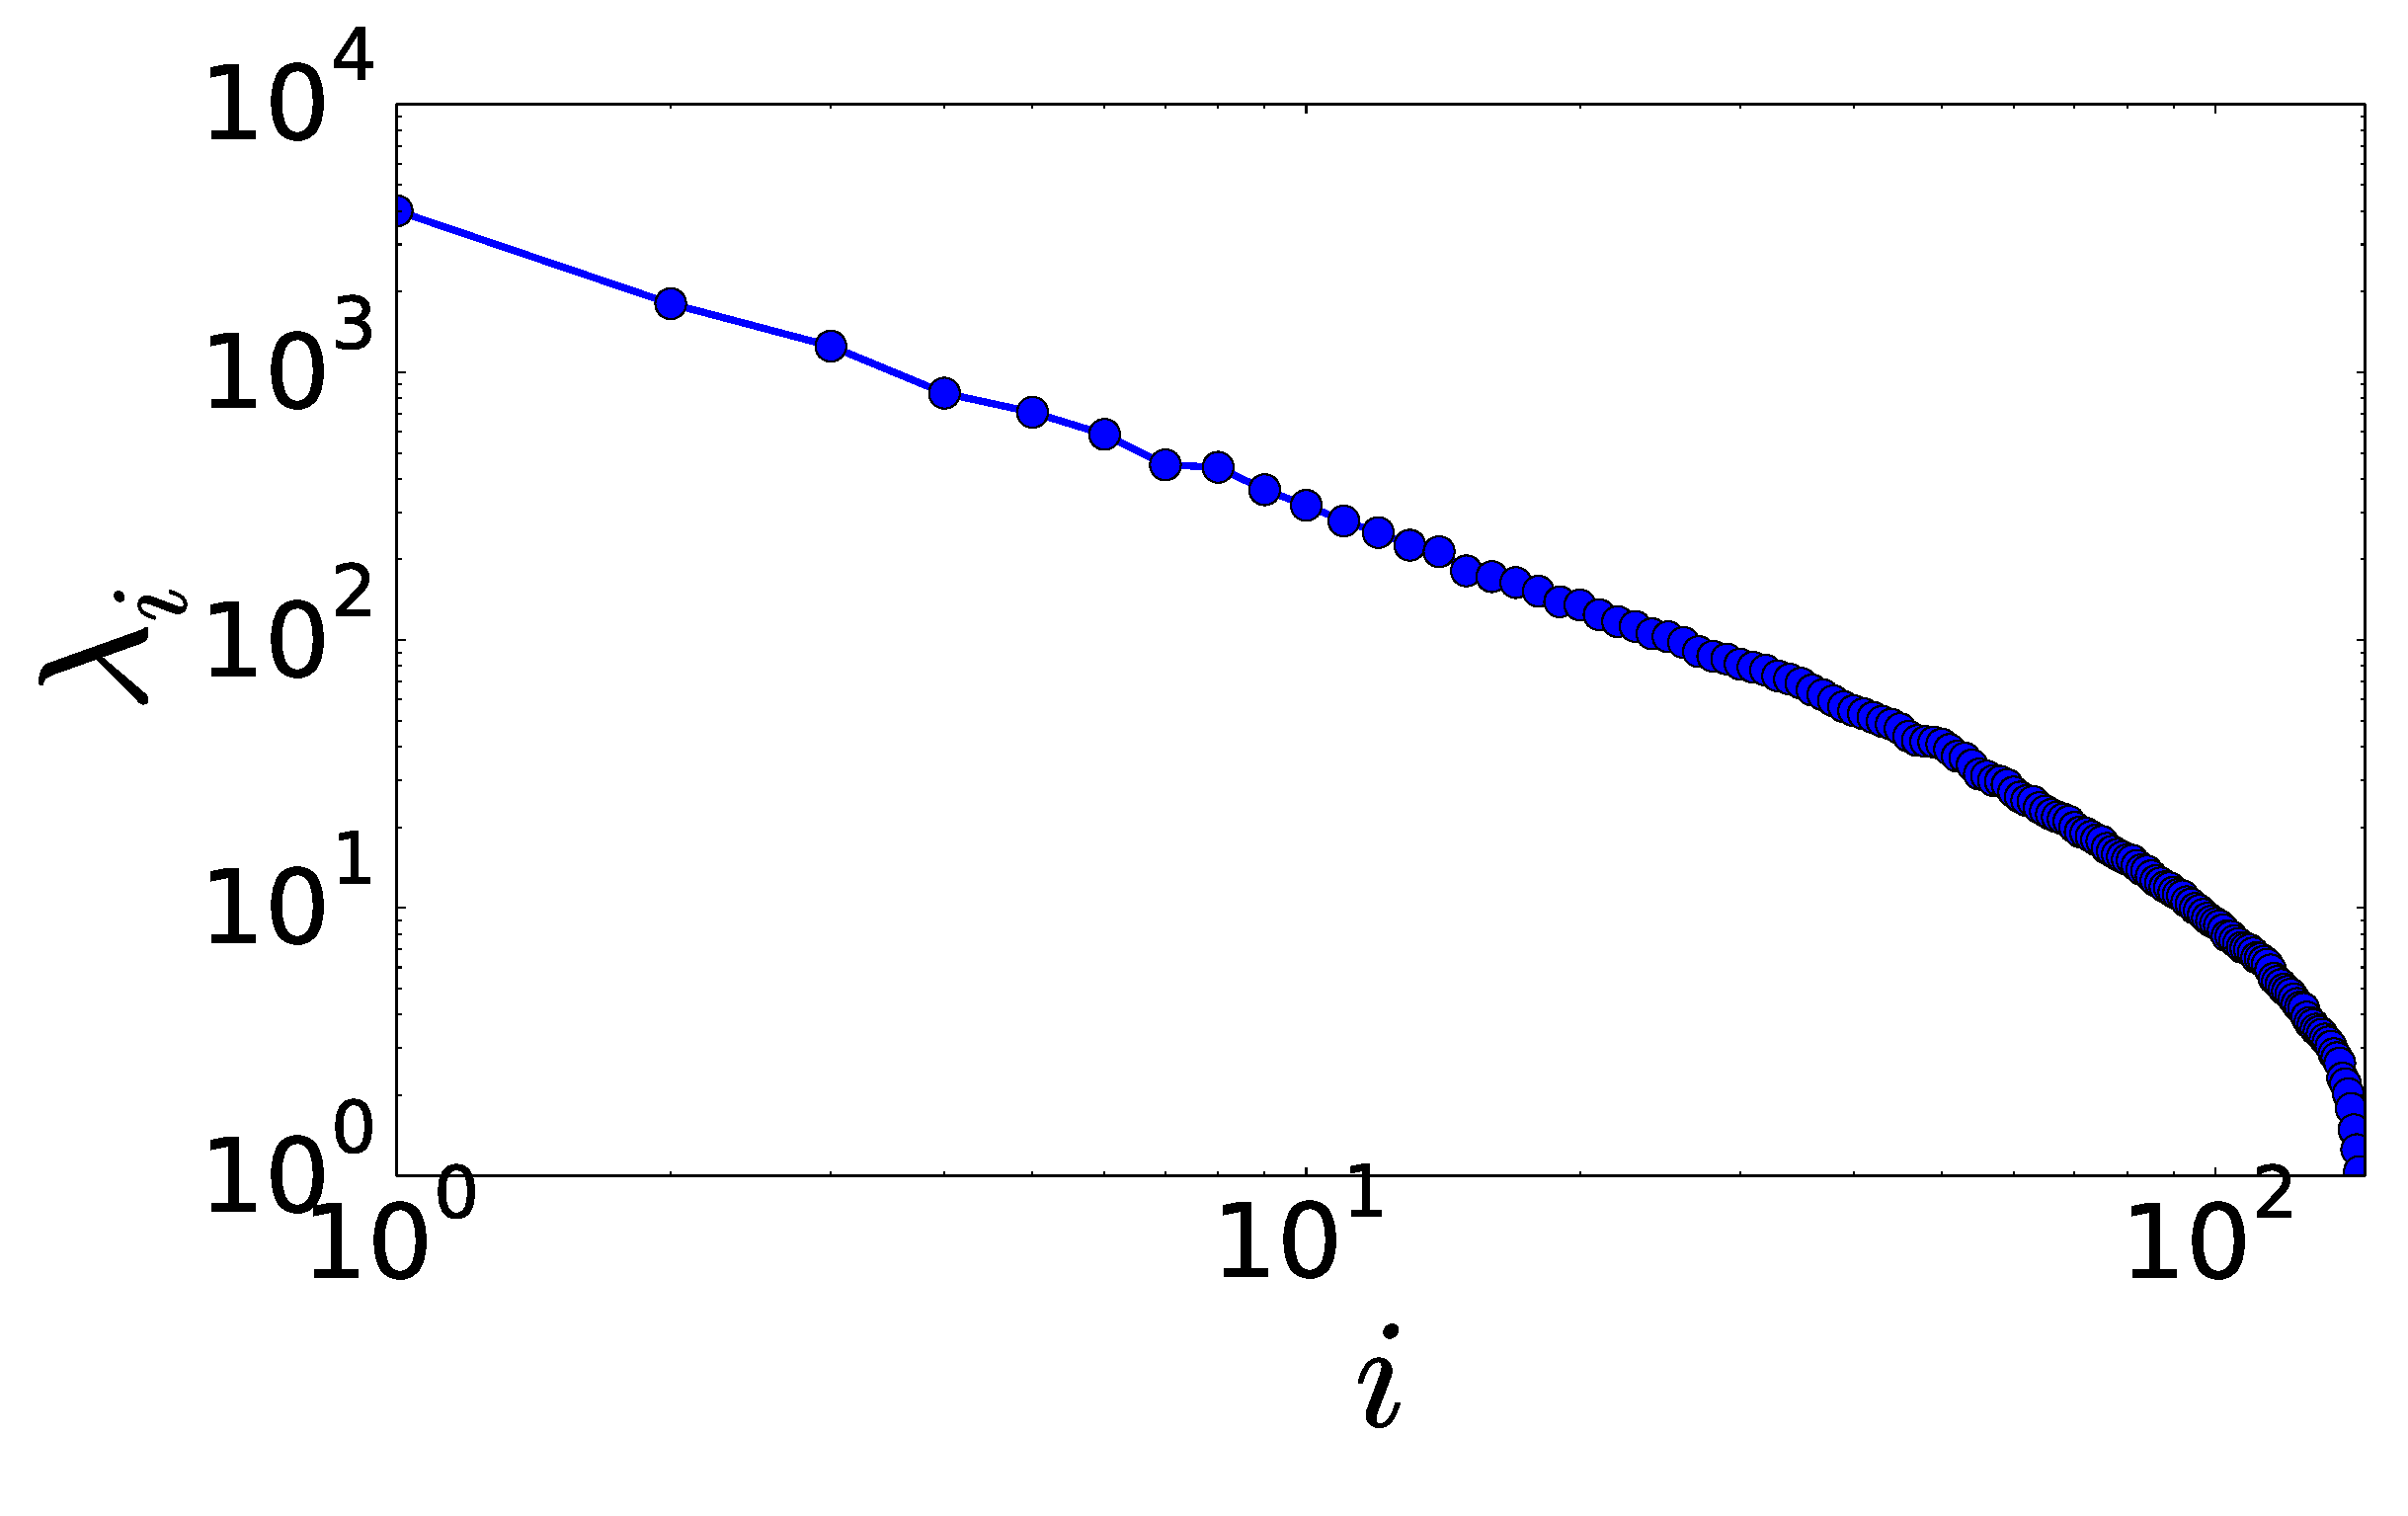
\includegraphics[width=0.4\textwidth]{PODevals.eps}}
      \subfigure[Cumulative sum.]{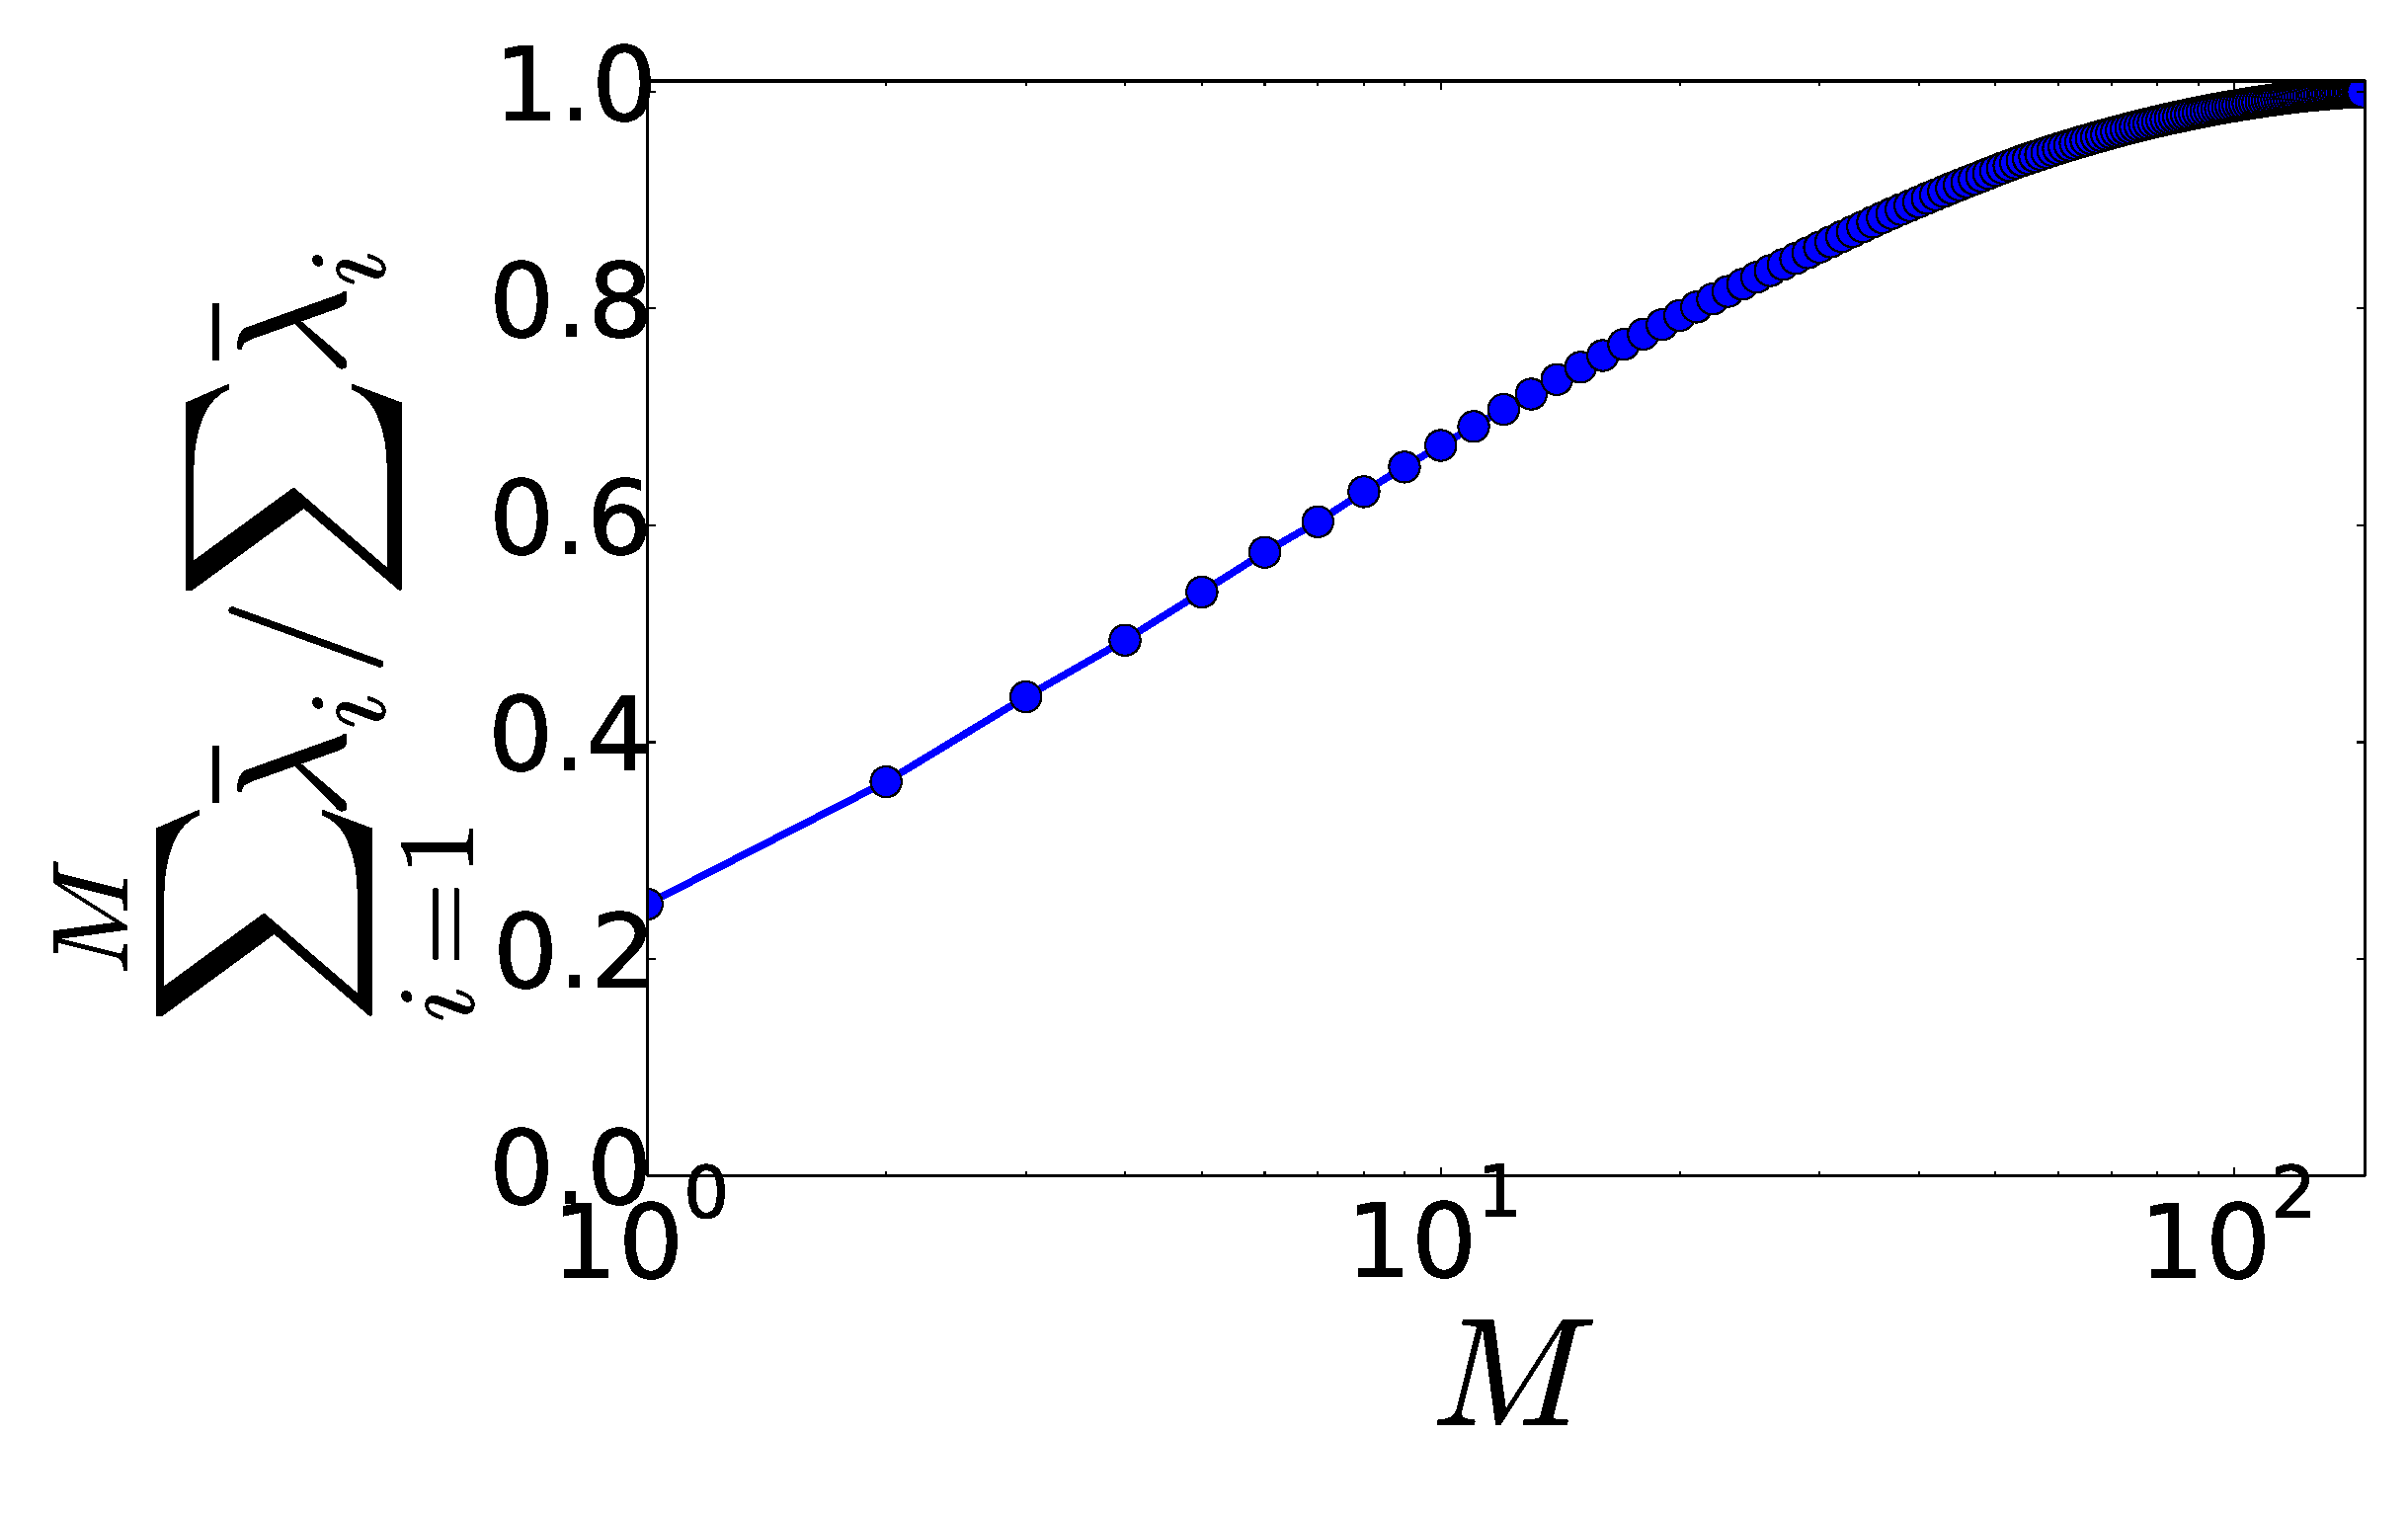
\includegraphics[width=0.4\textwidth]{CumsumPODevals.eps}}
      \caption{POD eigenvalues.}
\end{figure}

\begin{itemize}
\item 2/3 of cumulative sum contained in first 10 modes
\item 2/3 of statistical variation contained in first 10 modes
\item Truncate model at 10 modes
\end{itemize}
\end{frame}
\begin{frame}
\frametitle{POD Modes}
\label{sec-3-5}

\vspace*{0.75cm}\begin{figure}
      \vspace*{-1.75cm}\subfigure{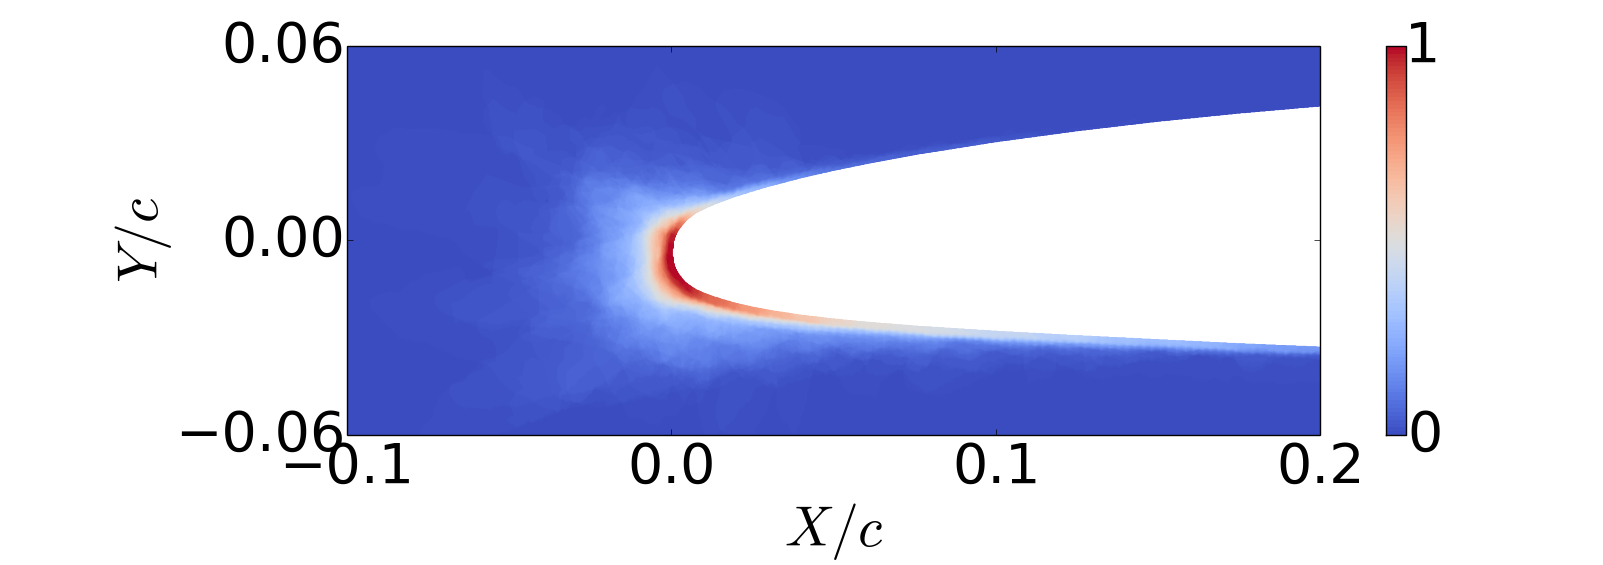
\includegraphics[width=0.4\textwidth]{MEAN}} \\
      \vspace*{-0.75cm}\subfigure{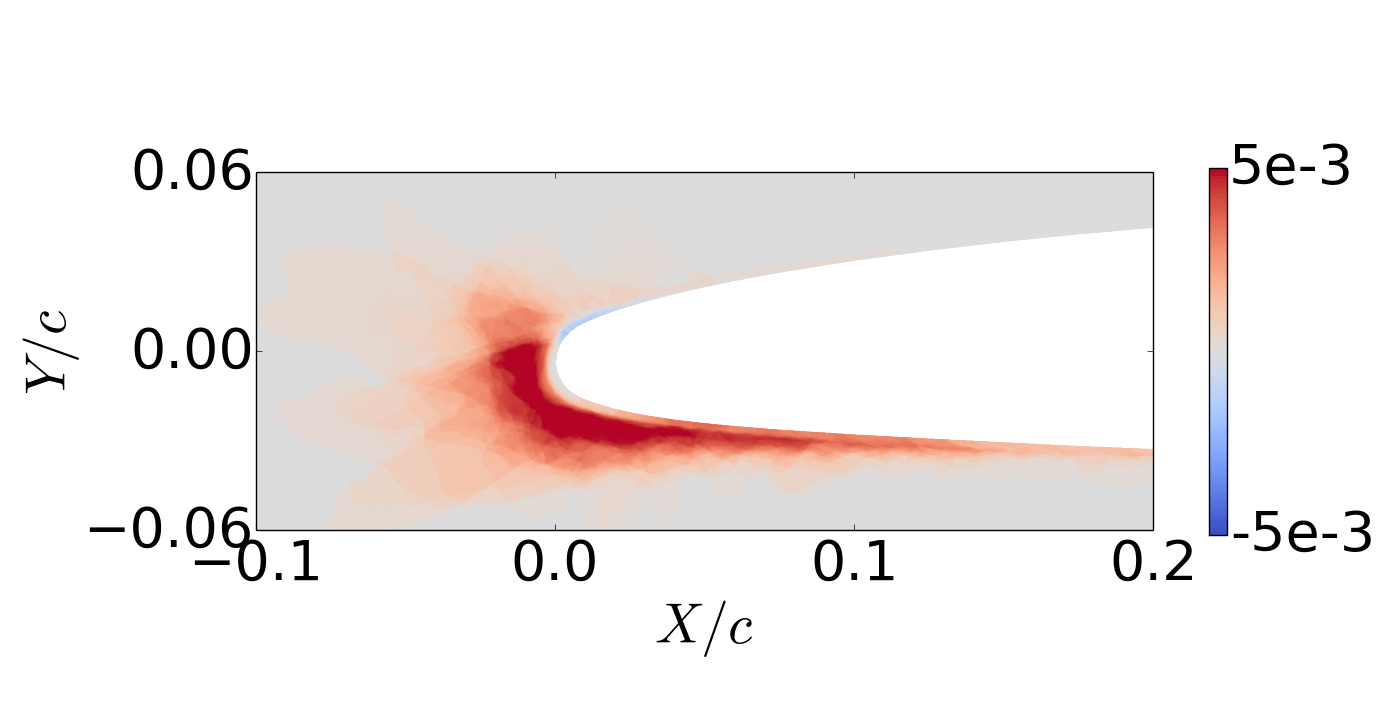
\includegraphics[width=0.4\textwidth]{MODE1}}
      \vspace*{-0.75cm}\subfigure{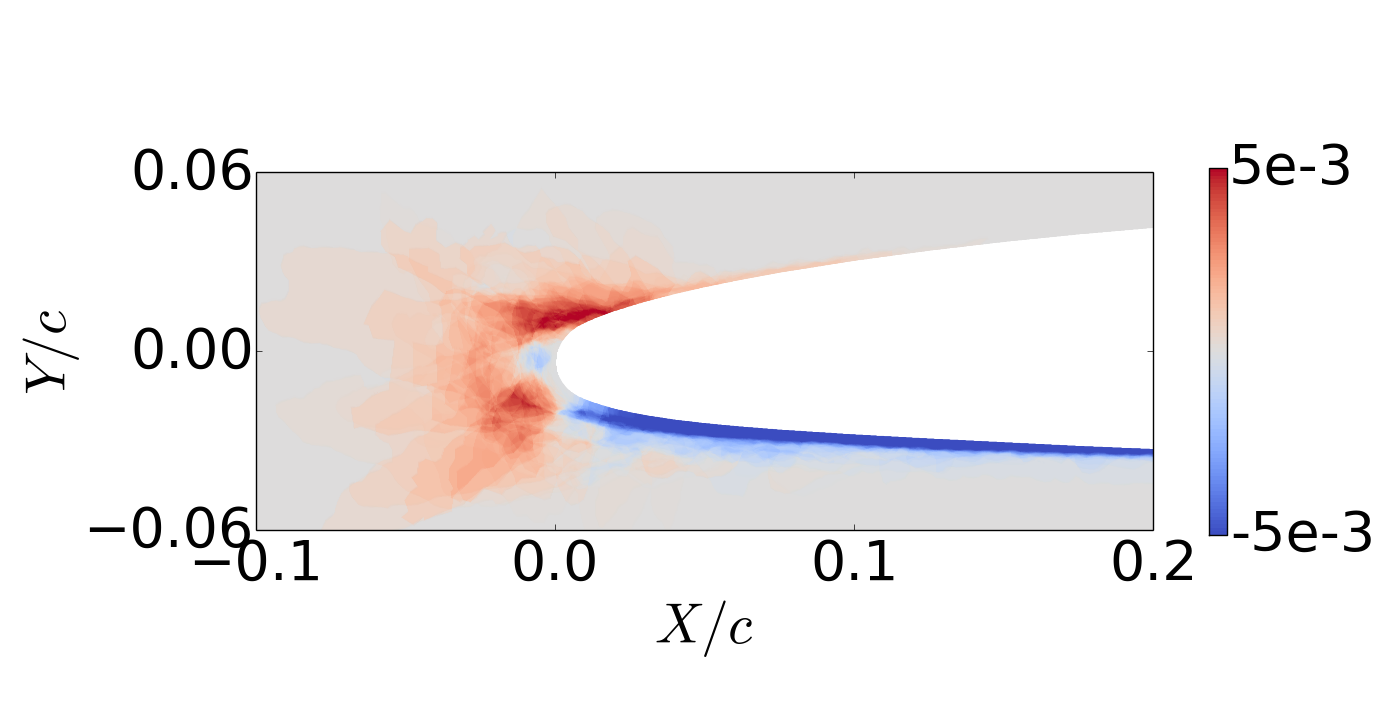
\includegraphics[width=0.4\textwidth]{MODE2}}
      \vspace*{-0.75cm}\subfigure{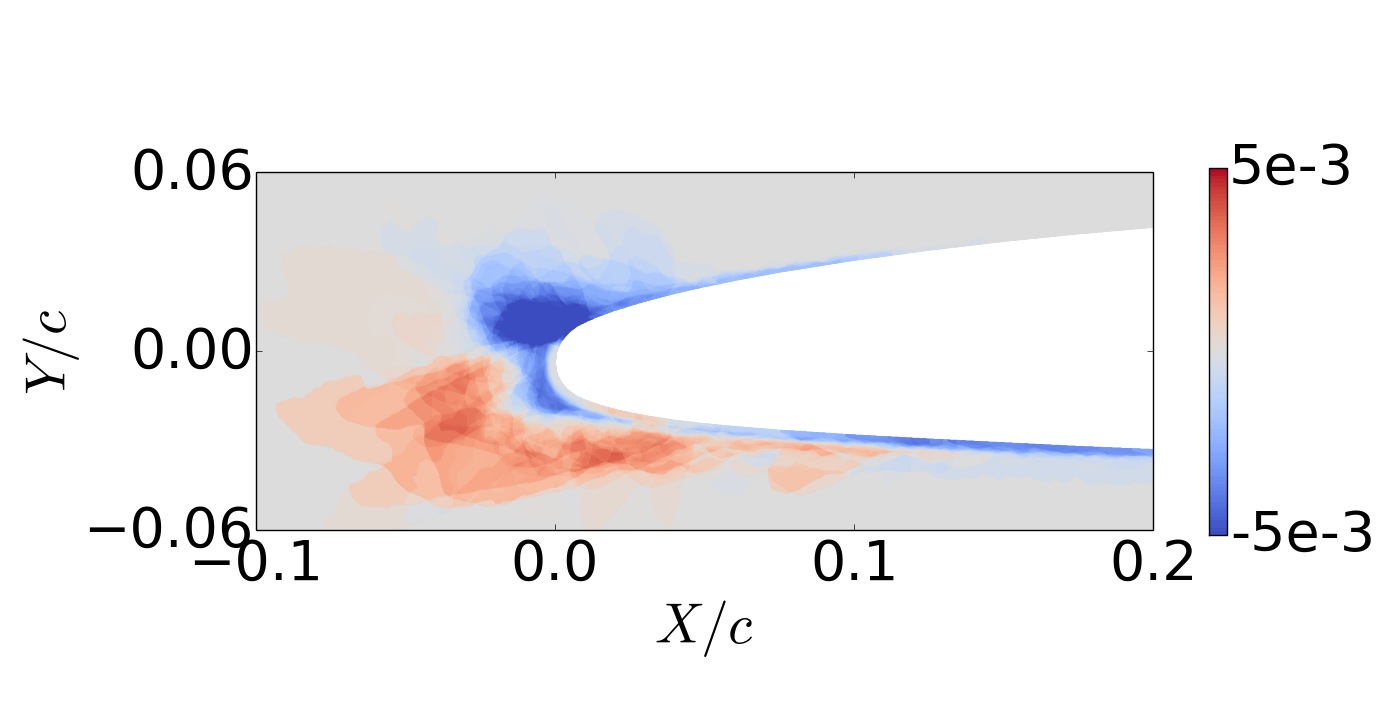
\includegraphics[width=0.4\textwidth]{MODE3}}
      \vspace*{-0.75cm}\subfigure{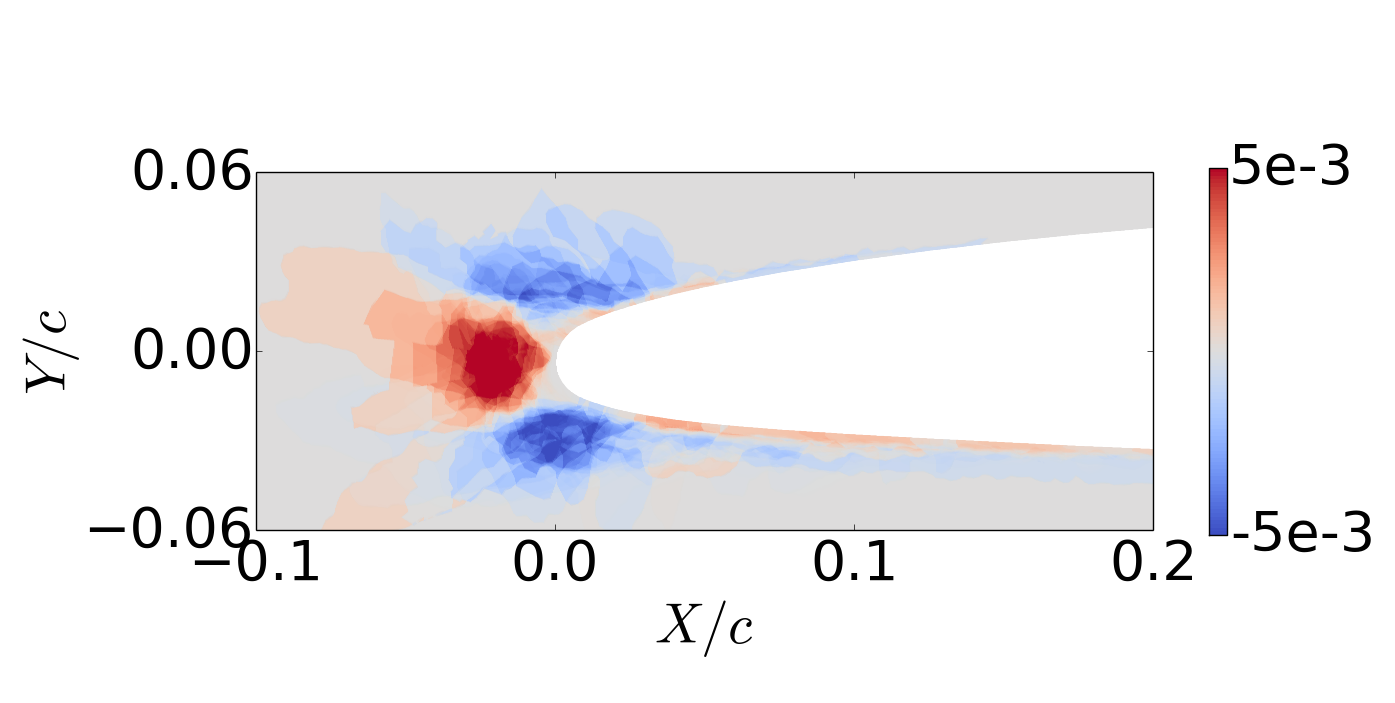
\includegraphics[width=0.4\textwidth]{MODE4}}
      \vspace*{1cm}\caption{Mean and POD modes.}
\end{figure}

\begin{itemize}
\item Represent ice shapes as composite sum of these pictures
\item Modes 1 and 2 simply add ice mass
\item Modes 3 and 4 switch between upper/lower surface horns and rime
\item Higher order modes contain more extreme shape perturbations
\end{itemize}
\end{frame}
\begin{frame}
\frametitle{POD Reconstructions}
\label{sec-3-6}

\begin{figure}
      \vspace*{-0.5cm}\subfigure{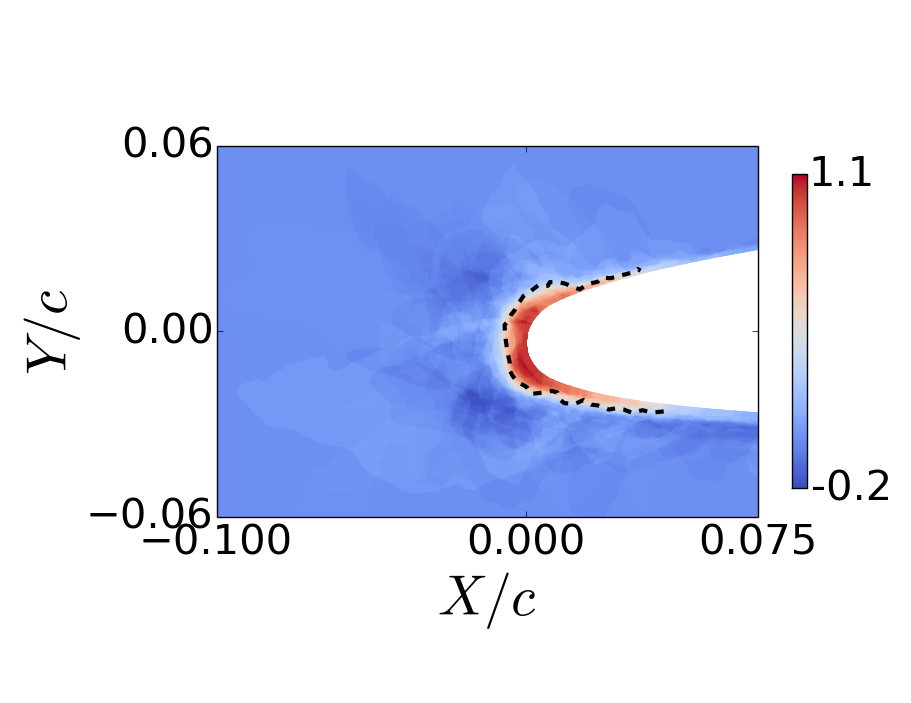
\includegraphics[width=0.3\textwidth]{UnfilteredReconstructionEx2.png}}
      \vspace*{-0.5cm}\subfigure{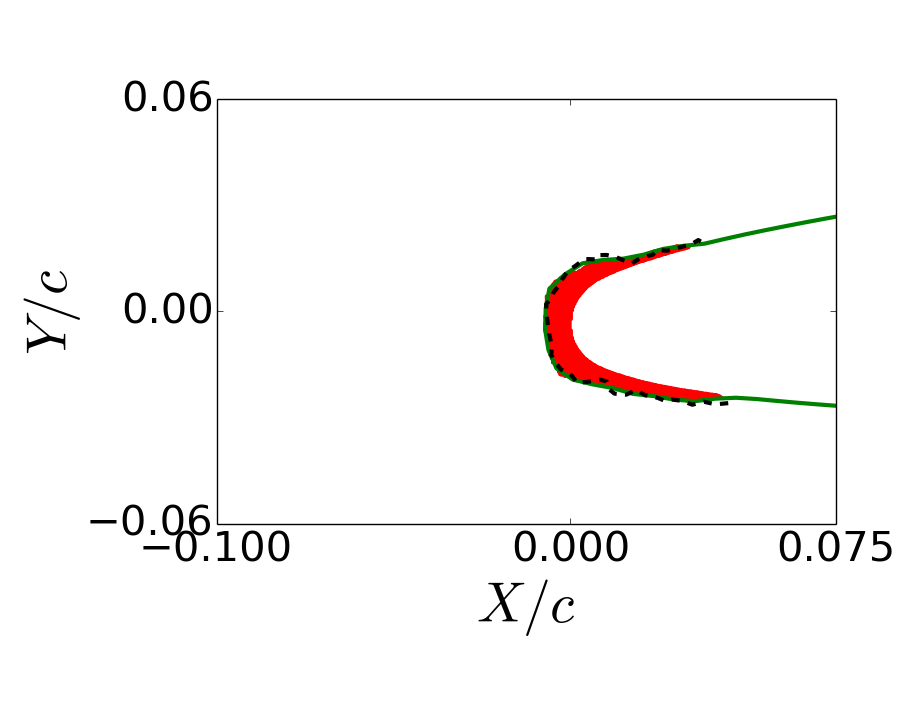
\includegraphics[width=0.3\textwidth]{FilteredReconstructionEx2.png}} \\
      \vspace*{-0.5cm}\subfigure{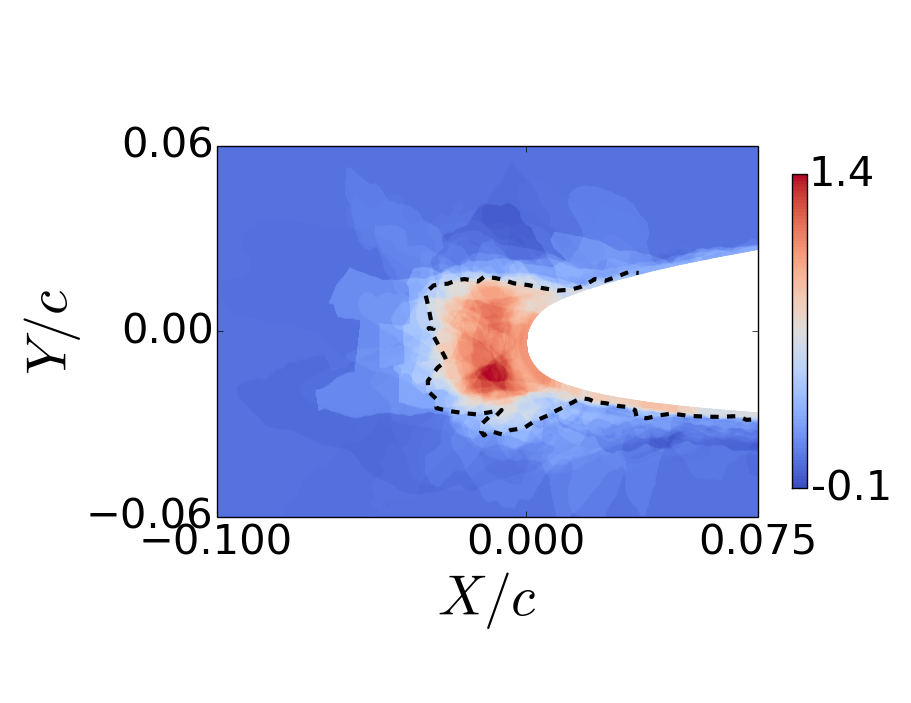
\includegraphics[width=0.3\textwidth]{UnfilteredReconstructionEx3.png}}
      \vspace*{-0.5cm}\subfigure{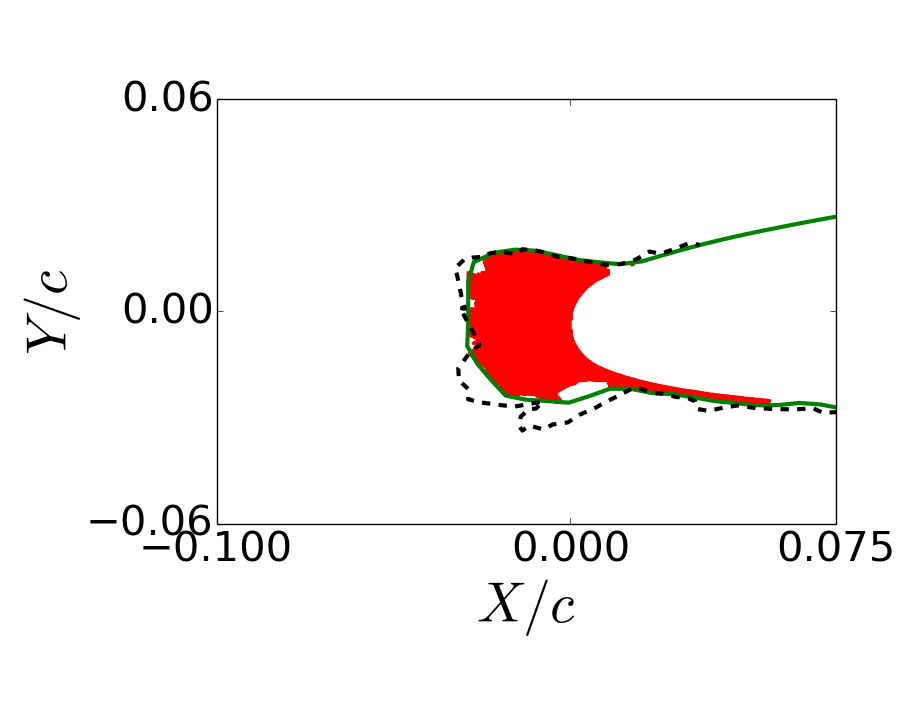
\includegraphics[width=0.3\textwidth]{FilteredReconstructionEx3.png}} \\
      \vspace*{-0.5cm}\subfigure{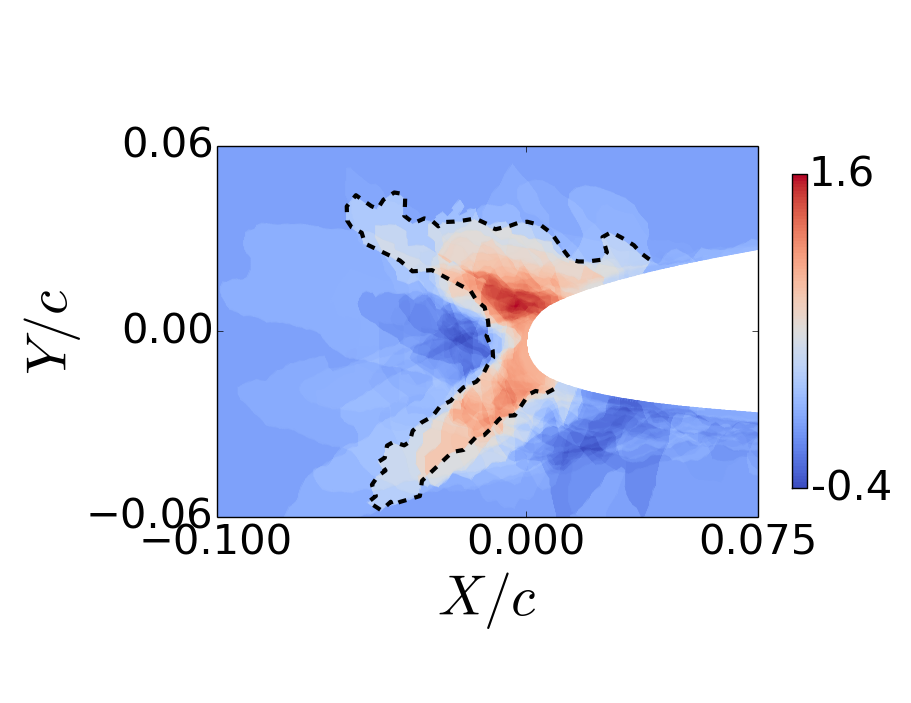
\includegraphics[width=0.3\textwidth]{UnfilteredReconstructionEx1.png}}
      \vspace*{-0.5cm}\subfigure{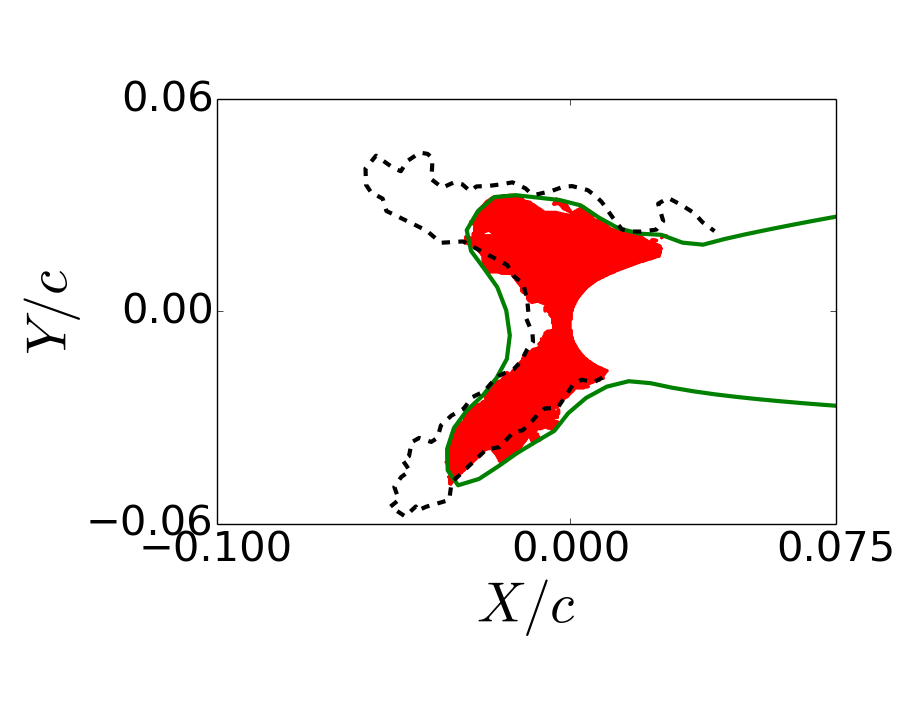
\includegraphics[width=0.3\textwidth]{FilteredReconstructionEx1.png}}
      \vspace*{0cm}\caption{POD reconstructions.}
\end{figure}

\begin{itemize}
\item Agreement is great for shapes close to mean, less good for extreme shapes
\end{itemize}
\end{frame}
\begin{frame}
\frametitle{Link Physical Conditions to Modes}
\label{sec-3-7}

\vspace*{-0.5cm}\begin{figure}
      \vspace*{-0.4cm}\subfigure{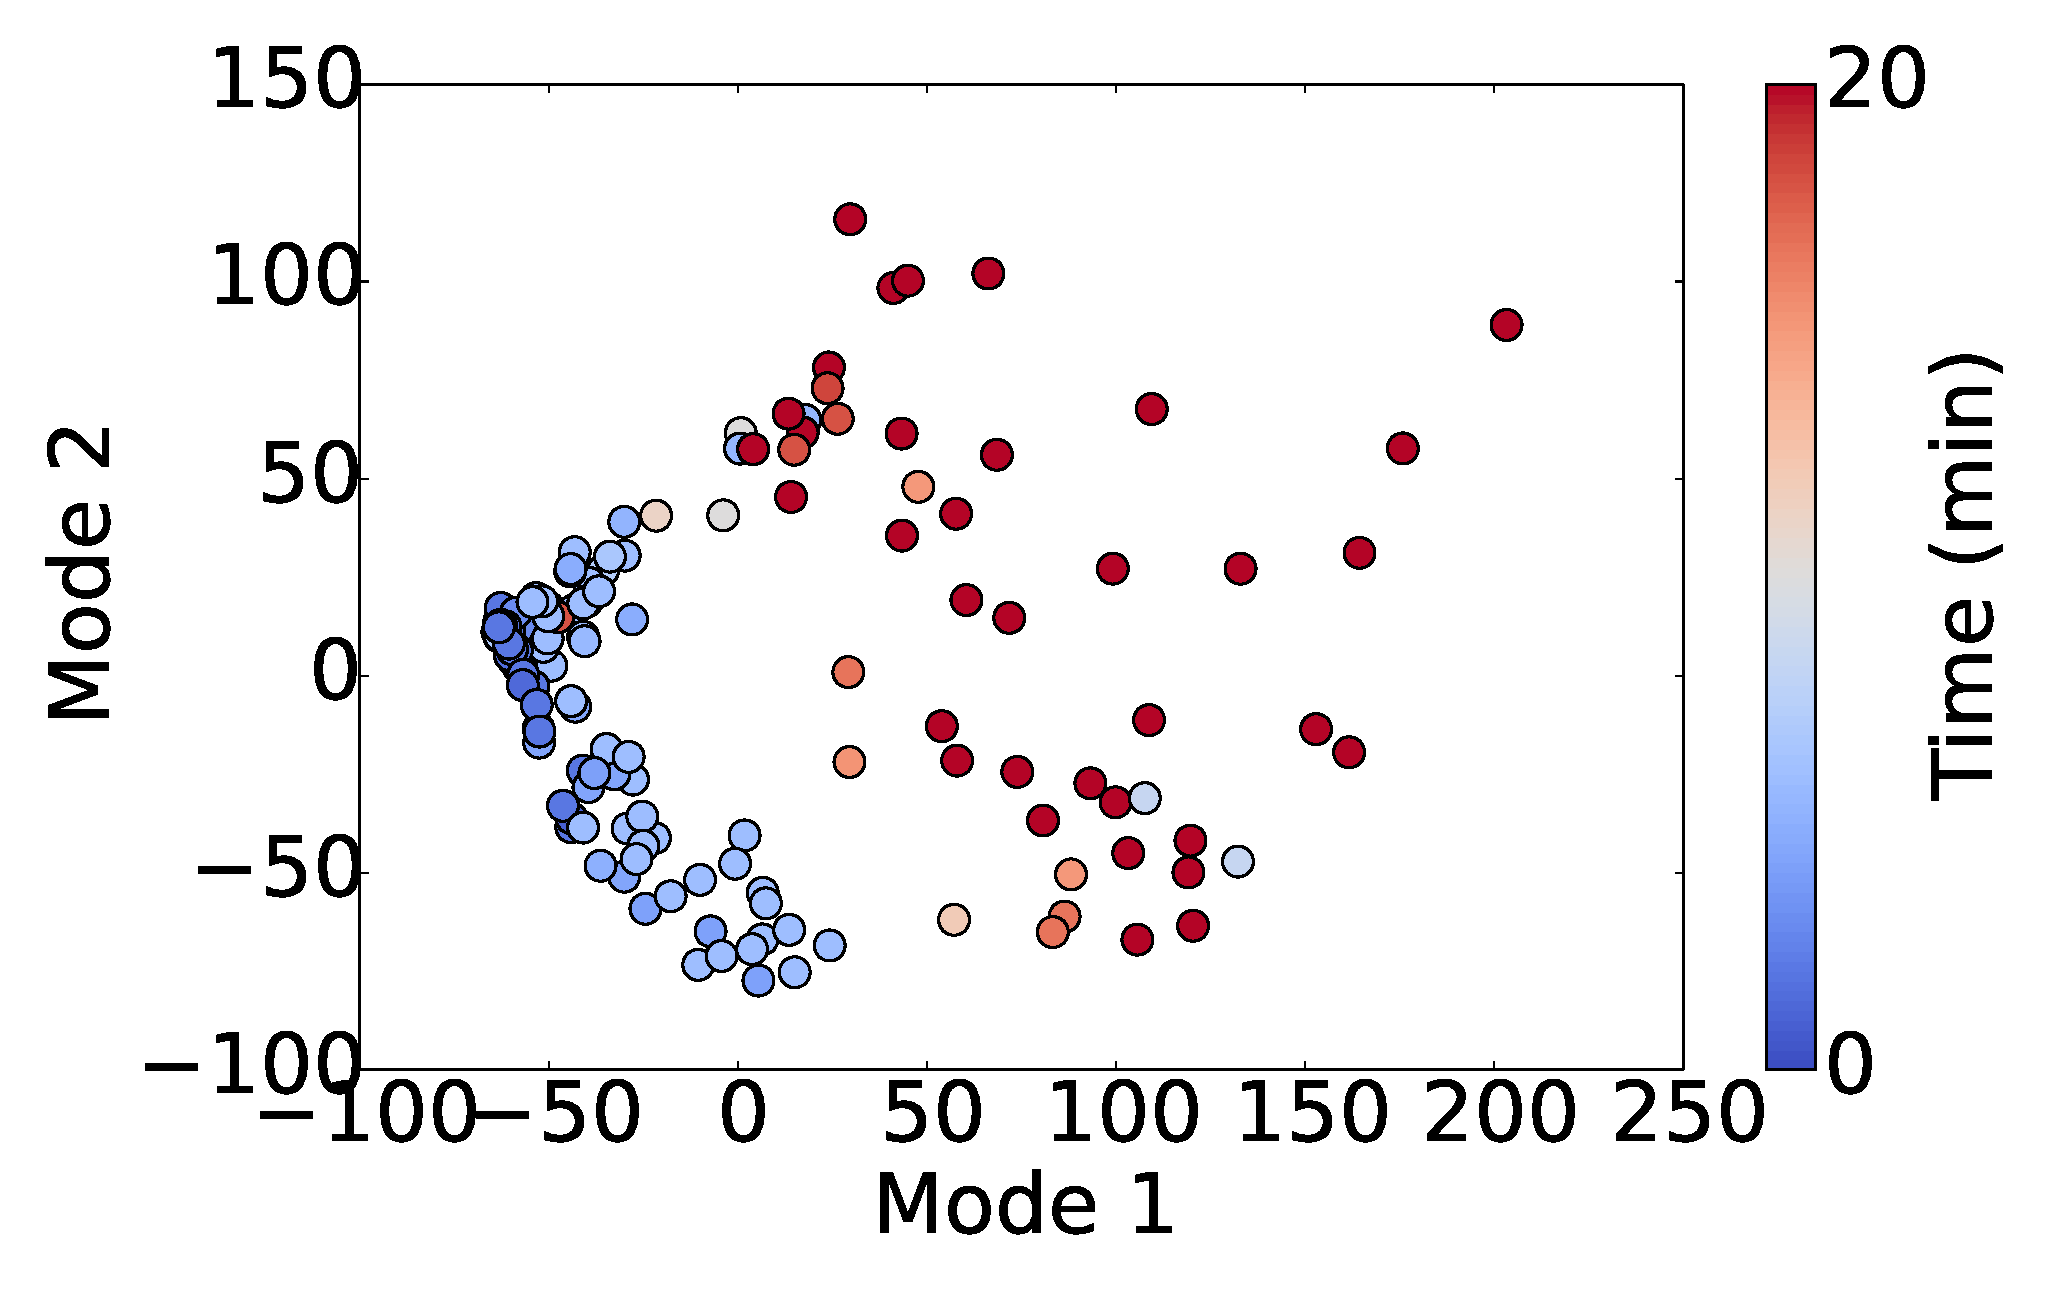
\includegraphics[width=0.35\textwidth]{10ParamMode1Mode2Time}}
      \vspace*{-0.4cm}\subfigure{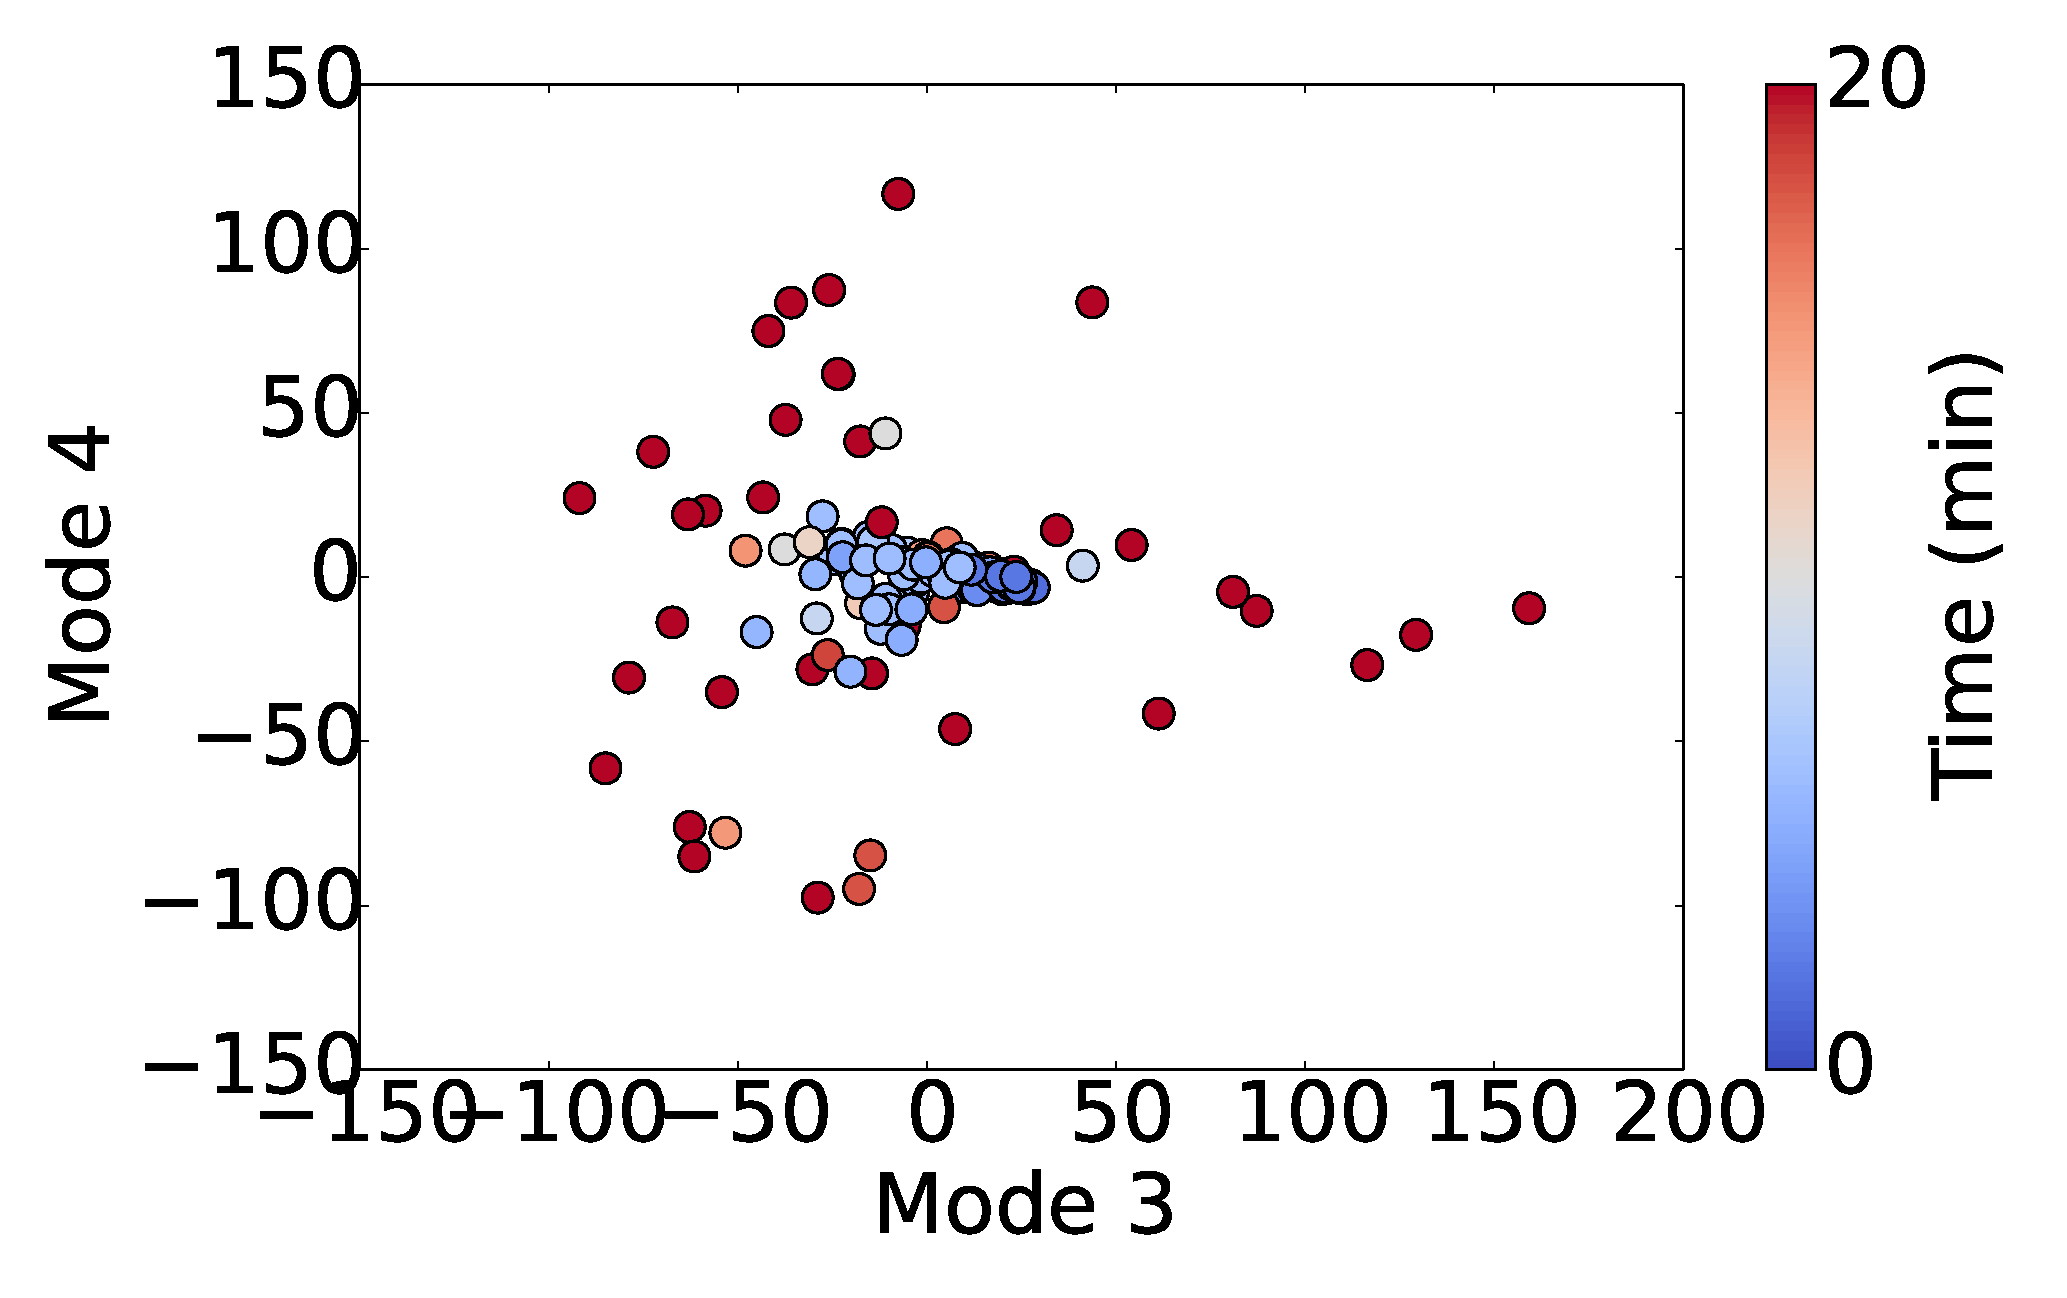
\includegraphics[width=0.35\textwidth]{10ParamMode3Mode4Time}} \\
      \vspace*{-0.35cm}\subfigure{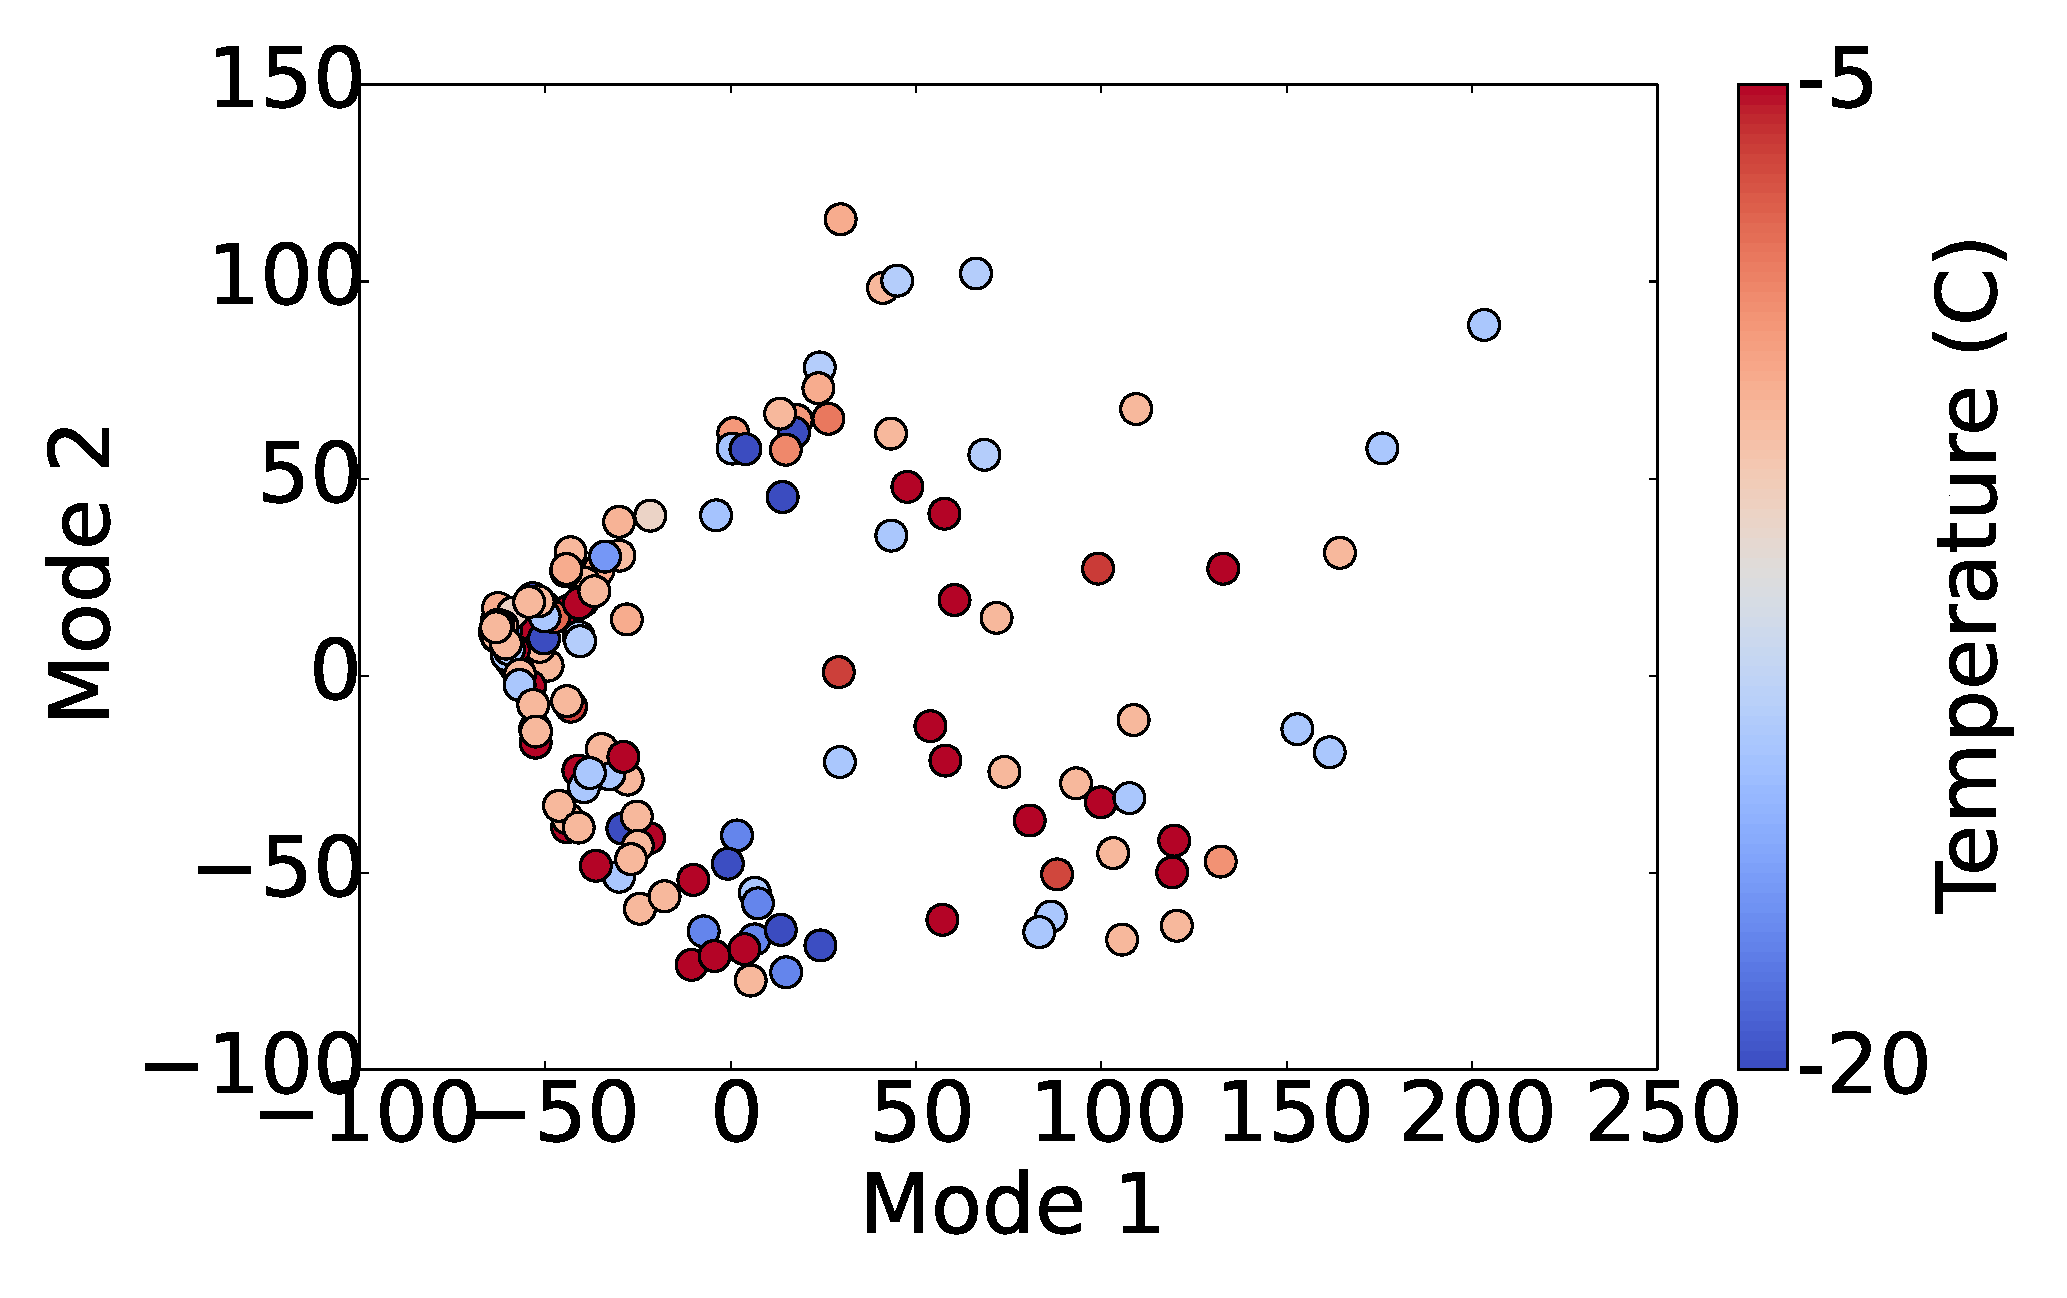
\includegraphics[width=0.35\textwidth]{10ParamMode1Mode2Temp}}
      \vspace*{-0.35cm}\subfigure{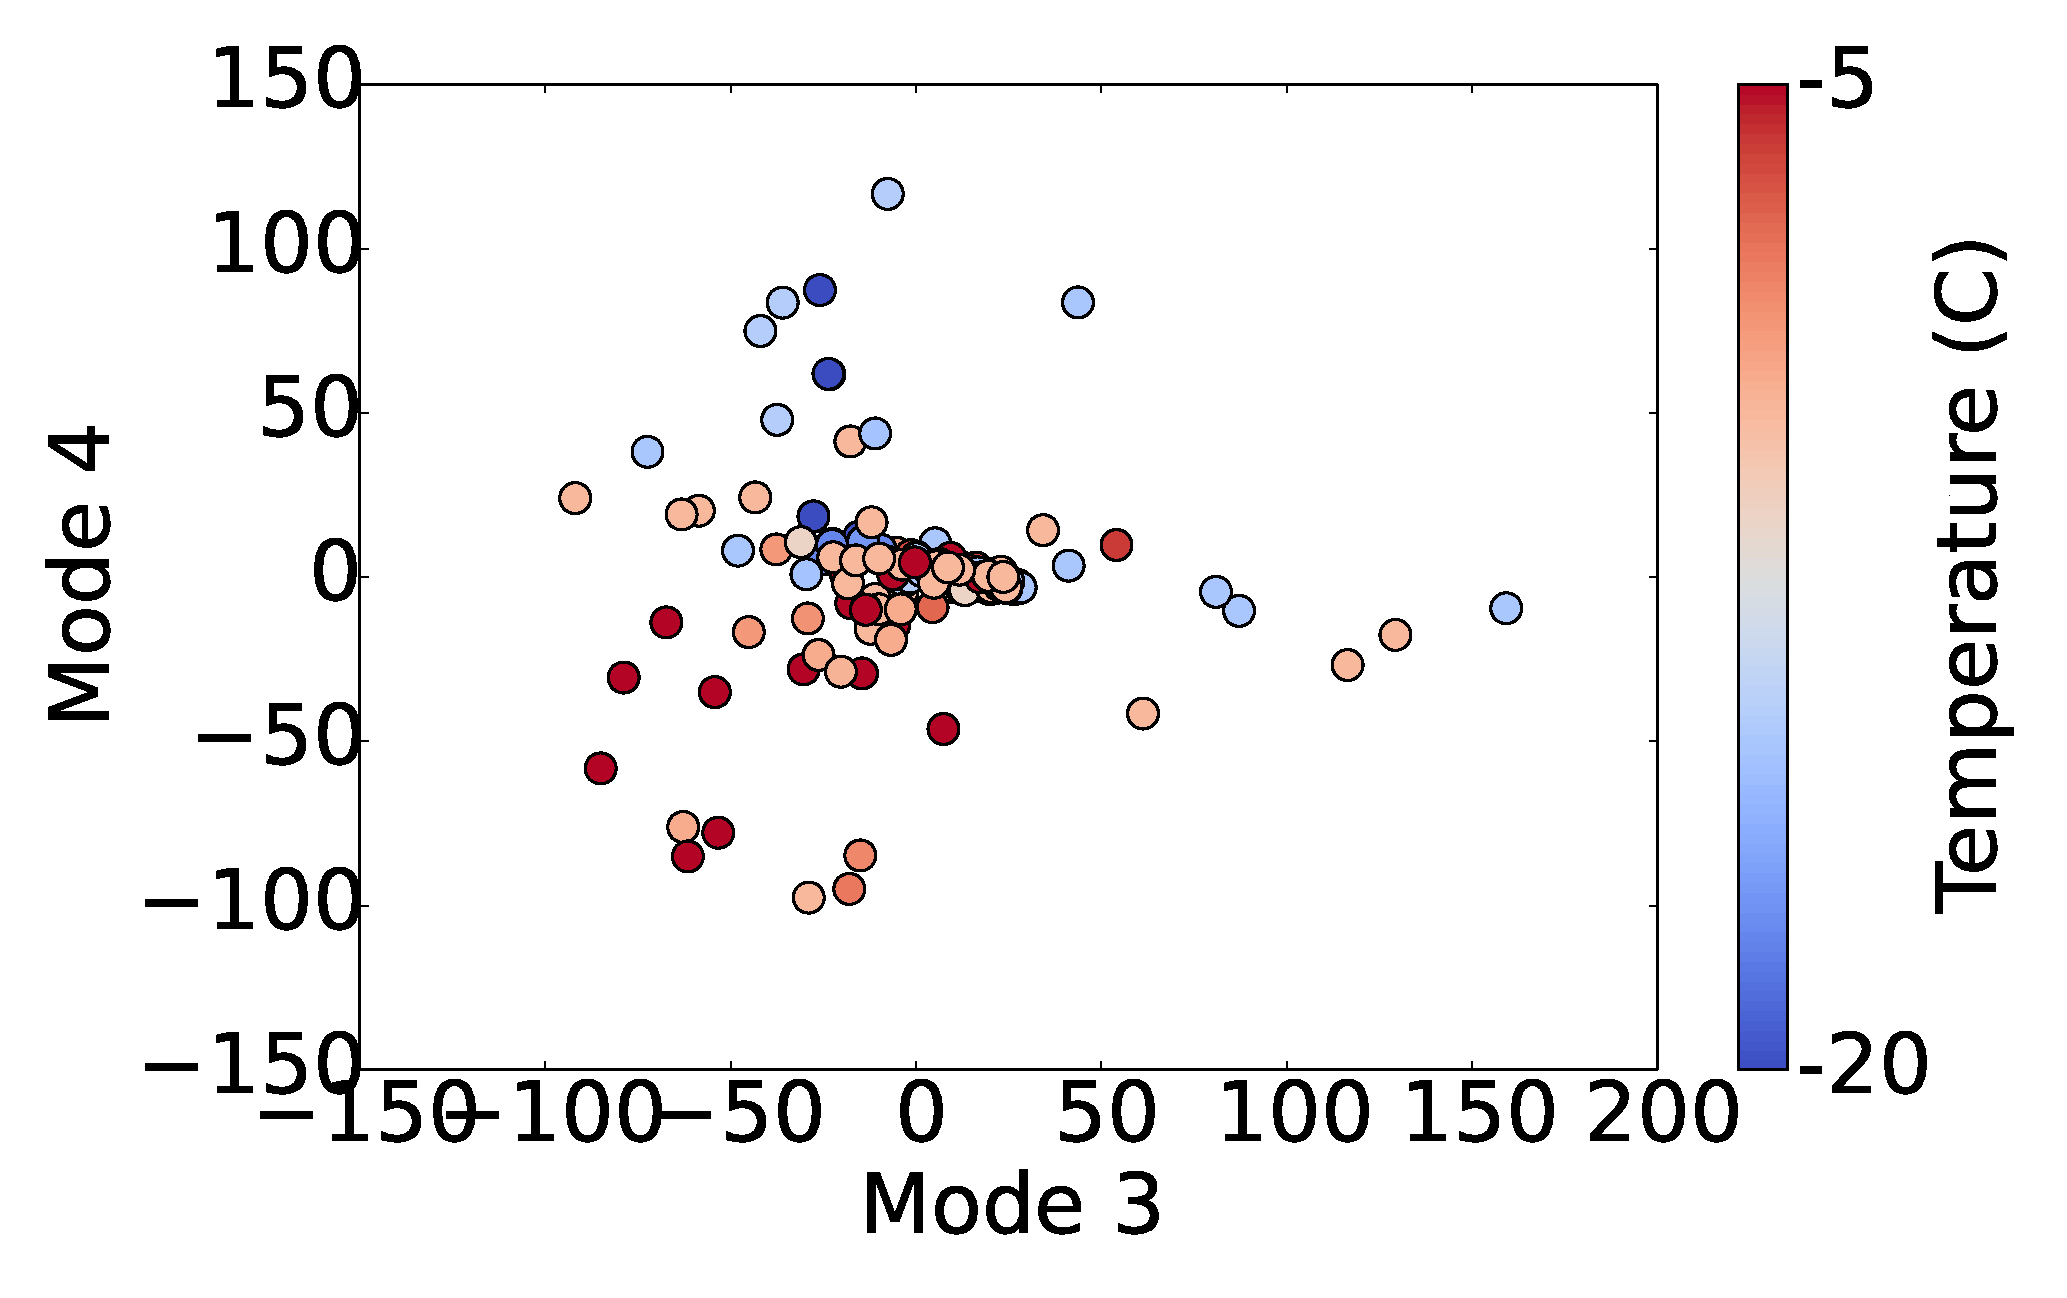
\includegraphics[width=0.35\textwidth]{10ParamMode3Mode4Temp}} \\
      \vspace*{-0.35cm}\subfigure{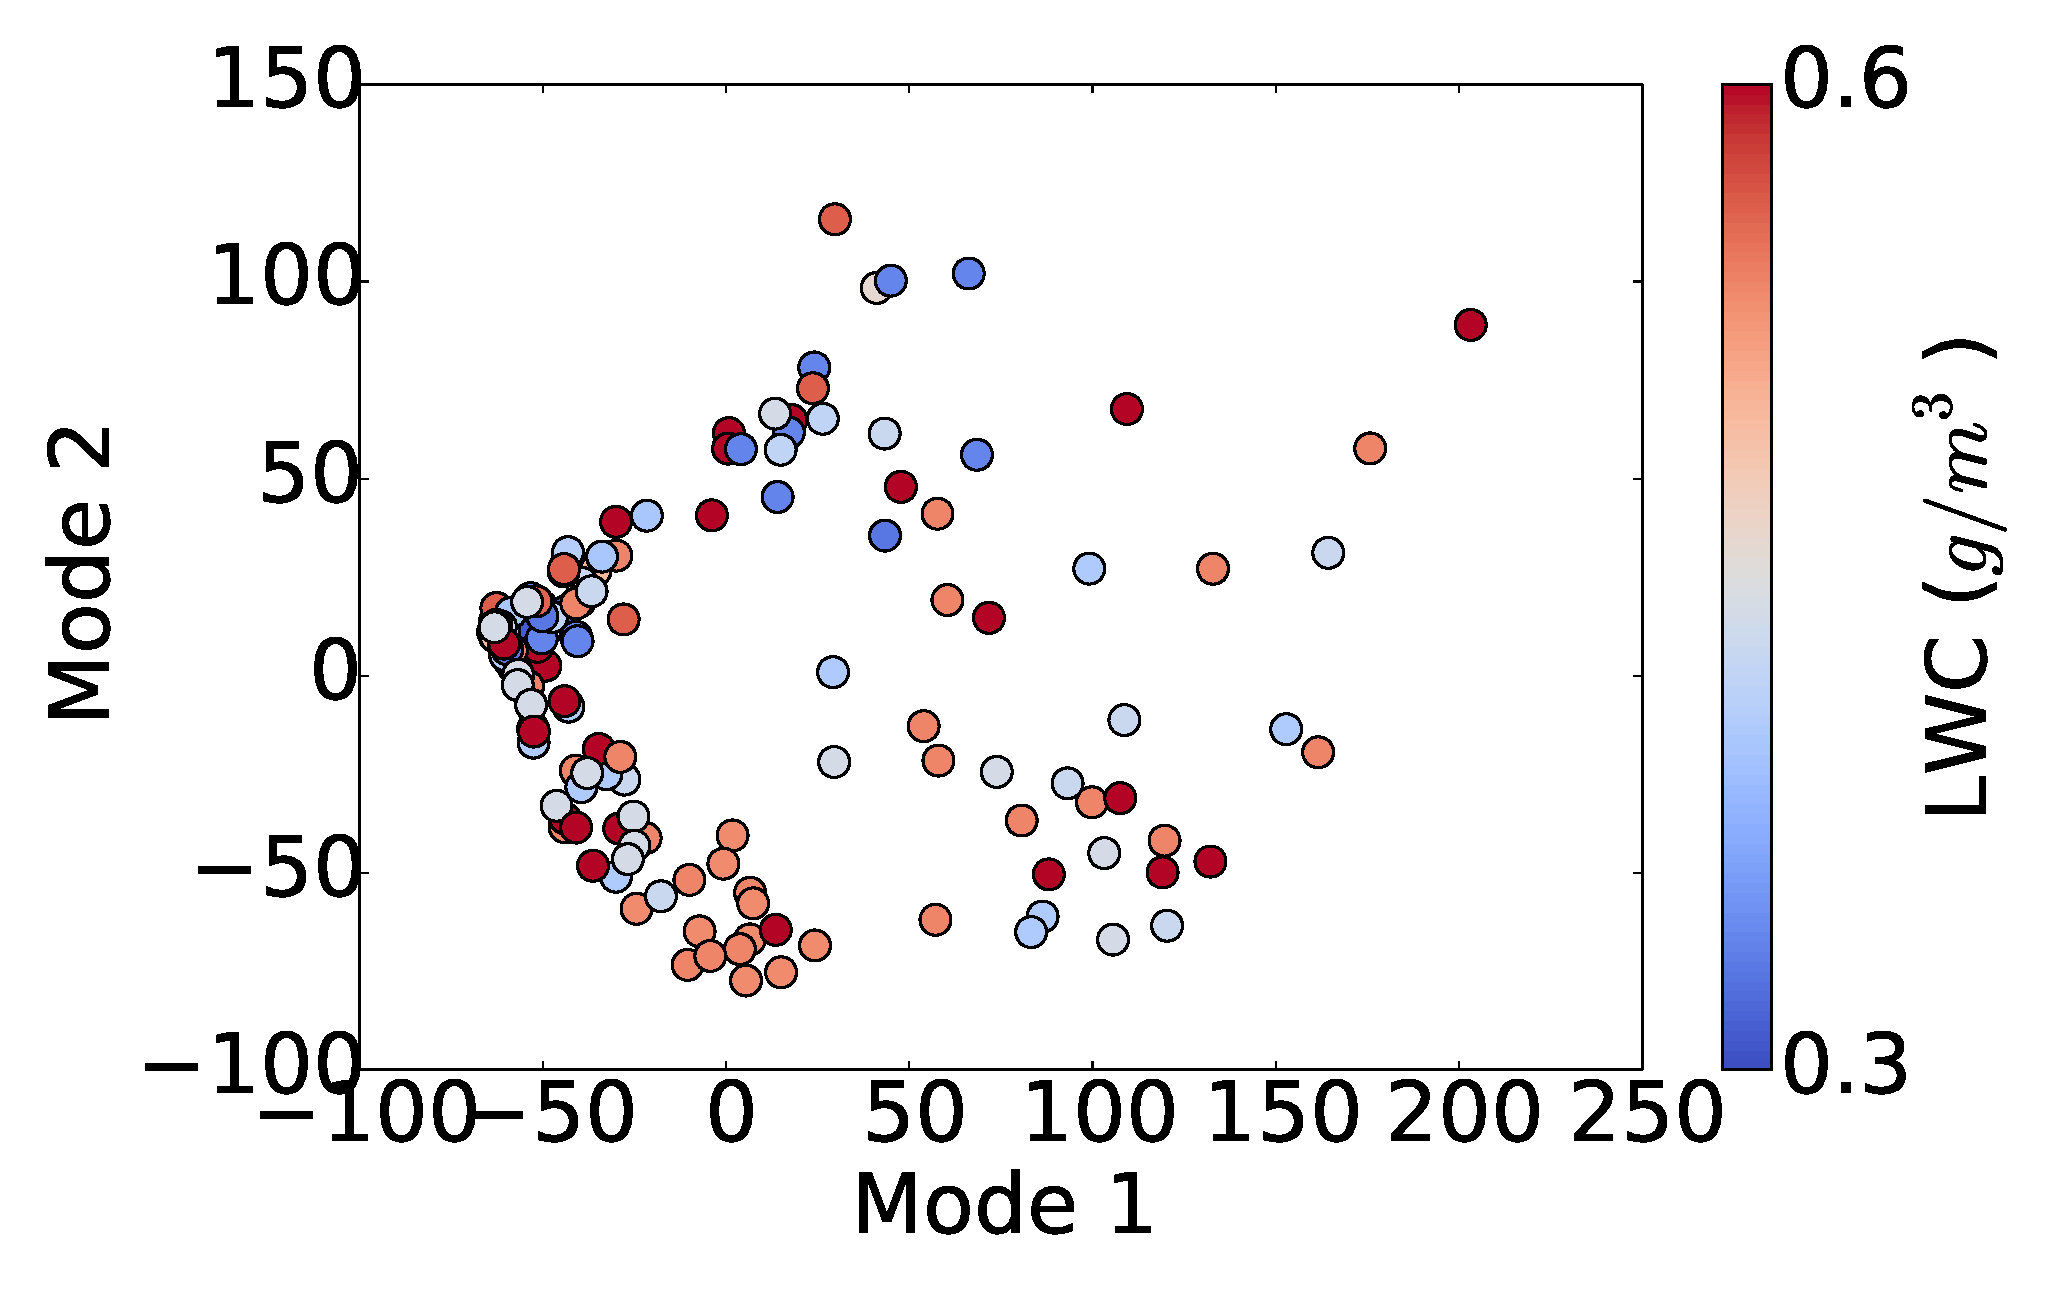
\includegraphics[width=0.35\textwidth]{10ParamMode1Mode2LWC}}
      \vspace*{-0.35cm}\subfigure{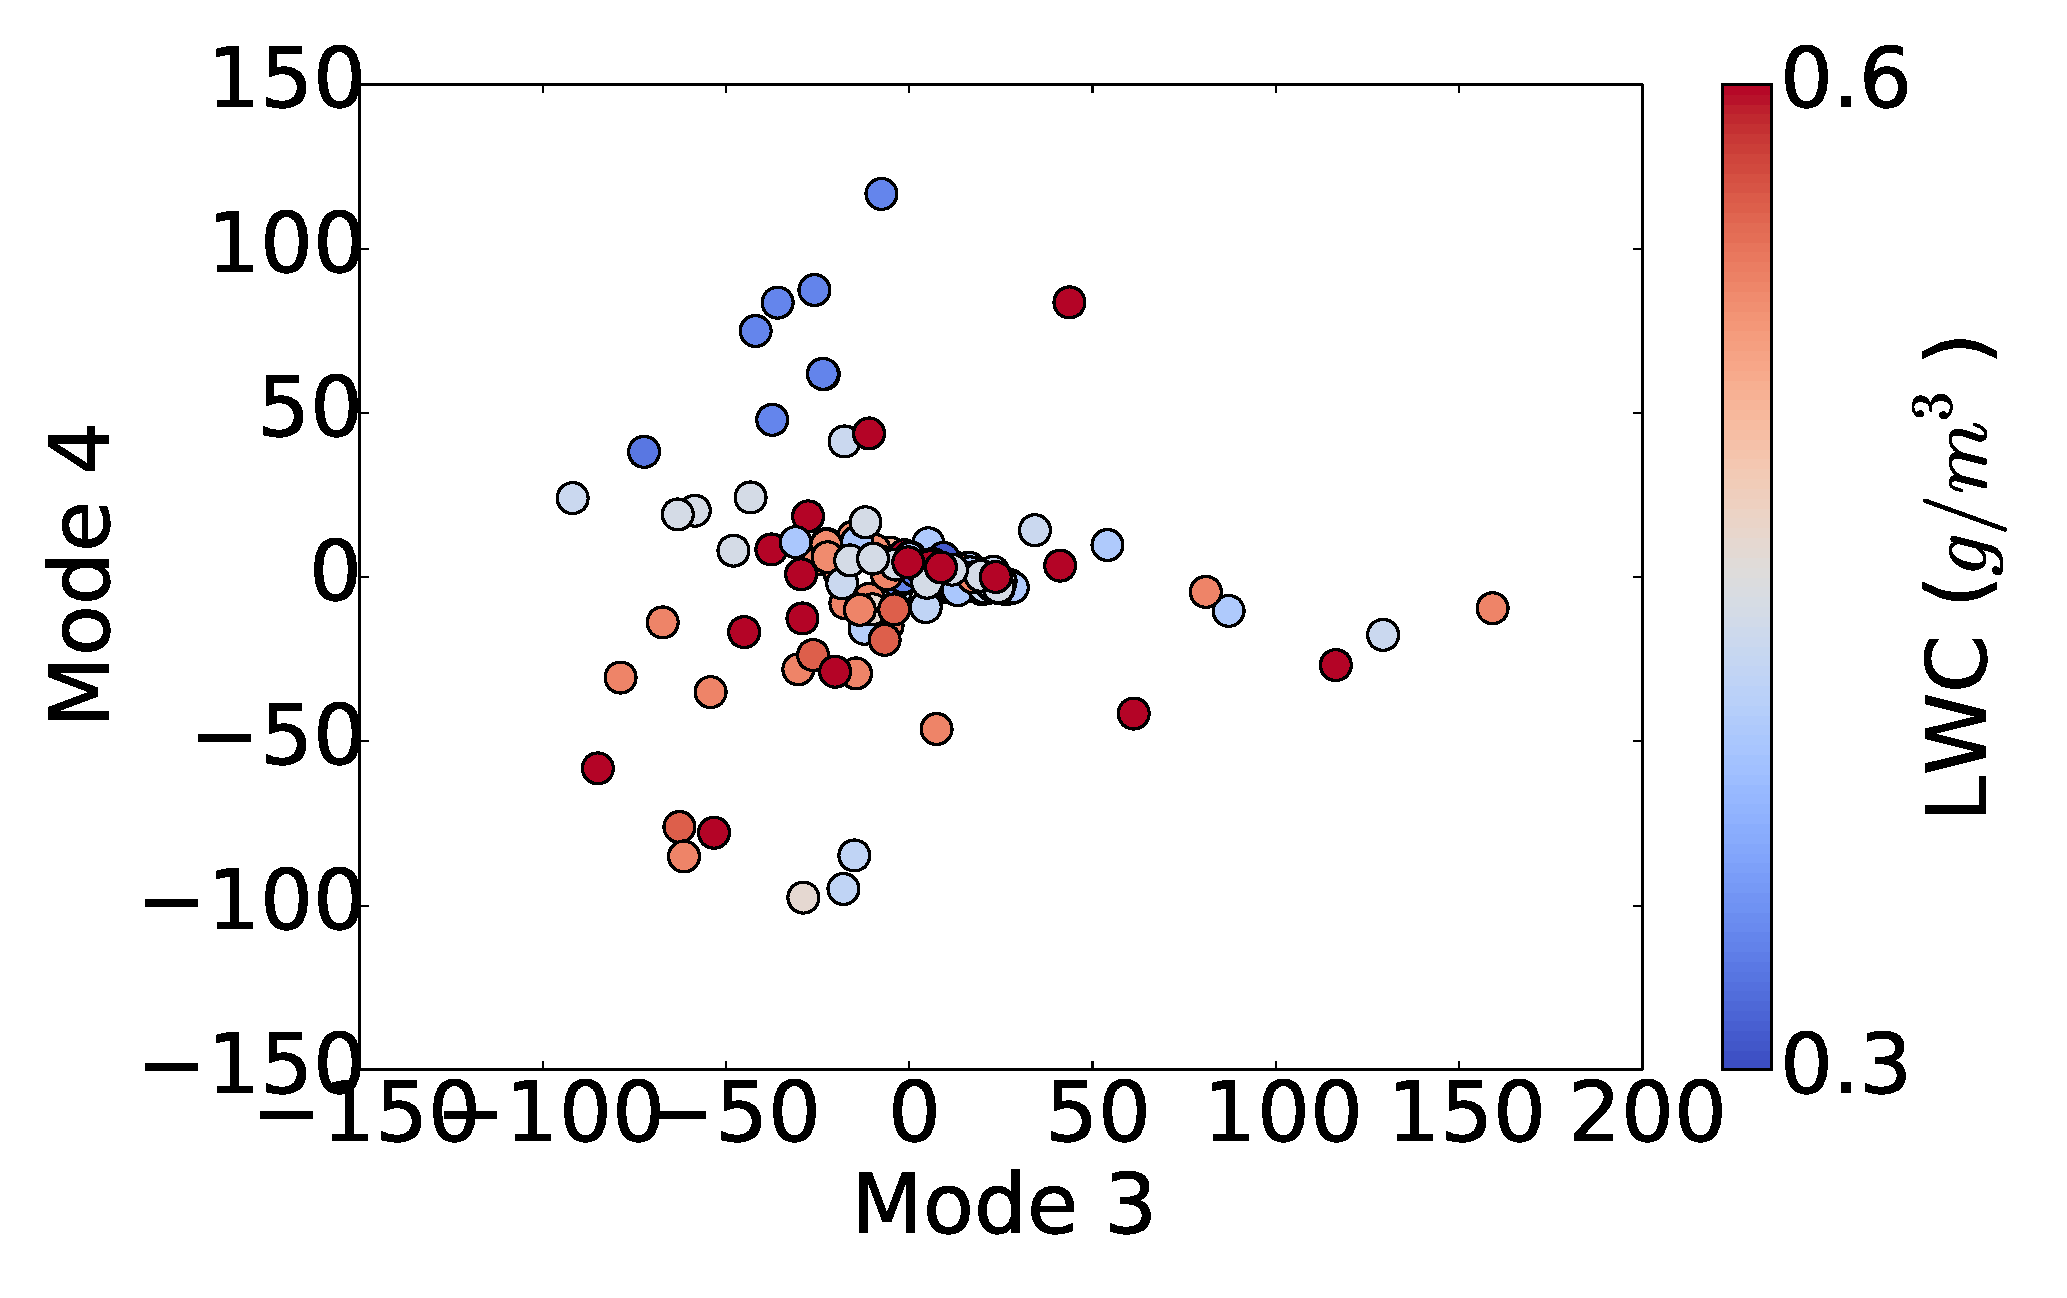
\includegraphics[width=0.35\textwidth]{10ParamMode3Mode4LWC}}
      \vspace*{0cm}\caption{POD coefficients, colored with parameters.}
\end{figure}

\begin{itemize}
\item Statistically relate time, temperature and LWC to POD modes
\item Input conditions, output POD coefficients that respect the data
\end{itemize}
\end{frame}
\begin{frame}
\frametitle{Data-Driven Icing Model}
\label{sec-3-8}

\fontsize{7}\selectfont
% Define the layers to draw the diagram
\pgfdeclarelayer{background}
\pgfdeclarelayer{foreground}
\pgfsetlayers{background,main,foreground}

\begin{figure}[!ht]
  % Define block styles used later
  \tikzstyle{sensor}=[draw, fill=blue!20, text width=5em, 
    text centered, minimum height=2.5em]
  \tikzstyle{ann} = [above, text width=10em, text centered]
  \tikzstyle{wa} = [sensor, text width=8em, fill=blue!20, 
    minimum height=3em, rounded corners]
  % Define distances for bordering
  %\def\blockdist{2.3}
  %\def\edgedist{2.5}
  \vspace*{-1cm}
  \begin{tikzpicture}

    \begin{pgfonlayer}{background}
      \path (1.5,1) node (b) {};
      \path (7.5,-1) node (c) {};
      \path[fill=orange!40,rounded corners, draw=black!50, dashed] (b) rectangle (c);
    \end{pgfonlayer}

    \node (Input) [wa] {{\bf Input}\vspace*{4\em}\\-- Time\\-- Temperature\\-- LWC};
    \path (Input)+(3,0) node (Database) [wa] {{\bf Database}\vspace*{4\em}\\-- Ice shapes\\-- Conditions};
    \path (Database)+(3,0) node (Statistics) [wa] {{\bf Statistics}\vspace*{4\em}\\-- Filtered coeffs\\-- Random samples};
    \path (Statistics)+(3,0) node (Reconstruction) [wa] {{\bf Shape}\vspace*{4\em}\\$\bv{X} = \sum_i^{M} c_i \phi_i$};

    \path [draw, ->, thick] (Input.east) |- node [above] {} (Database.west);
    \path [draw, ->, thick] (Database.east) -- node [below] {} (Statistics.west);
    \path [draw, ->, thick] (Statistics.east) -- node [below] {} (Reconstruction.west);

  \end{tikzpicture}
  \caption{Flowchart of data-driven model.}
\end{figure}
\fontsize{9}\selectfont
\begin{itemize}
\item Input physical condition ranges
\item Filter database for shapes that match conditions
\item Create POD coefficient distributions for downselected data
\item Generate random samples from these distributions
\item Reconstruct ice shape using data-inferred POD coefficients
\end{itemize}
\end{frame}
\begin{frame}
\frametitle{Random Shapes}
\label{sec-3-9}

\begin{figure}
      \vspace*{-0.4cm}\subfigure{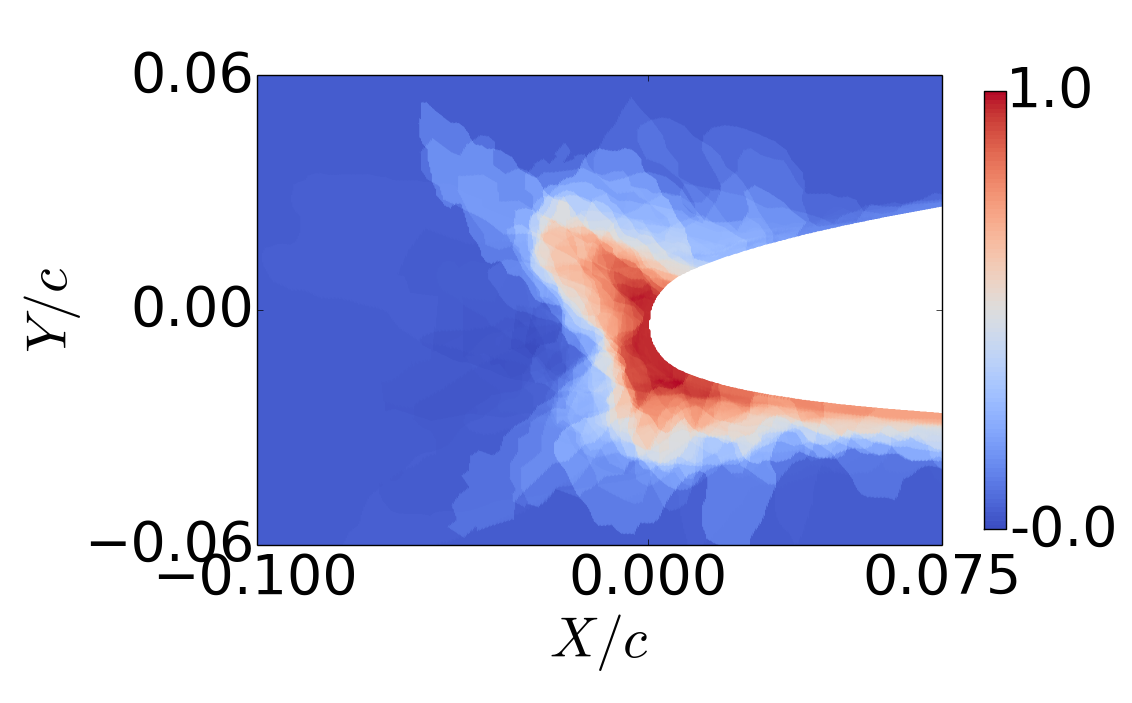
\includegraphics[width=0.4\textwidth]{10ParamHornFromPhysics}}
      \vspace*{-0.4cm}\subfigure{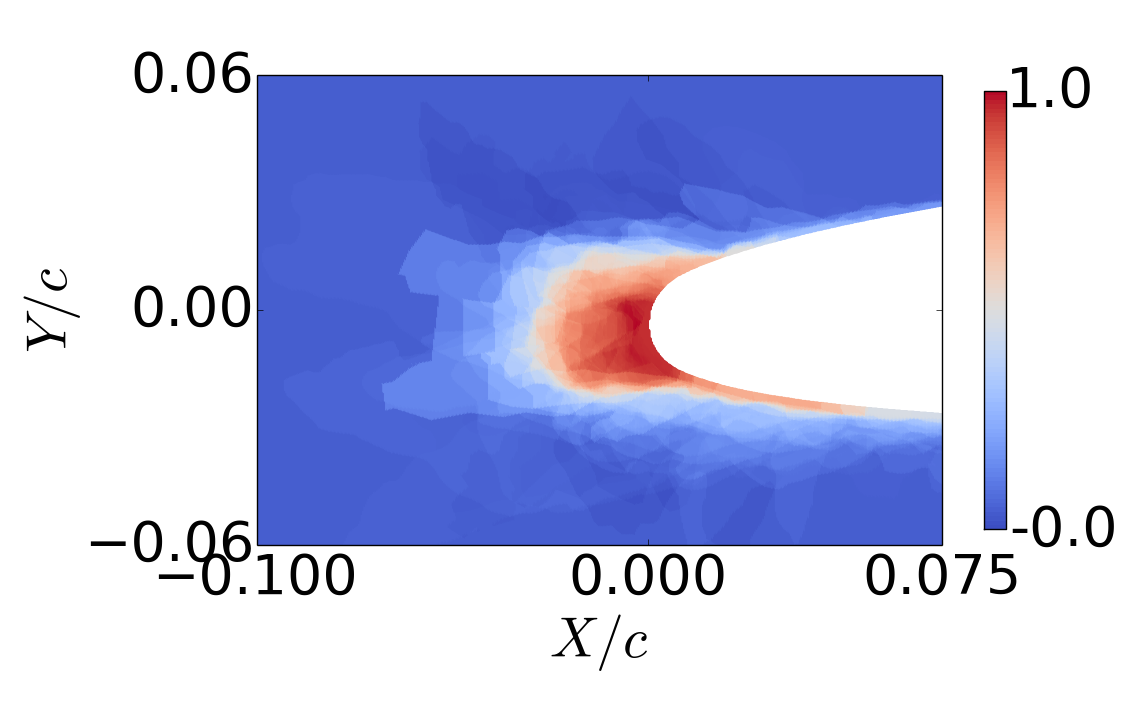
\includegraphics[width=0.4\textwidth]{10ParamRimeFromPhysics}} \\
      \vspace*{-0.4cm}\subfigure[Time > 10 min; temperature > -10 C; LWC > 0.45 $g/m^3$]{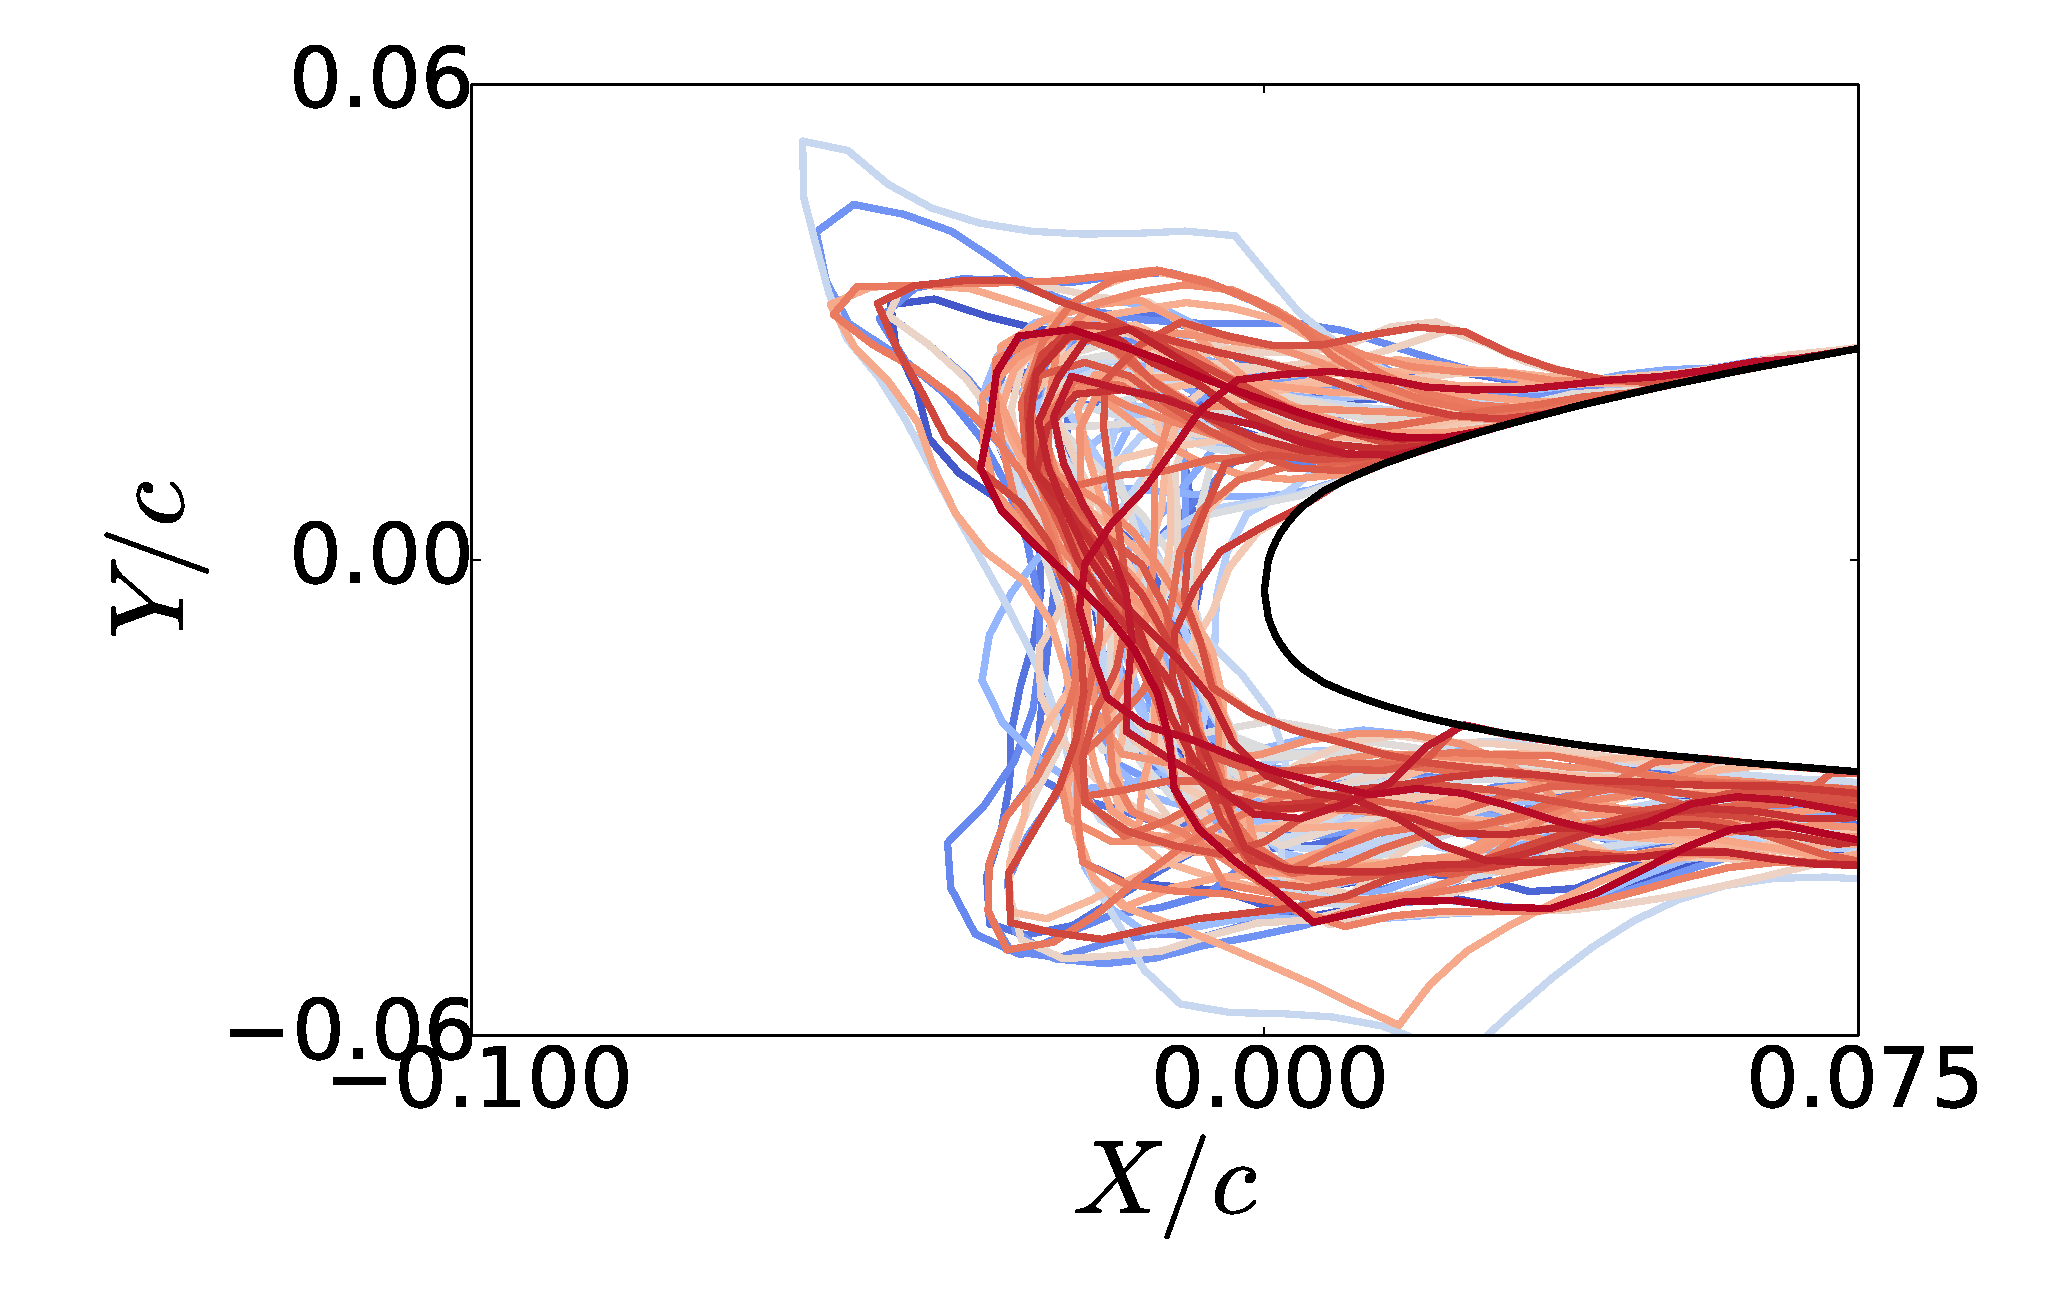
\includegraphics[width=0.4\textwidth]{10ParamRandomHorns}}
      \vspace*{-0.4cm}\subfigure[Time > 10 min; temperature < -10 C; LWC < 0.45 $g/m^3$]{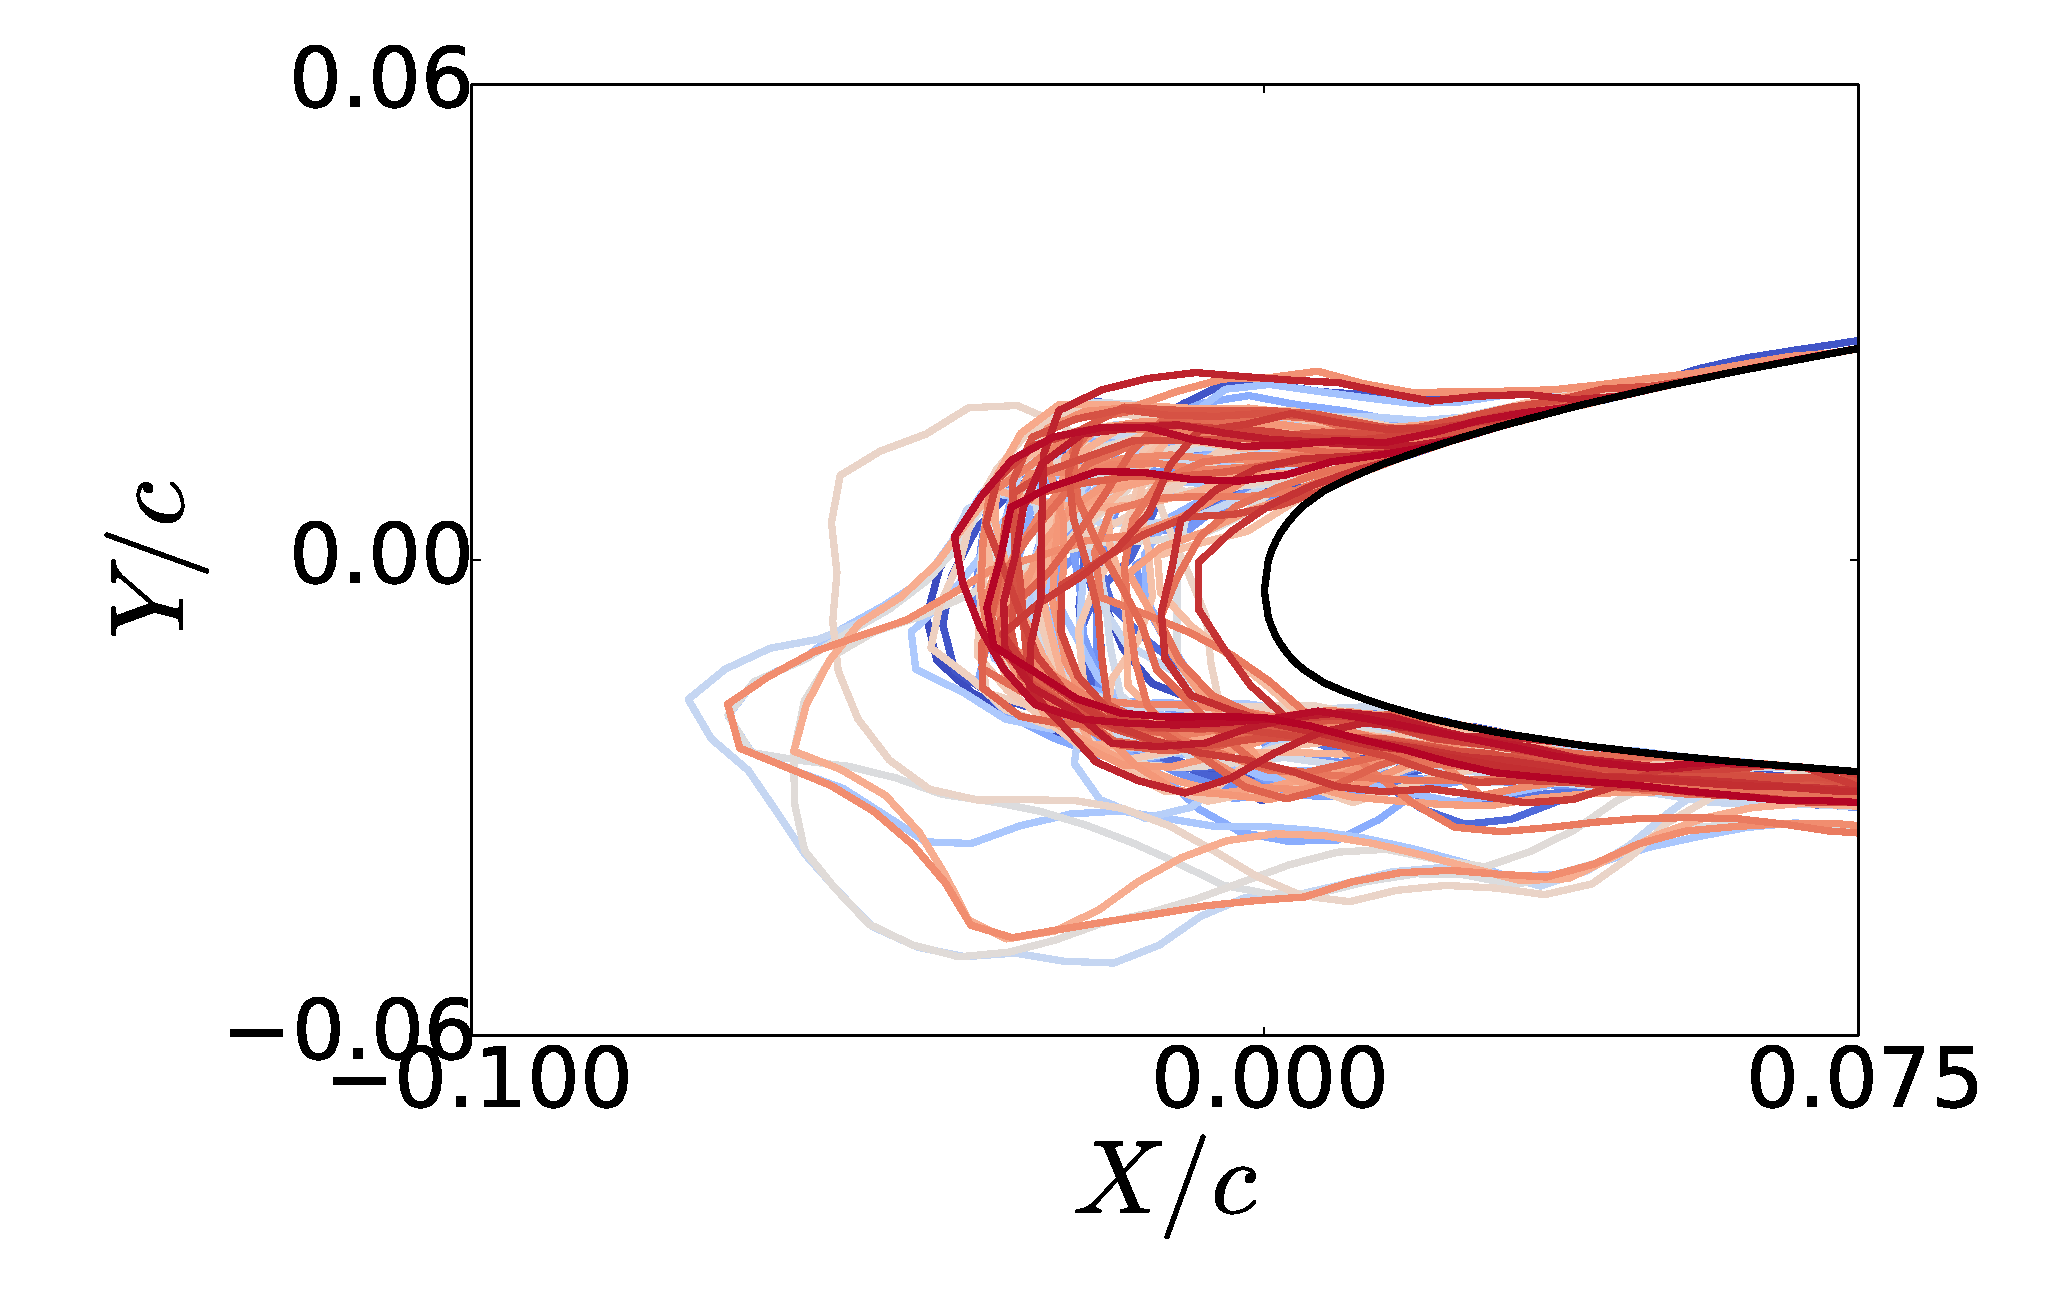
\includegraphics[width=0.4\textwidth]{10ParamRandomRime}}
      \vspace*{0cm}\caption{Random data-driven ice shapes.}
\end{figure}

\begin{itemize}
\item These shapes were generated at random, no physics
\end{itemize}
\end{frame}
\begin{frame}
\frametitle{Uncertainty Quantification}
\label{sec-3-10}

\vspace*{-0.0cm}\begin{figure}
      \includegraphics[width=0.5\textwidth]{GlobalDataSet}
      \caption{Wind tunnel experimental ice shapes}
\end{figure}
\textbf{Goal:} Quantify performance variation with POD modes

\textbf{Approach:}
\begin{itemize}
\item Generate random samples in POD space with Latin Hypercube Sampling (LHS)
\item Test corresponding shapes with flow solver
\item Quantify lift/drag statistics
\end{itemize}
\end{frame}
\begin{frame}
\frametitle{Latin Hypercube Samples}
\label{sec-3-11}

\vspace*{-0.0cm}\begin{figure}
      \vspace*{-1.5cm}\subfigure{\includegraphics[width=0.6\textwidth]{LHS_Shapes}} \\
      \vspace*{-0.5cm}\subfigure{\includegraphics[width=0.35\textwidth]{LHS_Statistics}}
      \vspace*{-0.5cm}\subfigure{\includegraphics[width=0.35\textwidth]{LHS_StatisticsCD}}
      \caption{Latin Hypercube samples.}
\end{figure}
\begin{itemize}
\item 1,921 LHS samples from 10-D modal space
\item LHS statistics reflect database statistics
\end{itemize}
\end{frame}
\begin{frame}
\frametitle{Latin Hypercube Samples}
\label{sec-3-12}

\vspace*{-0.0cm}\begin{figure}
      \subfigure{\includegraphics[width=0.45\textwidth]{LHS_SpatialAvg}}
      \subfigure{\includegraphics[width=0.45\textwidth]{LHS_SpatialVar}}
      \caption{Spatial average and variance.}
\end{figure}
\begin{itemize}
\item Spatial average: lower surface rime accretions are relatively benign
\item Spatial variance: performance sensitive to upper surface horns
\end{itemize}
\end{frame}
\begin{frame}
\frametitle{Dataset}
\label{sec-3-13}

\vspace*{-0.0cm}\begin{figure}
      \includegraphics[width=0.5\textwidth]{GlobalDataSet}
      \caption{Wind tunnel experimental ice shapes}
\end{figure}
\begin{itemize}
\item Dataset consists of 145 experimental ice shapes
\item Obtained in icing wind tunnel at NASA Glenn\footnotemark[1]
\item Representative of a wide variety of icing conditions (temperature,
  LWC, accretion time, etc.)
\end{itemize}
\end{frame}
\begin{frame}
\frametitle{Dataset}
\label{sec-3-14}

\vspace*{-0.0cm}\begin{figure}
      \includegraphics[width=0.5\textwidth]{GlobalDataSet}
      \caption{Wind tunnel experimental ice shapes}
\end{figure}
\textbf{Goals:}
\begin{itemize}
\item Make the ice shapes studied in UQ better reflect observed data
\item Build low-dimensional models to describe complex data
\item Develop empirical ice classification scheme
\end{itemize}
\textbf{Approach:}
\begin{itemize}
\item Cluster ice shapes using spectral graph partitioning
\item Build low-dimensional model using POD
\item Perform parametric UQ on resulting parameter space
\end{itemize}
\end{frame}
\begin{frame}
\frametitle{Distance/Similarity Metric}
\label{sec-3-15}

\vspace*{-0.0cm}\begin{figure}
      \subfigure[XOR Illustration]{\includegraphics[width=0.4\textwidth]{XORexample.png}}
      \subfigure[Dataset Distances]{\includegraphics[width=0.4\textwidth]{XORdistances}}
      \caption{XOR distance metric}
\end{figure}
\begin{itemize}
\item Overlay dataset with a 2D Cartesian grid
\item Assign value of 1 to gridpoint if it is on the ice, 0 otherwise
\item Pick $\sigma$ based on observed peaks in data distances
\item Truncate $w_{ij}$ after $d_{ij} > 3\sigma$
\end{itemize}
\begin{equation*}
w_{ij} = \text{exp} \left(-\frac{1}{2} \frac{d_{ij}^2}{\sigma^2} \right) \;\;\;\;\;\; w_{ij} = \sum_k^{N_G} \left [ \text{XOR}(x_i,x_j) \right ]_k
\end{equation}
 
\end{frame}
\begin{frame}
\frametitle{Spectral Graph Partitioning}
\label{sec-3-16}

\textbf{Goal:} cluster shapes based upon similarity metric \\
\textbf{Methodology:} view database as an undirected graph
$\mathcal{G}(\mathcal{V},\mathcal{E})$
\begin{itemize}
\item Vertices $\mathcal{V}$ are ice shapes
\item Edges $\mathcal{E}$ are similarities between ice shapes
\item Find ``best'' partition of $\mathcal{G}(\mathcal{V},\mathcal{E})$ into subsets A and B
\end{itemize}
\vspace*{-1.25cm}
\begin{figure}
   \includegraphics[width=0.5\textwidth]{GraphPartition.png}
   \vspace{-2.25cm}
   \caption{Graph partition illustration} 
\end{figure}
\end{frame}
\begin{frame}
\frametitle{Spectral Graph Partitioning}
\label{sec-3-17}

\textbf{Approach:}\footnote{Shi \& Malik. \emph{Normalized Cuts and Image Segmentation}, 2000.
 }
\begin{itemize}
\item Calculate graph Laplacian using similarity metric
\begin{itemize}
\item Similarity matrix: $W = w(i,j)$
\item Degree matrix: $D = \text{diag}(d_k) \;\;\; , \;\;\; d_k = \sum_{j=1}^N w(v_k,v_j) \;\;\; , \;\;\; k=1 \cdots N$
\item Laplacian matrix: $L = D - W$
\end{itemize}
\item Eigenvectors with zero eigenvalue identify disconnected subsets
\begin{itemize}
\item E.g., $L \bv{1} = \bv{0}$ <---> entire graph is disconnected
\end{itemize}
\item First nonzero eigenvector (Fiedler vector) identifies optimal
    partition of connected vertices within subsets
\begin{itemize}
\item Approximates solution of \emph{average cut} formulation: \\ 
$P(A,B) = \text{min}_{A \in \mathcal{V}} \left \lbrace \frac{\text{cut}(A,B)}{| A |} + \frac{\text{cut}(A,B)}{| B |} \right \rbrace$ \\
      $|A| = \text{Number of vertices in }A$ \\
      $\text{cut}(A,B) = \sum_{u \in A,v \in B} w(u,v)$
\item Eigenvectors close to zero similarly identify good partitions
\end{itemize}
\end{itemize}
\end{frame}
\begin{frame}
\frametitle{Spectral Graph Partitioning}
\label{sec-3-18}

\begin{figure}
    \includegraphics[width=0.5\textwidth]{ExampleGraph.png}
    \caption{Toy example}
\end{figure}
\begin{equation*}
L = \begin{bmatrix}
1  & -0.9 & -0.1 & 0 & 0 & 0 & 0 \\
-0.9 & 1  & -0.1 & 0 & 0 & 0 & 0 \\
-0.1 & -0.1 & 0.2  & 0 & 0 & 0 & 0 \\
0    & 0    & 0    & 1 & -0.5 & -0.5 & 0 \\
0    & 0    & 0    & -0.5 & 1 & 0 & -0.5 \\
0    & 0    & 0    & -0.5 & 0 & 1 & -0.5 \\
0    & 0    & 0    & 0 & -0.5 & -0.5 & 1 \\ 
\end{bmatrix}
\end{equation}
\end{frame}
\begin{frame}
\frametitle{Spectral Graph Partitioning}
\label{sec-3-19}

\vspace*{-0.0cm}\begin{figure}
      \subfigure[$\lambda_1 = 0$]{\includegraphics[width=0.15\textwidth]{ExampleGraphEvec1.png}}
      \subfigure[$\lambda_2 = 0$]{\includegraphics[width=0.15\textwidth]{ExampleGraphEvec2.png}}
      \caption{Disconnected subsets}
\end{figure}
\vspace*{-0.0cm}\begin{figure}
      \subfigure[$\lambda_3$]{\includegraphics[width=0.15\textwidth]{ExampleGraphEvec3.png}}
      \subfigure[$\lambda_4$]{\includegraphics[width=0.15\textwidth]{ExampleGraphEvec4.png}}
      \subfigure[$\lambda_5$]{\includegraphics[width=0.15\textwidth]{ExampleGraphEvec5.png}}
      \caption{Clustering within subsets}
\end{figure}
\begin{itemize}
\item Two zero eigenvalues, corresponding to two clusters
\item Eigenvalues close to zero give good partitions within clusters
\end{itemize}
\end{frame}
\begin{frame}
\frametitle{Graph Laplacian}
\label{sec-3-20}

\vspace*{-0.0cm}\begin{figure}
      \subfigure[Similarity Matrix]{\includegraphics[width=0.4\textwidth]{DistanceMatrixUnordered.png}}
      \subfigure[Eigenvalue Magnitudes]{\includegraphics[width=0.4\textwidth]{LaplacianEvals}}
      \caption{Laplacian visualization and eigenvalues}
\end{figure}
\begin{itemize}
\item Many zero eigenvalues because many of the dataset elements are
  completely unconnected from each other
\end{itemize}
\end{frame}
\begin{frame}
\frametitle{Clusters}
\label{sec-3-21}

\vspace*{-0.0cm}\begin{figure}
      \subfigure[Similarity Matrix]{\includegraphics[width=0.45\textwidth]{DistanceMatrixOrdered.png}}
      \subfigure[Ice shapes]{\includegraphics[width=0.45\textwidth]{LaplacianUnconnectedCluster}}
      \caption{$\lambda = 0$}
\end{figure}
\begin{itemize}
\item Unconnected cluster represents smaller and less ``extreme'' shapes
\end{itemize}
\end{frame}
\begin{frame}
\frametitle{Clusters}
\label{sec-3-22}

\vspace*{-0.0cm}\begin{figure}
      \subfigure[Similarity Matrix]{\includegraphics[width=0.45\textwidth]{DistanceMatrixOrdered.png}}
      \subfigure[Ice shapes]{\includegraphics[width=0.45\textwidth]{FiedlerVectorGrouping}}
      \caption{Fiedler vector}
\end{figure}
\begin{itemize}
\item Fiedler vector partitions off single most dissimilar member
\end{itemize}
\end{frame}
\begin{frame}
\frametitle{Clusters}
\label{sec-3-23}

\vspace*{-0.0cm}\begin{figure}
      \subfigure[Similarity Matrix]{\includegraphics[width=0.45\textwidth]{DistanceMatrixOrdered2.png}}
      \subfigure[Ice shapes]{\includegraphics[width=0.45\textwidth]{Fiedler2VectorGrouping}}
      \caption{Next smallest eigenvector}
\end{figure}
\begin{itemize}
\item Next smallest eigenvector separates horn and rime accretion
\end{itemize}
\end{frame}
\begin{frame}
\frametitle{POD Coordinates}
\label{sec-3-24}

\vspace*{-0.0cm}\begin{figure}
      \subfigure[POD coordinates]{\includegraphics[width=0.5\textwidth]{ClusterPODcoords}}
      \subfigure[Ice shapes]{\includegraphics[width=0.5\textwidth]{LaplacianUnconnectedCluster}}
      \caption{$\lambda = 0$}
\end{figure}
\end{frame}
\begin{frame}
\frametitle{POD Coordinates}
\label{sec-3-25}

\vspace*{-0.0cm}\begin{figure}
      \subfigure[POD coordinates]{\includegraphics[width=0.5\textwidth]{FiedlerVectorPODcoords}}
      \subfigure[Ice shapes]{\includegraphics[width=0.5\textwidth]{FiedlerVectorGrouping}}
      \caption{Fiedler vector}
\end{figure}
\end{frame}
\begin{frame}
\frametitle{POD Coordinates}
\label{sec-3-26}

\vspace*{-0.0cm}\begin{figure}
      \subfigure[POD coordinates]{\includegraphics[width=0.5\textwidth]{Fiedler2VectorPODcoords}}
      \subfigure[Ice shapes]{\includegraphics[width=0.5\textwidth]{Fiedler2VectorGrouping}}
      \caption{Next smallest eigenvector}
\end{figure}
\end{frame}
\begin{frame}
\frametitle{Cluster Modeling}
\label{sec-3-27}

\vspace*{-0.75cm}\begin{figure}
      \subfigure[$S$-Coordinates]{\includegraphics[width=0.35\textwidth]{ScoordsCluster1}}
      \subfigure[POD Eigenvalues]{\includegraphics[width=0.35\textwidth]{PODevalsCluster1}}
      \subfigure[Mean]{\includegraphics[width=0.35\textwidth]{MeanCluster1}}
      \subfigure[POD Modes]{\includegraphics[width=0.35\textwidth]{PODmodes1to5Cluster1}}
      \caption{POD of ice shape cluster}
\end{figure}
\textbf{Goal:} build a low-dimensional model of ice shape cluster for UQ
\end{frame}
\begin{frame}
\frametitle{Cluster Modeling}
\label{sec-3-28}

\vspace*{-0.0cm}\begin{figure}
      \subfigure[Mode 1]{\includegraphics[width=0.3\textwidth]{POD1Shapes3Sig}}
      \subfigure[Mode 2]{\includegraphics[width=0.3\textwidth]{POD2Shapes3Sig}}
      \subfigure[Mode 3]{\includegraphics[width=0.3\textwidth]{POD3Shapes3Sig}}
      \subfigure[Mode 4]{\includegraphics[width=0.3\textwidth]{POD4Shapes3Sig}}
      \subfigure[Mode 5]{\includegraphics[width=0.3\textwidth]{POD5Shapes3Sig}}
      \caption{Ice model modes}
\end{figure}
Variations shown about dataset mean ($\pm 3 \sigma$)
\end{frame}
\begin{frame}
\frametitle{Parameter Space}
\label{sec-3-29}

\vspace*{-0.0cm}\begin{figure}
      \subfigure[Mode 1]{\includegraphics[width=0.3\textwidth]{Cluster1Coeff1PDF}}
      \subfigure[Mode 2]{\includegraphics[width=0.3\textwidth]{Cluster1Coeff2PDF}}
      \subfigure[Mode 3]{\includegraphics[width=0.3\textwidth]{Cluster1Coeff3PDF}}
      \subfigure[Mode 4]{\includegraphics[width=0.3\textwidth]{Cluster1Coeff4PDF}}
      \subfigure[Mode 5]{\includegraphics[width=0.3\textwidth]{Cluster1Coeff5PDF}}
      \caption{Mode statistics ({\color{blue} data} and {\color{red} fit})}
\end{figure}
\begin{itemize}
\item Fit a normal distribution to dataset statistics
\item 5-dimensional UQ study with all Gaussian variables
\end{itemize}
\end{frame}
\begin{frame}
\frametitle{Output Statistics}
\label{sec-3-30}

\vspace*{-0.0cm}\begin{figure}
      \subfigure[PDF($C_L$)]{\includegraphics[width=0.4\textwidth]{PDFCLTOL1em4}}
      \subfigure[PDF($C_D$)]{\includegraphics[width=0.4\textwidth]{PDFCDTOL1em4}}
      \caption{Output PDFs for lift and drag}
\end{figure}
\textbf{Setup}
\begin{itemize}
\item Business jet clean airfoil\footnotemark[1], $\alpha = 3^{\circ}$, $Re = 7.5\times10^6$
\item FLO103 code (2D steady-state RANS solver)
\item Adaptive sparse grid collocation for PCE, implemented with DAKOTA
\end{itemize}
\textbf{Results}
\begin{itemize}
\item PC surrogate converged using 487 solver evaluations
\end{itemize}
\end{frame}
\begin{frame}
\frametitle{Global Extrema}
\label{sec-3-31}

\vspace*{-0.0cm}\begin{figure}
      \subfigure[Highest decile of $C_L$]{\includegraphics[width=0.3\textwidth]{BoxplotHighCL}}
      \subfigure[Lowest decile of $C_L$]{\includegraphics[width=0.3\textwidth]{BoxplotLowCL}}
      \subfigure[Means of top and bottom deciles]{\includegraphics[width=0.3\textwidth]{GoodBadAirfoils}}
      \caption{Global extrema visualized}
\end{figure}
\begin{itemize}
\item \textbf{Good:} low accretion, smooth, conforms to airfoil surface
\item \textbf{Bad:} high accretion, horns, protrude out as flow obstacles
\end{itemize}
\end{frame}
\section{Computational UQ}
\label{sec-4}
\begin{frame}
\frametitle{Motivation}
\label{sec-4-1}

\textbf{Investigate uncertainty in the physical process of icing}
\begin{itemize}
\item What is the statistical effect of uncertainty in physical parameters?
\begin{itemize}
\item Free-stream temperature
\item Liquid water content (LWC)
\item Accretion time
\item Droplet diameter distribution (MVD)
\item Surface roughness
\end{itemize}
\item Want to quantify how perturbations of the physics affects aerodynamics
\end{itemize}
\end{frame}
\begin{frame}
\frametitle{Airfoil Icing Code Flowchart}
\label{sec-4-2}

\fontsize{7}\selectfont
% Define the layers to draw the diagram
\pgfdeclarelayer{background}
\pgfdeclarelayer{foreground}
\pgfsetlayers{background,main,foreground}

\begin{figure}[!ht]
  % Define block styles used later
  \tikzstyle{sensor}=[draw, fill=blue!20, text width=5em, 
    text centered, minimum height=2.5em]
  \tikzstyle{ann} = [above, text width=10em, text centered]
  \tikzstyle{wa} = [sensor, text width=10em, fill=blue!20, 
    minimum height=3em, rounded corners]
  % Define distances for bordering
  %\def\blockdist{2.3}
  %\def\edgedist{2.5}
  \vspace*{-1cm}
  \begin{tikzpicture}

    \begin{pgfonlayer}{background}
      \path (2,4) node (a) {};
      \path (6,-3.5) node (b) {};
      \path[fill=orange!40,rounded corners, draw=black!50, dashed] (a) rectangle (b);
    \end{pgfonlayer}

    \node (CleanAirfoil) [wa] {\includegraphics[width=0.6\textwidth]{ExampleCleanAirfoil}\\\bf{Clean Airfoil}};
    \path (CleanAirfoil)+(4,2.5) node (FlowSolver) [wa] {\includegraphics[width=0.6\textwidth]{ExampleSoln}\\\bf{Mesh/Flow Solver}};
    \path (FlowSolver)+(0,-2) node (Droplet) [wa] {\includegraphics[width=0.6\textwidth]{DropletAdvectionR10}\\\bf{Droplet Simulation}};
    \path (Droplet)+(0,-1.5) node (ThermoModule) [wa] {$\frac{\partial \bm{F}}{\partial t} + \nabla \cdot \bm{F} = \dot{\bm{S}}$ \\\bf{Thermodynamics}};
    \path (ThermoModule)+(0,-1.5) node (IcedAirfoil) [wa] {\includegraphics[width=0.6\textwidth]{ExampleIceGrowth}\\\bf{Iced Geometry}};
    \path (CleanAirfoil)+(8,0) node (FinalAirfoil) [wa] {\includegraphics[width=0.6\textwidth]{ExampleIceGrowthFinal}\\\bf{Final Geometry}};

    \path [draw, ->, thick] (CleanAirfoil.north) |- node [above] {} (FlowSolver.west);
    \path [draw, ->, thick] (FlowSolver.south) -- node [below] {} (Droplet.north);
    \path [draw, ->, thick] (Droplet.south) -- node [below] {} (ThermoModule.north);
    \path [draw, ->, thick] (ThermoModule.south) -- node [below] {} (IcedAirfoil.north);
    \path [draw, ->, thick] (IcedAirfoil.east) -| node [above] {} (FinalAirfoil.south);
    \path [draw, ->, thick] (IcedAirfoil.east) -- ++(0.25,0cm) |- node [above]
          {} (FlowSolver.east);

  \end{tikzpicture}

\end{figure}
\end{frame}
\begin{frame}
\frametitle{Droplet Advection}
\label{sec-4-3}

\textbf{Advection Equations:} \\
\begin{equation*}
  \begin{align}
    \frac{d \bv{x}}{d t} &= \bv{v} \\
    m \frac{d \bv{v}}{d t} &= \frac{1}{2} \rho_g C_D \pi r^2 ||\bv{v_g} - \bv{v}|| (\bv{v_g} - \bv{v}) + m \bv{g}
  \end{align}
\end{equation}

\begin{columns}[c]
  \column{0.5\textwidth}
    \centering
    \begin{figure}
    \includegraphics[width=0.9\textwidth]{DropletAdvection_NACA0012_R10}
    \caption{R = 10$\mu$m}
    \end{figure}
  \column{0.5\textwidth}
    \centering
    \begin{figure}
    \includegraphics[width=0.9\textwidth]{DropletAdvection_NACA23012_R118} \\
    \caption{R = 118$\mu$m}
    \end{figure}
\end{columns}
\end{frame}
\begin{frame}
\frametitle{Thermodynamics}
\label{sec-4-4}

\textbf{Conservation Equations:} \\
\begin{equation*}
  \begin{align}
    \rho_w \left \lbrace \frac{\partial h_f}{\partial t} + \nabla \cdot (\bv{u_f} h_f) \right \rbrace &= \dot{m}_{imp} - \dot{m}_{evap} - \dot{m}_{ice} \\
    \rho_w \left \lbrace \frac{\partial (h_f c_W T)}{\partial t} + \nabla \cdot (\bv{u_f} h_f c_W T) \right \rbrace &= \left [ c_W T_d + \frac{u_d^2}{2} \right ] \dot{m}_{imp} \\
    & - L_{evap} \dot{m}_{evap} \\
    & +(L_{fus} + c_{ice}T)\dot{m}_{ice} \\
    & + c_H (T_{Rec} - T)
  \end{align}
\end{equation}

\begin{itemize}
\item \textbf{Mass}
\begin{itemize}
\item Enters through impinging droplets
\item Exits via evaporation/sublimation and freezing
\end{itemize}
\item \textbf{Energy}
\begin{itemize}
\item Enters through impinging droplets, freezing of ice
\item Exits via evaporation/sublimation, radiation, convection
\end{itemize}
\item Solution procedure: explicit marching, finite volume discretization
  with upwinded derivatives
\end{itemize}
\end{frame}
\begin{frame}
\frametitle{Thermodynamics Solution Procedure}
\label{sec-4-5}

\begin{columns}[c]
\column{0.4\textwidth}
\hspace*{-0.5cm}
\scalebox{0.8}{
\begin{equation*}
\begin{aligned}
\frac{\partial U}{\partial t} + \frac{\partial F}{\partial s} &= \dot{S} \\
\int_{\mathcal{B}_k} \left( \frac{\partial U}{\partial t} + \frac{\partial F}{\partial s} \right) \;ds &= \int_{\mathcal{B}_k} \dot{S}\; ds \\
\int_{\mathcal{B}_k} \frac{\partial U}{\partial t}\;ds + \left( F_{k+1/2} - F_{k-1/2} \right) &= \int_{\mathcal{B}_k} \dot{S}\; ds \\
\frac{\partial \bar{U}_k}{\partial t} = \mathrlap{\underbrace{ \frac{1}{\Delta s_k} \int_{\mathcal{B}_k} \dot{S}\; ds - \Delta F_k }_{ \delta_u }} \\
\bar{U}_k^{t+\Delta t} &= \bar{U}_k^{t} - \Delta t \delta_u
\end{aligned}
\end{equation}
}
\column{0.6\textwidth}
\centering
\begin{figure}[ht]
  \centering
  \includegraphics[trim=70mm 20mm 270mm 20mm,clip,width=1\textwidth]{FiniteVolume}
  \caption{Finite volume method.}
\end{figure}
\end{columns}
\begin{itemize}
\item Finite volume discretization of equations
\item Roe scheme flux calculation (upwinding)
\end{itemize}
\end{frame}
\begin{frame}
\frametitle{Validations}
\label{sec-4-6}

\vspace*{-0.5cm}
\begin{figure}[ht]
  \centering
  \includegraphics[trim=0.625in 0.75in 0.83in 0.8in,clip,width=0.6\textwidth]{IceShapeValidations.png}
  \caption{Experiment ({\color{red} red}), LEWICE ({\color{green} green}), and CATFISh ({\color{blue} blue}).}
\end{figure}
\end{frame}
\begin{frame}
\frametitle{UQ Study: Temp + LWC}
\label{sec-4-7}

\begin{figure}[ht]
\centering
\subfigure[Quadrature points (colorscale identical to (b)).]{\includegraphics[width=0.3\textwidth]{QuadPts_2ParamCLalpha}}
\subfigure[PCE surrogate.]{\includegraphics[width=0.3\textwidth]{Map_2ParamCLalpha.png}}
\subfigure[PCE surrogate statistics.]{\includegraphics[width=0.3\textwidth]{Statistics_2ParamCLalpha}}
\caption{Quadrature points, PCE surrogate, and statistics for the 2 parameter ($T_{\infty}$ and LWC) study on lift slope.}
\end{figure}
\end{frame}
\begin{frame}
\frametitle{UQ Study: Temp + LWC + Time}
\label{sec-4-8}

\begin{figure}[ht]
\centering
\subfigure[Quadrature points (colorscale identical to (b)).]{\includegraphics[trim=20mm 0mm 35mm 0mm,clip,width=0.3\textwidth]{3Param_TinfLWCDT_QuadPts}}
\subfigure[PCE surrogate (parameter units identical to (a)).]{\includegraphics[width=0.3\textwidth]{3Param_TinfLWCDT_Map.png}}
\subfigure[Ice shapes at quadrature points (colorscale identical to (c)).]{\includegraphics[width=0.3\textwidth]{3Param_TinfLWCDT_Shapes}}
\subfigure[PCE surrogate statistics.]{\includegraphics[width=0.3\textwidth]{3Param_TinfLWCDT_Statistics}}
\subfigure[Statistics of $C_{L_{\alpha}}$ as a function of $\Delta$T.]{\includegraphics[width=0.3\textwidth]{3Param_TinfLWCDT_CondExp}}
\caption{Quadrature points, PCE surrogate, and statistics.}
\end{figure}
\end{frame}
\begin{frame}
\frametitle{UQ Study: Temp + LWC + Roughness}
\label{sec-4-9}

\begin{figure}[ht]
\centering
\subfigure[Quadrature points (colorscale identical to (b)).]{\includegraphics[trim=20mm 0mm 35mm 0mm,clip,width=0.3\textwidth]{3Param_TinfLWCRough_QuadPts}}
\subfigure[PCE surrogate (parameter units identical to (a)).]{\includegraphics[width=0.3\textwidth]{3Param_TinfLWCRough_Map.png}}
\subfigure[Ice shapes at quadrature points (colorscale identical to (c)).]{\includegraphics[width=0.3\textwidth]{3Param_TinfLWCRough_Shapes}}
\subfigure[PCE surrogate statistics.]{\includegraphics[width=0.3\textwidth]{3Param_TinfLWCRough_Statistics}}
\subfigure[Statistics of $C_{L_{\alpha}}$ as a function of $\Delta$T.]{\includegraphics[width=0.3\textwidth]{3Param_TinfLWCRough_CondExp}}
\caption{Quadrature points, PCE surrogate, and statistics.}
\end{figure}
\end{frame}
\begin{frame}
\frametitle{Conclusions}
\label{sec-4-10}

\textbf{Problems:}
\begin{itemize}
\item Wing icing deteriorates icing aerodynamics, danger to safe flight
\item Ice shapes are diverse and complex
\item Not clear what the exact aerodynamic effects of different shapes are
\item Would like systematic way of exploring airfoil icing through data
\end{itemize}
\textbf{Solutions:}
\begin{itemize}
\item Data-driven approach
\begin{itemize}
\item Build empirical model of ice accretion from data
\item Perform parametric UQ to quantify range of performance
\end{itemize}
\item Computational approach
\begin{itemize}
\item Build computational ice accretion code from scratch
\item Perform parametric UQ to quantify effects of physics
\end{itemize}
\end{itemize}







 
\end{frame}

\end{document}
